 % to sort

% figures
% sphere coord needs middlie red line to get slice count consistent
% torus diagram needs colour
% check captions
% make inkscape pdf
% add figures for types of radiation and applications
% clean cuttubs fig

% equations for motion of a particle
% need to have local copy of code if it changes in appendix listings
% polycone stack kept at 3
% conversion typically leads to leads to loss of detail -> pyg4ometry and GUIMesh are free (open-source) alternatives to this (mesh deviation stuff?)

% table of sphere comps
% G4 total unrestricted stopping power mathes with paper
% boolean symbols latex
% check all units
% cheack for TODO

% reference section
% format
% check refs and cites
% ref VTK
% ref table in diff latex doc ?
% portugal paper ref

%to check at end
% check pagegaps
% check no null ref or cites
% put newpage in table of contents

% stopping power equations
% descibe a collimator
% bdsim is compared with experiment
%nuclear waste storage
% read pyg4omety paper in docs 
% with secs on old becomes slower than new 
% types of radiation are in bdsim
%fix med max legend (use New + Median)

% questions 
% is brem and cherenokov within ftfp_bert ?
% cherenkov no s it produces an amazing number of photons (makes tracking slow) and they're very low energy so not often cared about

\documentclass[12pt,a4paper]{article}
\usepackage{graphicx}
\usepackage{hyperref}   
\usepackage{braket}
\usepackage{amsmath}

\usepackage[utf8]{inputenc}
\usepackage[english]{babel}

\usepackage{listings}
\usepackage{color}
\usepackage[margin=0.75in]{geometry}
\usepackage{subfigure}

\definecolor{mygreen}{rgb}{0,0.6,0}
\definecolor{mygray}{rgb}{0.5,0.5,0.5}
\definecolor{mymauve}{rgb}{0.58,0,0.82}
\usepackage{afterpage}

\newcommand{\ts}{\textsuperscript}
\usepackage[super]{nth}
\usepackage{gensymb}
\usepackage{xcolor}
\usepackage{wasysym}
%\usepackage{wasysym} %for astro symbols

 \lstset{ 
  backgroundcolor=\color{white},  % choose the background color; you must add \usepackage{color} or \usepackage{xcolor}; should come as last argument
  basicstyle=\footnotesize,             % the size of the fonts that are used for the code
  breakatwhitespace=false,            % sets if automatic breaks should only happen at whitespace
  breaklines=true,                          % sets automatic line breaking
  captionpos=b,                             % sets the caption-position to bottom
  commentstyle=\color{mygreen},   % comment style
  deletekeywords={...},                   % if you want to delete keywords from the given language
  escapeinside={\%*}{*)},             % if you want to add LaTeX within your code
  extendedchars=true,                    % lets you use non-ASCII characters; for 8-bits encodings only, does not work with UTF-8
  frame=single,	                            % adds a frame around the code
  keepspaces=true,                         % keeps spaces in text, useful for keeping indentation of code (possibly needs columns=flexible)
  keywordstyle=\color{blue},            % keyword style
  language=Octave,                         % the language of the code
  morekeywords={*,...},                  % if you want to add more keywords to the set
  numbers=left,                               % where to put the line-numbers; possible values are (none, left, right)
  numbersep=5pt,                            % how far the line-numbers are from the code
  numberstyle=\tiny\color{mygray},   % the style that is used for the line-numbers
  rulecolor=\color{black},                 % if not set, the frame-color may be changed on line-breaks within not-black text (e.g. comments (green here))
  showspaces=false,                        % show spaces everywhere adding particular underscores; it overrides 'showstringspaces'
  showstringspaces=false,               % underline spaces within strings only
  showtabs=false,                           % show tabs within strings adding particular underscores
  stepnumber=2,                             % the step between two line-numbers. If it's 1, each line will be numbered
  stringstyle=\color{mymauve},        % string literal style
  tabsize=2,	                             % sets default tabsize to 2 spaces
  title=\lstname                               % show the filename of files included with \lstinputlisting; also try caption instead of title
} 

\usepackage{multicol}
\usepackage[font=small,labelfont=bf]{caption} % Makes the font for figure captions smaller and the figure label bold.

\begin{document}
%\pagecolor{black}\afterpage{\nopagecolor}
%\color{white}
\begin{titlepage}
	\centering
	
\includegraphics[width=0.4\textwidth]{Images//Logos//rhul.jpg}\par\vspace{1cm}


	{\scshape\LARGE Royal Holloway University of London \par}
	\vspace{1cm}
	{\scshape\Large PH4100: Major Project\par}
	\vspace{1.5cm}
	{\huge\bfseries Meshing of Primitive Solids\\
	in\\
	Pyg4ometry \& BDSIM\par}
	\vspace{2cm}
	{\Large\itshape Ben Shellswell\par}
	\vfill

\begin{abstract}
\centering

\end{abstract}
The testing and analysis of radiation travelling through geometries of devices, such as a medical magnets, spacecraft or new particle accelerators, is often a very expensive and time consuming process. The open-source software packages Pyg4ometry \& BDSIM are designed to enable scientists and people within many different industries to virtually simulate these tests, with accurate physics concepts. This project looks at improving the 3D simulation of the events and devices, by the remeshing of the basic primitive solids and testing them in BDSIM.

	\vfill
	
	Supervised by\par
	Prof.~S \textsc{Boogert} 

% Bottom of the page
	{\large \today\par}



\begin{figure}[h]
\centering
\begin{minipage}{.6\textwidth}
  
\includegraphics[width=0.4\textwidth]{Images//Logos//BDSIM_Logo.jpg}
\end{minipage}%
\begin{minipage}{.6\textwidth}
  \centering
  
\includegraphics[width=0.5\textwidth]{Images//Logos//JAI_Logo.jpeg}
  \end{minipage}
\end{figure}

\end{titlepage}
\leavevmode\thispagestyle{empty}\newpage
%\color{black}
%\footnotesize
\tableofcontents
\normalsize
\thispagestyle{empty}
\newpage
\onecolumn

%%%%%%%%%%%%%%%%%%%%%%%%%%%%%%%%%%%%%%%%%%%%%%%%%%%%%%%%%%%%%%%%%%%%%%
\small
\setcounter{page}{1}

% ------------------------------------------------------------------------------------------------------------------------------

\section{Introduction}

\subsection{Report Structure}
The following subsections of the introduction will go on to discuss the background (Section \ref{back}), motivations (Section \ref{motiv}) and aims (Section \ref{aim}) of the project. Then the subsequent Sections are structured in the following way; first a discussion of the types of radiation emission (Section \ref{radd}), the software packages that are used and referenced throughout this report are discussed in Section \ref{packs}, the concepts and details of the primitive meshing used in Pyg4ometry (Section \ref{prim}). The interactions of meshed solids and objects in BDSIM (Section \ref{int}) and a conclusion and summary of the results of the report (Section \ref{conc}). Followed by an Appendix \ref{ap1}, which lists a variety of content produced in the project, but is not included in the report its self, in the interest of being incise.

\subsection{Project Background - Applications of Particle Tracking}
\label{back}
On Earth we experience harmless radiation everyday, for example small doses of UV (or UltraViolet) radiation from the Sun. However in many cases radiation is unwanted and/or needs to be controlled, which is where the simulations of radiation transport comes into play. Radiation transport is the physical phenomenon of energy transfer through a medium in the form of electromagnetic radiation. The various types of radiation are discussed in Section \ref{radd}. There is a large number of sectors that the simulation of particle radiation tracking is an invaluable tool.

\subsubsection{High Energy Physics}
\noindent The most obvious field in which radiation transport is important is all things nuclear and particle physics, i.e nuclear reactors, weapons and accelerators (accelerators being the main focus in this project), which all typically involve high energy physics. There are many types of radiation that need to be carefully taken into account in order to minimise unwanted damage to instruments and the people operating them. Nuclear reactors rely on fission which occurs via ionising radiation in the form of free neutrons. The free neutrons begin a chain reaction by interacting with nuclei mkaing them unstable, causing a further neutron to be emitted and ionise another nuclei. Only appears in matterParticle accelerators work by accelerating charged particles up to high energies using electric fields and the uses magnetic fields to steer the particle trajectories. The cost of construction and upgrades for accelerators and nuclear power plants are extremely high, therefore CAD (or Computer Aided Design) and simulations can be very helpful with the planning of new sites and concepts. 

\begin{figure}[h!]
\centering
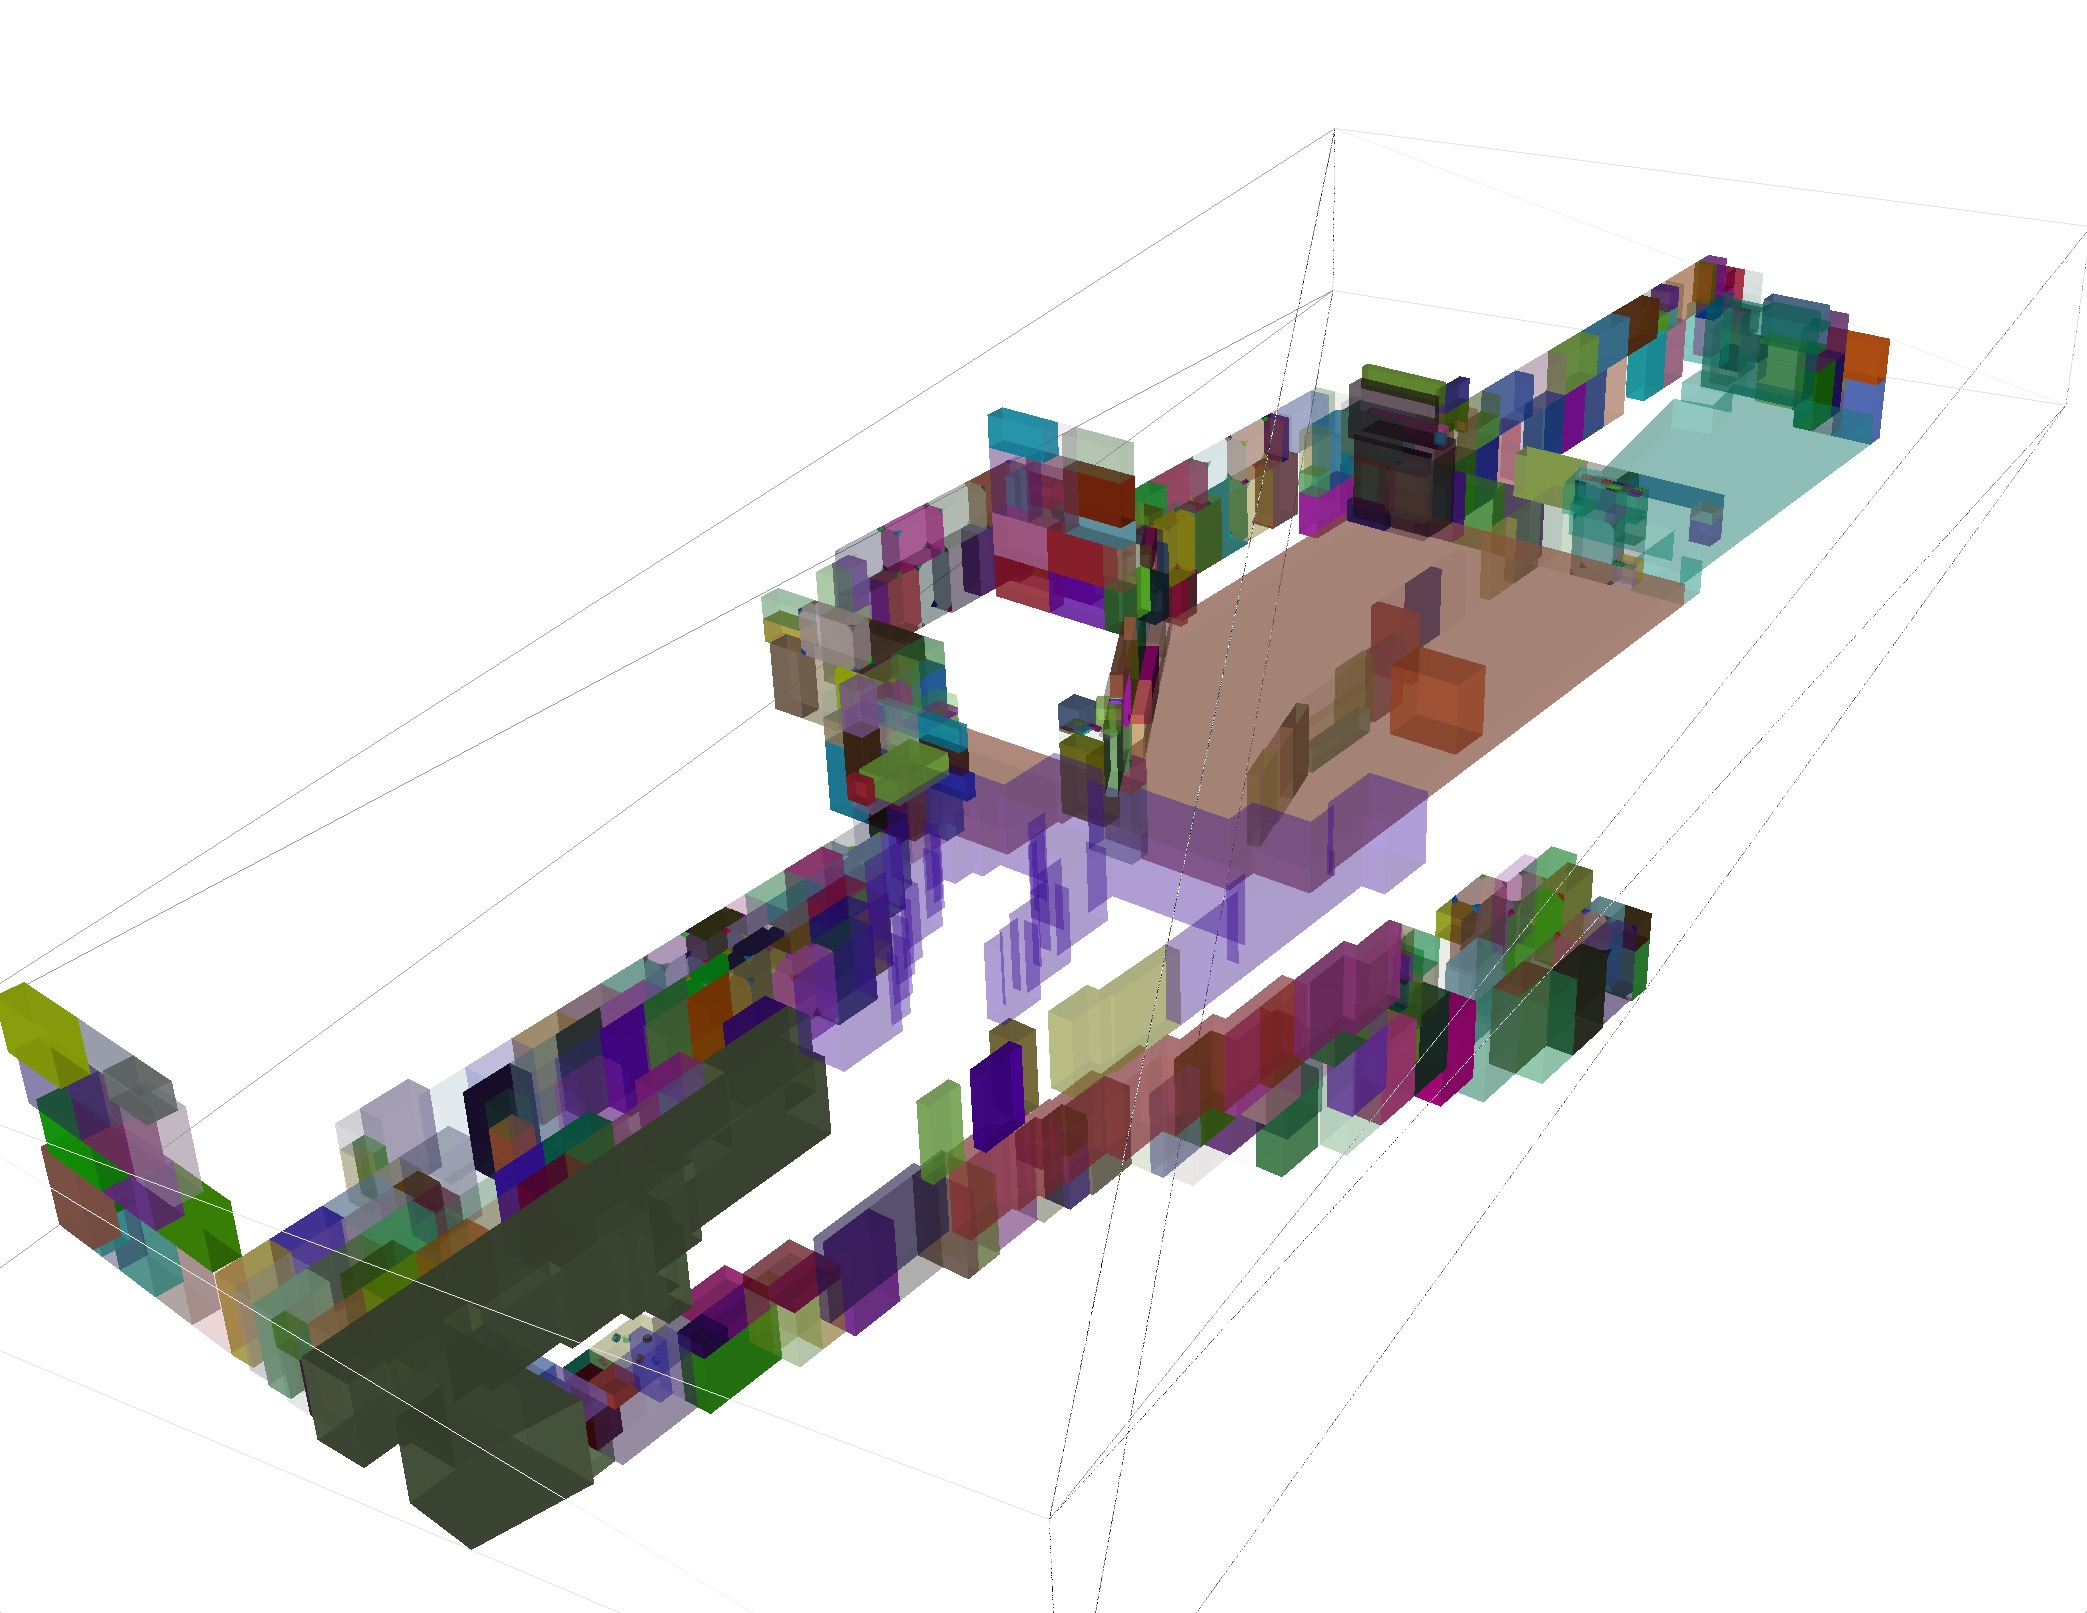
\includegraphics[scale=0.13]{Images//introduction//CernEast.jpg}
\caption[width=\columnwidth]{Converted CAD file (STEP to GDML) of the shielding at CERN East Area T8 and T11 test beam lines. Figure 4 from Source \cite{pyg4om}.}
\label{cerncad}
\end{figure}

\newpage
\noindent Figure \ref{cerncad} shows a CAD model of the shielding used in a section of CERN (or The European Organization for Nuclear Research translated from French) home to the LHC (or Large Hadron Collider). The use of particle transport simulation can also be used as a tool for simulating beam losses \cite{pyg4om}.

\subsubsection{Space Exploration}
\noindent Space exploration is also a large field where radiation transport and shielding is a key concept that must be accounted for. Beyond the Earth's atmosphere the Universe is full of harmful GCR (or Galactic Cosmic Rays) radiation making the shielding of spacecraft and astronauts a major priority. Traditionally protection against unwanted radiation has involved placing an absorber in between the target and the source. The shielding for a spacecraft is typically made from an aluminium alloy, studies have been simulated using GEANT4 (One of the software packages used in this project, detailed in Section \ref{g4}) as a way to measure its effectiveness of $Al_2O_3$ as space craft shielding \cite{spacesh}. The study specifically looks at the stopping power, which is also used later on in the project (Section \ref{stop}). 
\\\\
\noindent However for the case of astronauts the size of the required absorber is extremely large and unpractical and will likely cause showers of more harmful secondary radiation. Therefore the use of magnetic fields is being investigated as a way to divert the charged electromagnetic radiation away from a target apposed to stopping it \cite{magf}. This is something which could also be simulated in GEANT4 in the coming future, as GEANT4 has the capability to map electric \& magnetic fields \cite{bdsimpap}.

\subsubsection{Medical}
\noindent Another less obvious but essential field which radiation transport simulation is required in is medical treatment. X-ray radiation from vacuum tubes is not only used to check for fractures or breaks in bones, it also used in radiotherapy. The X-rays are used to to target unwanted growths in the body through small doses of harmful radiation, with the aim of removing cancerous tissue with minimum damage to the neighbouring organs. This can be especially difficult when the tumor is in the vicinity of organs that move within the body, such as a the lungs. As the patient needs to breath in order to live, therefore the movement of the organs needs to be accounted for when aiming the particles.
\\\\
\begin{figure}[h!]
\centering
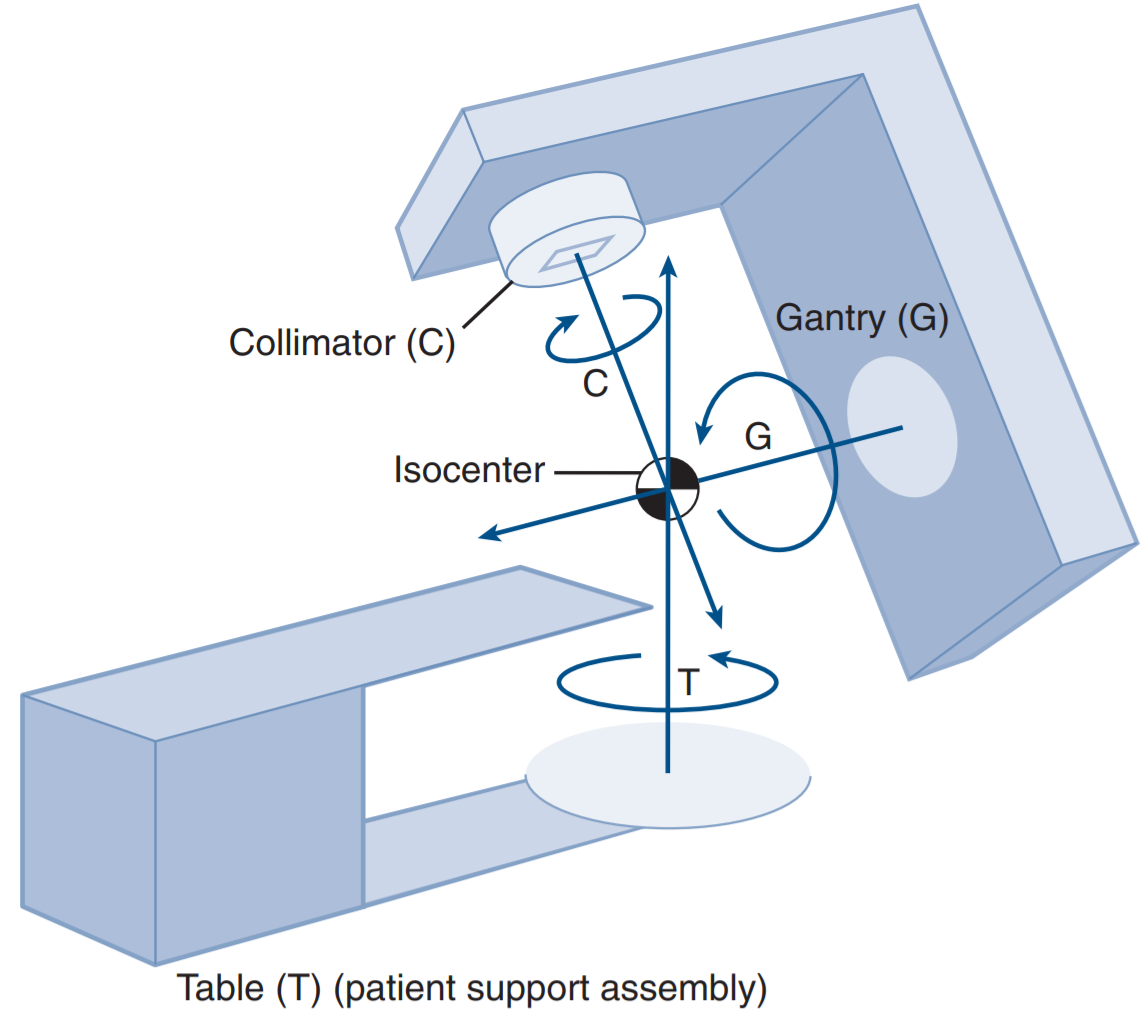
\includegraphics[scale=0.35]{Images//introduction//radiotherapy.png}
\caption[width=\columnwidth]{A diagram of a gantry-based radiation therapy machine. Figure 27.4 from Source \cite{cancer}.}
\label{cancer}
\end{figure}

\noindent A patients organs also move with the body's orientation with respect to gravity therefore the patient must be positioned laying down on a table that rotates perpendicular to the direction of gravity. The accelerator unit must then rotate around the patient to imitate the most stationary conditions. An example machine can be seen in Figure \ref{cancer}, where patients would be placed on the table to under go treatment by radiotherapy, the isocenter being the optimal target position of the cancerous cells to be in within the patents body.  A more recent type of radiotherapy that is proton therapy, which involves the use of small particle accelerators.

\subsection{Project Motivations}
\label{motiv}
\noindent Historically it has been very hard to simulate particle radiation through matter correctly, being both expensive and time consuming. As computer technology has developed through recent years particle physicists have began building models to simulate these radiation events, employing techniques such as the Monte Carlo method. Currently many independent industries all require the ability to conduct radiation transport simulations (as shown by Section \ref{back}), but work with different file formats, which is where one of the biggest problems lie. Many software tools for simulating radiation transport are format specific and require complex file conversions. Pyg4ometry is a tool created to easily convert between these representations and allow a wider audience to utilise these radiation tracking softwares. GUImesh is a similar python package for converting STEP files into GDML format \cite{meh}.

\subsection{Project Aims}
\label{aim}
Simulating radiation transport requires a description of the target 3D formation, detailing its structure, dimensions and material properties such as density. These 3D models contain elements and volumes that which can not overlap, leading to most radiation transport geometries being mad by hand.
The aims of this project are to contribute towards the optimization of the Pyg4ometry package (Section \ref{pyg}) and subsequently BDSIM (Section \ref{bdsim}), by improving parts of the code and conducting performance test to produce results that can be analysed. The main areas for improvement and where most of the computational energy in wasted, is in the meshing of the primitive GEANT4 (Section \ref{g4}) compatible solids. The inefficient computation is primarily due to the unnecessary use of boolean operations (Section \ref{bool}).
\\\\
The first part of the project and report focuses on the meshing of the primitive solids (Section \ref{prim}) within Pyg4ometry. Discussing the comparison of methods and techniques used to make not only primitive solids, but also complex compound ones. The second part of the project focuses on the performance of the meshes within BDSIM (Section \ref{int}). Investigating the effects of material and particle energy, on the duration of interactions within a solid.


% ------------------------------------------------------------------------------------------------------------------------------

\section{Types of Radiation Emission }
\label{radd}
Radiation is the transport of energy through matter or a vacuum in the form of electromagnetic waves and/or particles. There are two main categories of radiation emission; ionising and non-ionising. Non-ionising (or NIR) can be harmful if exposed to for long periods of time or in high intensities, such as UV light can cause skin cancer or shining a strong laser into an eye can cause blindness. In order for a type of radiation to be ionising it must be an electromagnetic wave or particle with enough energy to "ionise" a neighbouring atom, typically travelling at a velocity greater than 1\% the speed of light.  "Ionisation" is the process of detaching an electron from an atom or molecule. This report only focuses on forms of ionising radiation as they are the ones more commonly associated with particle interactions. 
\\\\ 
\noindent Bremsstrahlung is the electromagnetic radiation, which is typically in the form of a photon, created as the result of a charged particle decelerating after it has been deflected from another charged particle. The larger the loss in kinetic energy, i.e the greater the deceleration of the initial particle, the larger the frequency of the emitted photon. Medical X-ray tubes rely on Bremsstrahlung to create a continuously emitted spectrum. The X-ray tubes work by using an electric field to accelerate electrons within a vacuum, which is then aimed towards a target, such as a broken arm against a photographic absorber.
\\\\
\noindent Cherenkov radiation is important within nuclear reactors and is the reason why submerged reactors often appear to glow blue \cite{blue}. The blue colour is due to the radiating particles traveling faster than the speed of light in the same medium, acting in the same fashion as a sonic boom. Thus causing a continuous moving source of radiation in the visible spectrum. The blue colour is very faint and can only really appear at high energies, such as the ones found in nuclear reactors. 

% ------------------------------------------------------------------------------------------------------------------------------

\section{Software Packages}
\label{packs}
This Section goes through each package of software used throughout the duration of the project. It outlines the key details of each package, describing its function and link to the project. At the time of the project a lot of the prerequisite packages were only compatible with Linux OS  (or Operating System) and no docker images were available. Due to owning a machine that operated on windows, a lot of time was initially spent setting up virtual machines running Cent0s 7 (standard free Linux OS used by CERN \cite{cern}). However despite getting it setup, the packages were not performing to the same standard as they were on the fellow Apple MacBooks. Therefore for the main duration of project, a Linux laptop was loaned out from the particle physics department of Royal Holloway (a 2011 Apple MacBook Pro running OS El Capitan). This legacy operating system came pre-installed with the some of the required packages, and allowed for easy installation of outstanding backdated versions. 

\subsection{Pyg4ometry}
\label{pyg}
Pyg4ometry is an open-source Python package  written by the John Adams Institute (JAI) \cite{jai}, its purpose is to convert 3D CAD (Computer Aided Design) geometries between different representations to allow compatibility with BDSIM (Section \ref{bdsim}) for the simulation of radiation transport \cite{pyg4om}. The ``4'' in ``Pyg4ometry'' comes from the consistency the package has with GEANT4 (Section \ref{GEANT4}). The package is a key tool for allowing multiple file formats, such as STEP/STL or IGES files to be converted into GDML files, which are the compatible format for BDSIM. GDML (or Geometry Description Markup Language) is a format based on XML files. The range of file compatibility increases the number of people who can utilise both Pyg4ometry and BDSIM, as many industries use different file formats to store their 3D CAD geometries.
\\\\
\noindent Pyg4ometry can also be used to determine if a model has any geometric overlaps. As well as making loading CAD geometries into BDSIM much faster than using the full GEANT4 C++ application, as well as fast VTK visualisation discussed in Section \ref{vis}. Most of the development in this project is conducted in Pyg4ometry and managed using an online BitBucket code repository \cite{bitb} in combination with Sourcetree \cite{st} (An open-source git management GUI). As of January 2020 the first CentOs 7 docker image for Pyg4ometry is now available in the source code repository. The package is currently written in and only supports Python 2.7, however as of January 2020 support for Python 2 has been discontinued as the newer version Python 3 is taking over. The transition to Python 3 means adjusting the syntax of several functions and files in Pyg4ometry, this has began, but a full transition will take sometime as it is not an immediate priority. 

\subsection{GEANT4}\label{GEANT4}
\label{g4}
GEANT4 (or GEometry ANd Tracking) is a software developed in C++ for the simulation and tracking of particles traveling through matter by employing the Monte Carlo method (Section \ref{monte}). The package is used by many particle physicists and is one of the more popular geometry handling packages for interactions. GEANT4 has its own preset primitive solids that are used for simulating particle interactions and can be found within the online manual \cite{solids}. For ease of conversion between file formats Pyg4ometry uses the same conventions when meshing its primitive solids. GEANT4 has a large inbuilt database which contains the properties of most materials and particles. GEANT4 is often referred to as a particle transport code, an alternative transport code is FLUKA (or FLUktuierende KAskade), which also uses Monte Carlo to simulate high energy physics. Pyg4ometry is also developing compatibility with other transport codes such as FLUKA, MCMPX, MAD and Transport \cite{pyg4om}. GEANT4 can and has also been used to conduct dose calculations for radiotherapy patients \cite{dose}.
\\\\
The materials used in Pyg4ometry and throughout this project are also from the GEANT4 database \cite{mater}. In this report the three main materials used are $G4\_Fe$, $G4\_Ti$ and $G4\_Galactic$ (Iron,Titanium and Vacuum). The use of $G4\_Galactic$ is arguably the most important as it is used to set the material of the world environment in which other objects are placed into. By default the world material in BDSIM is set to be air, which means the particles would interact before passing into the object being tested, this was avoided by using the option $worldMaterial=``G4\_Galactic"$ within the GMAD files. Other properties for each GEANT4 material are also used in this project, such as the stopping power (Section \ref{stop}). 

\subsection{BDSIM}
\label{bdsim}
BDSIM (or Beam Delivery SIMulation) is an open-source software package also written by JAI, for the use of modelling particle beam interactions. The pacakge has many applications, such as modelling complex particle accelerators like the LHC (or Large Hadron Collider) or concepts magnets for medical scanners used to treat tumours. G4Beamline \cite{g4beam} is a similar package, however includes the effects between particles ('collective effects') , which BDSIM does not due to better tracking and geometry in general. Both BDSIM and G4Beamline alike use GEANT4 as a basis for their beamline simulations. BDSIM allows a user to specify the physics being used for a particular particle interaction, such as the particle energy and the number of secondaries produced. The scattering of the particle trajectories and decays are computed using Geant4's Monte Carlo calculations, to make the results as consistent with experimental results as possible. The software outputs a full analysis of each run, and can even allow multiple runs to execute at once (batch mode).
\subsubsection{PyBDSIM}
\label{pyb}
BDSIM has a Python library called PyBDSIM which allows interactions to be automated and analysed using Python scripts. PyBDSIM also allows for the navigation of ROOT analysis files to extract data to plot, mentioned more in Section \ref{root}. This is how all the plots in Sections \ref{prim} \& \ref{int} are generated.

\subsection{ROOT}\label{root}
ROOT is not an acronym and is named after the idea, that it is a system for other systems to grow off of, much like a root of a tree that has many branches. ROOT is adopted by many physics communities such as CERN \cite{cern}, where it was first written. Naturally making it a popular format for particle physicists in particular and is the why it is the default output for analysis by BDSIM. ROOT has its own GUI for file browsing. called a ``TBrowser'', due to the nature of its formatting. Despite ROOT generating its own plots, no ROOT files or plots are shown in the report, as the data has been extracted from the root files and replotted using PyBDSIM \ref{pyb} and Matplotlib (library for creating publication grade figures). The plots are made this way as the data can be more easily manipulated and the formatting of ROOT plots is unpopular.

\subsection{Freecad}
In this report the libraries from Freecad 0.18 \cite{18} are used directly within Pyg4ometry (Section \ref{pyg}), without the use of the Freecad GUI (or Graphical User Interface). The libraries are used to import STEP (Standard for The Exchange of Product data) files and to convert them into triangular based tessellated meshed solids, that can then be written out as a GDML file. As an exercise at the beginning of the project a few example CAD STEP files were downloaded from the internet and converted into meshed GDML files. One of the CAD models converted was a GPS satellite, which can be seen in Figure \ref{sat}. Freecad itself can also be used to create CAD models that can then be tested in BDSIM, example magnet shown in Appendix \ref{mag}.

\subsection{Visualisation}
\label{vis}
Most of the packages mentioned above have their own GUI's to visualise the meshed geometries. However the main two GUI's used in this project are the ones connected with Pyg4ometry and BDSIM. VTK (or Visualization ToolKit) is an open-source software for displaying and manipulating scientific data \cite{vtk}. Pyg4ometry uses VTK, shown in Figure \ref{sat}, to create its 3D interactive GUI. BDSIM uses GEANT4's GUI (as seen in Figure \ref{screengrab}), which is another reason Pyg4ometry aims to be consistent with GEANT4. Both the VTK and GEANT4 GUI's allow meshed solids to be viewed as solids or as meshed structures. The GEANT4 GUI has its own console in which commands can be carried out, allowing interactions to be altered from within the GUI as well as by PyBDSIM.

\begin{figure}[h!]
\centering
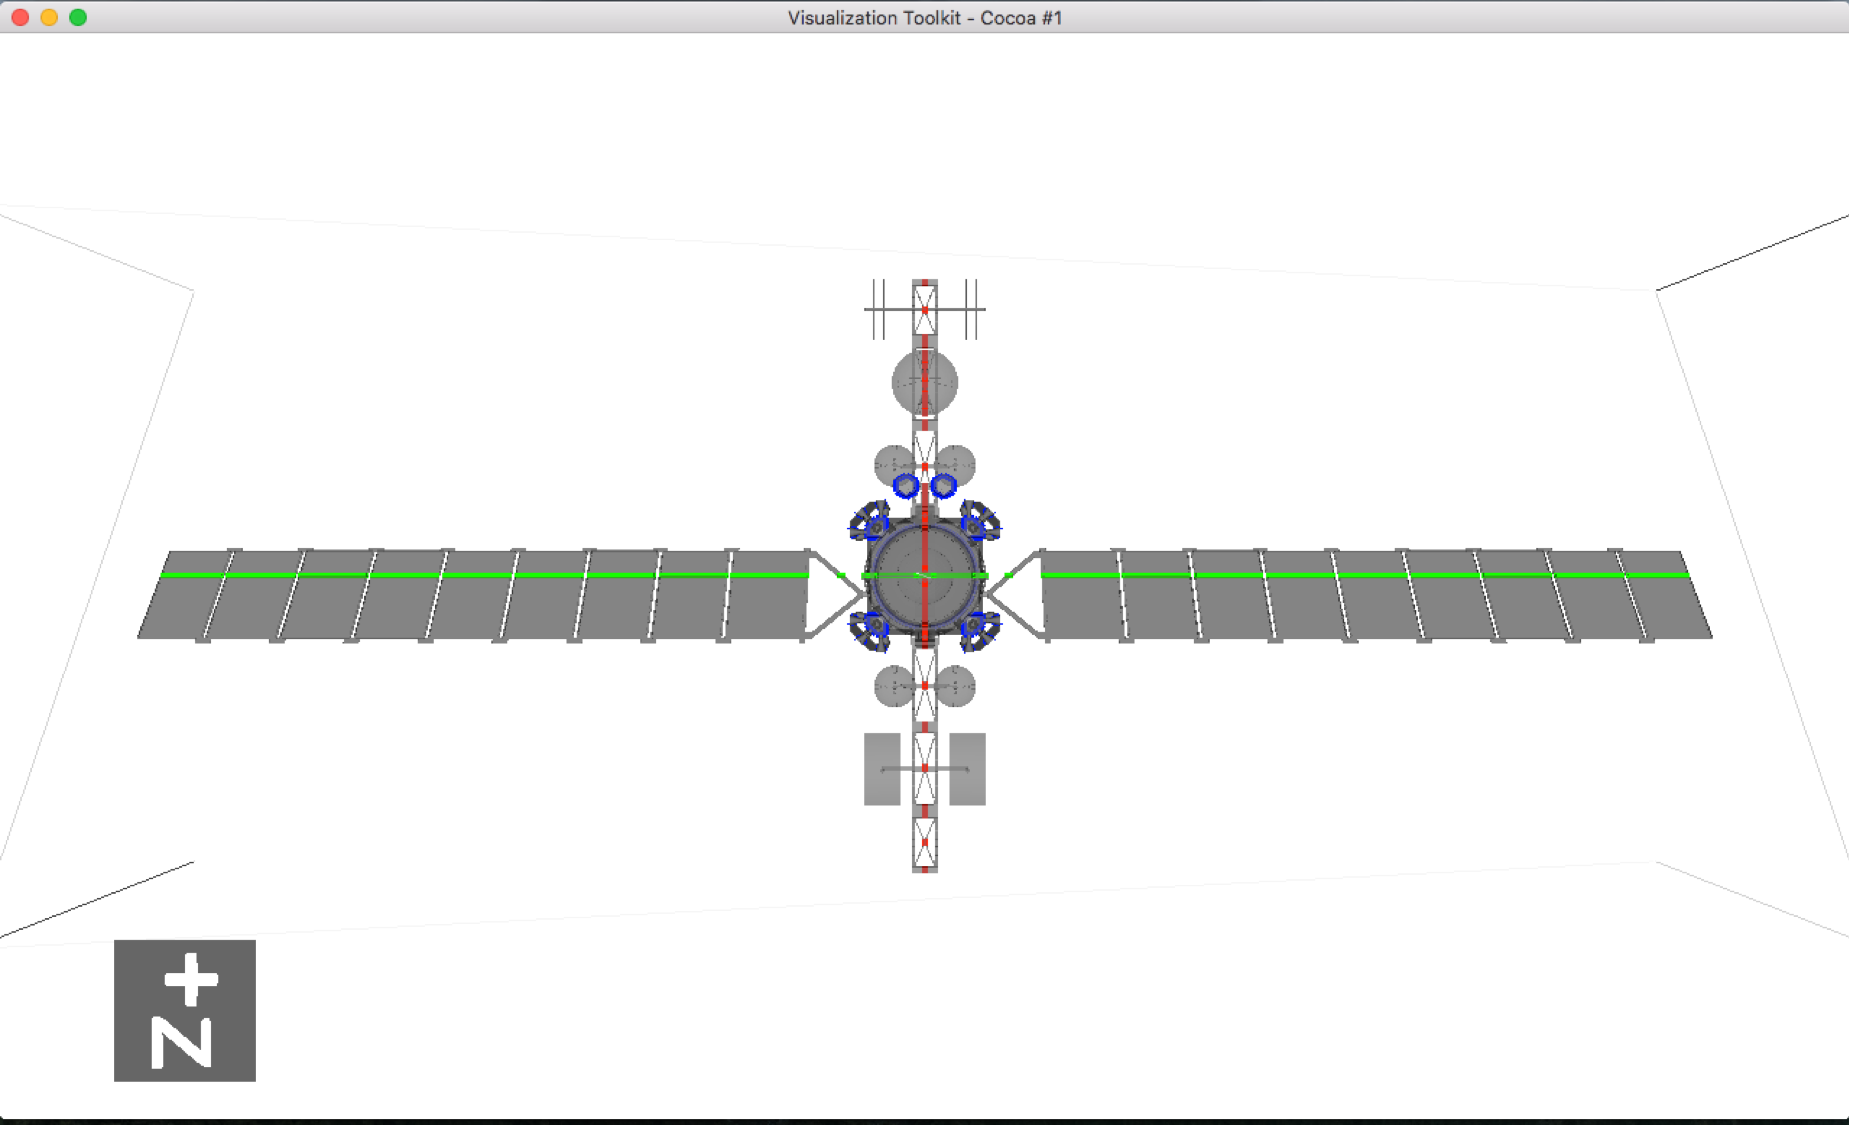
\includegraphics[scale=0.4]{Images//VTK/sat.png}
\caption[width=\columnwidth]{STEP file of a GPS satellite imported into Pyg4ometry using the Freecad libraries and viewed in VTK. Original STEP file from Source \cite{sat}.}
\label{sat}
\end{figure}

\begin{figure}[h!]
\centering
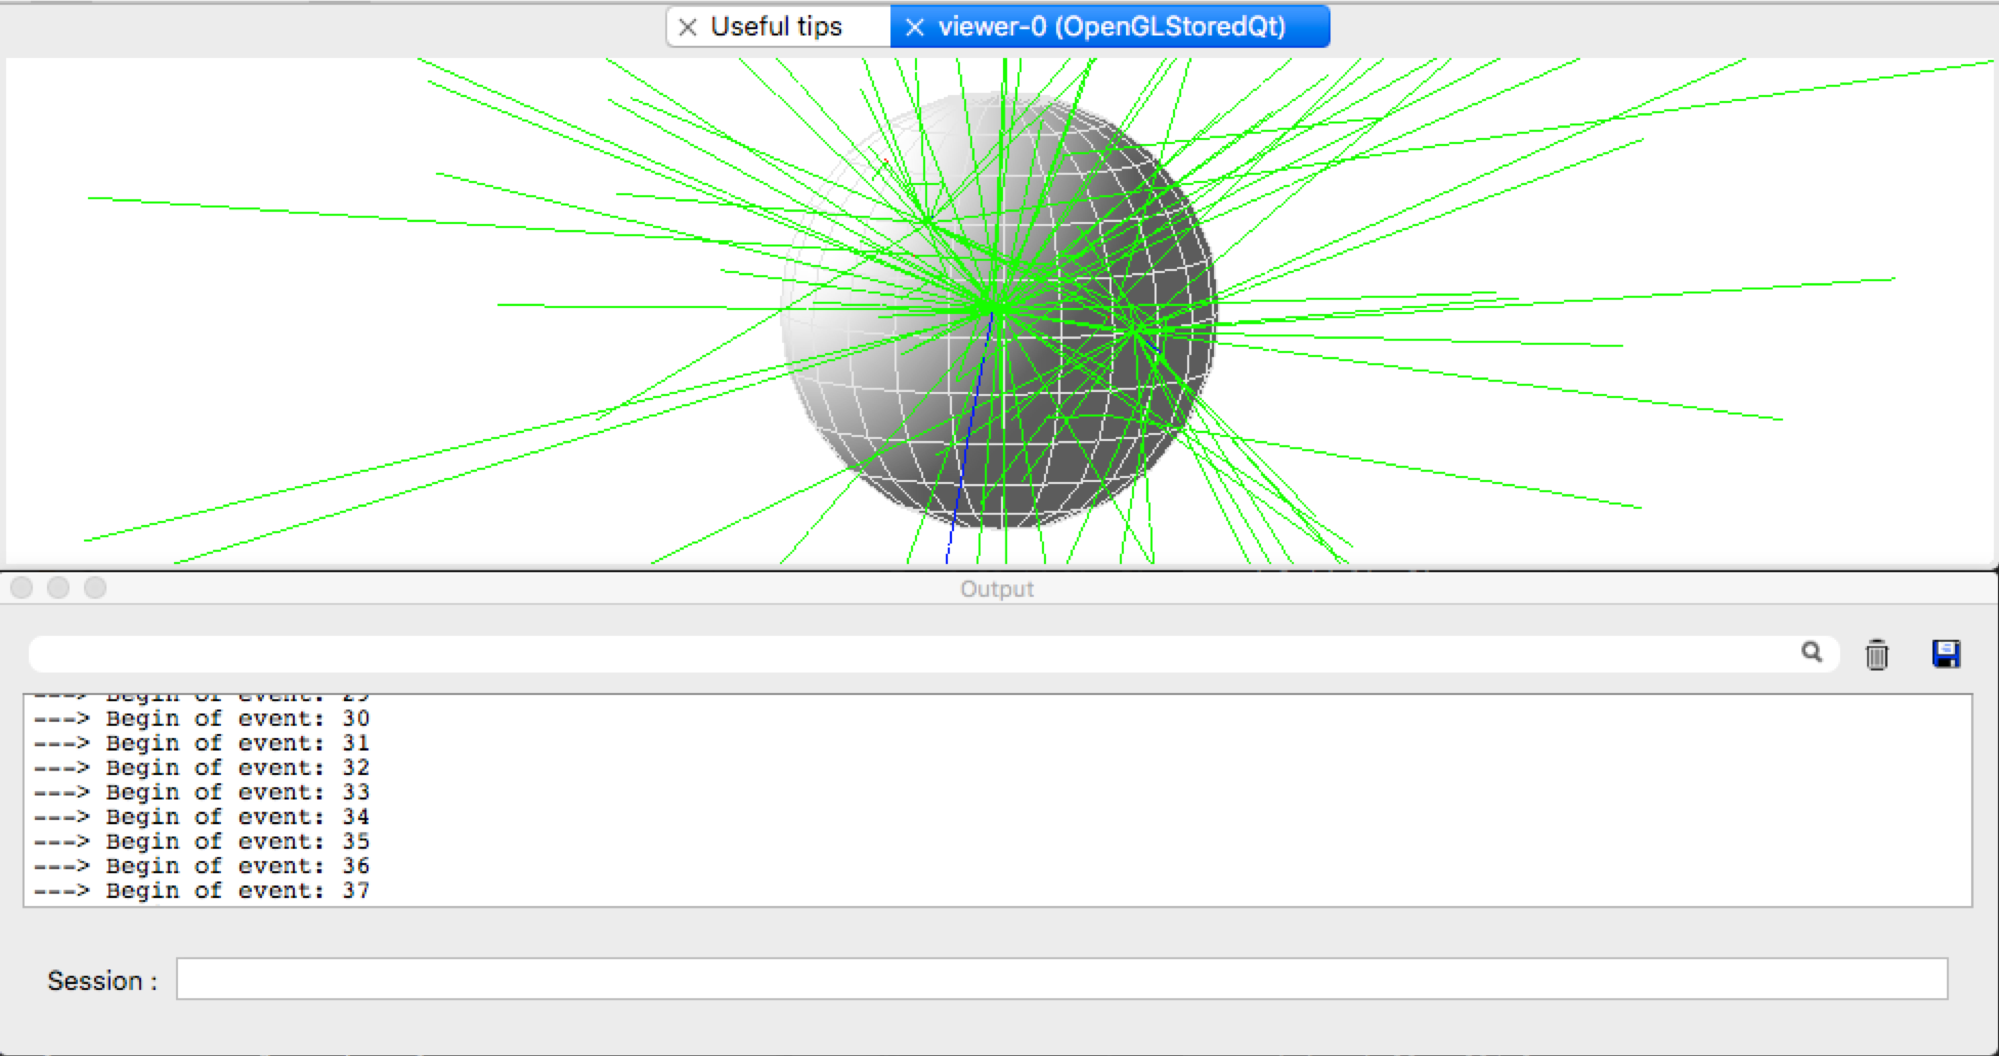
\includegraphics[scale=0.4]{Images//BDSIM//screengrab.png}
\caption[width=\columnwidth]{BDSIM GUI screenshot of a 3D particle interaction and output window. Interaction involving a GEANT4 sphere with 10,000 1.3 GeV neutrons.}
\label{screengrab}
\end{figure}


% ------------------------------------------------------------------------------------------------------------------------------
\newpage
\section{Primitive Meshing}
\label{prim}
This section will describe the work done to optimize the Python scripts that generate the three dimensional meshings for the primitive solids within the Pyg4ometry package (Section \ref{pyg}). All the primitive solids used are constructed such that they are compatible with GEANT4's solids \cite{solids}. It was previously thought that it would be best to use purely triangular based meshes in combination with boolean operations to construct the 3D solids. As the triangle is the shape which has the minimum amount of points needed to define a planar face containing an area. Prior to the project it had been realised that the computation of triangles and boolean operations in most cases is much more intensive and inefficient, compared with the polygons and adapted trigonometry. In particular with the curved solids are the most computationally heavy, i.e cylindrical, spherical and toroidal based solids, due to the boolean operations generating more complex meshes. Thus the first part of the major project was to rewrite the meshing scripts for all the curved primitive solids in Pyg4ometry (Section\ref{pyg}).
\\\\
One of the major improvements to the Pyg4ometry meshing scripts was in the computation of cut up primitive solids. The meshing of hollow or sliced solids were previously constructed by boolean subtractions and intersections, which involves using two or more separate solids and operating on them to create a final single solid. Discussed more in Section \ref{bool}. Which resulted in a very computationally heavy and less aesthetic outcome, where the mesh lines (``slice and stack'') were often meshed in non-axial directions.

\subsection{Co-ordinate Systems}
\label{cosy}
The various primitive solids are all constructed by using the predefined parameters used by GEANT4, to be consistent with GEANT4's own convention for solids. The parameters defining a 3D solid are properties relating to the co-ordinate system that the solid is constructed within. For example for a simple cylinder the parameters would be a height and radius. The parameters are then used to generate points on the object via basic trigonometry. The points can then be used as vertexes to define faces on the given solid. The number of faces and subsequently the number of points on a solids surface defines the mesh density. The order in which the points are appended is also very important and is detailed in Section \ref{order}.
\\\\

\begin{lstlisting}[language=Python, label=code1, caption=Basic Python function structure for new meshing of primitive solid in Pyg4ometry.]
def pycsgmesh(nslice,nstack, *args, **kwargs):

    # ... 
    
    polygons = []

    for j0 in range(nslice):
        j1 = j0
        j2 = j0 + 1
    
        vertices = []

        for i0 in range(nstack):
              i1 = i0
              i2 = i0 + 1     
              
    #....
    
    return mesh

\end{lstlisting}


\noindent The Python meshing scripts for all co-ordinate systems follow a similar structure, using a pycsgmesh() function, the beginning of which can be seen in Listing \ref{code1}. The ``CSG'' in ``pycsg'' stands for Constructive Solid Geometry, which is a  modeling technique that uses Boolean operations to construct 3D solids. The naming convention is left over from when the old meshing scripts employed boolean operations. The script works by  first defining an empty list of faces (polygons) and then running the associated trigonometric equations through a number of loops to generate and append polygons to that list. The number of loops is associated with the number of sections a surface of a solid is being split up into in a given co-ordinate system (``nslice'' \& ``nstack'' in Listing \ref{code1}). The two parts of Listing \ref{code1} where code has been commented out is where a lot of repetitive code is placed. The first comment block is where the units and other empty lists are defined and the second is were all the points, faces and polygons are constructed using ``pycsg.geom'' functions. The density of the mesh is defined by the user inputted number of slices and stacks, of which the orientation varies with co-ordinate system. The slice and stack used by the new meshing scripts for the solids in the cylindrical polar, spherical \& toroidal co-ordinate systems are demonstrated in Figures \ref{cylmeshin}, \ref{sphmeshin} \& \ref{tormeshin}.

\subsubsection{Cylindrical Polar Co-ordinate System}
\label{cycl}
In the cylindrical polar co-ordinate system the loops within the equivalent function to Listing \ref{code1}, creates 3 or 4 points at a time using an adaptation to the trigonometry in Equations \ref{cyctrig}, which can then be used to define a triangular or quadrilateral face. The only cases where the new meshing produces triangles is at the top and bottom faces of the cylinder. These cases are only true provided the solid does not have a minimum radius equal to zero (creating a tube or cone). The same logic for the triangular faces is identical to that of the quadrilateral faces, just using 3 vertex points to make a face.

\begin{figure}[h!]
\centering
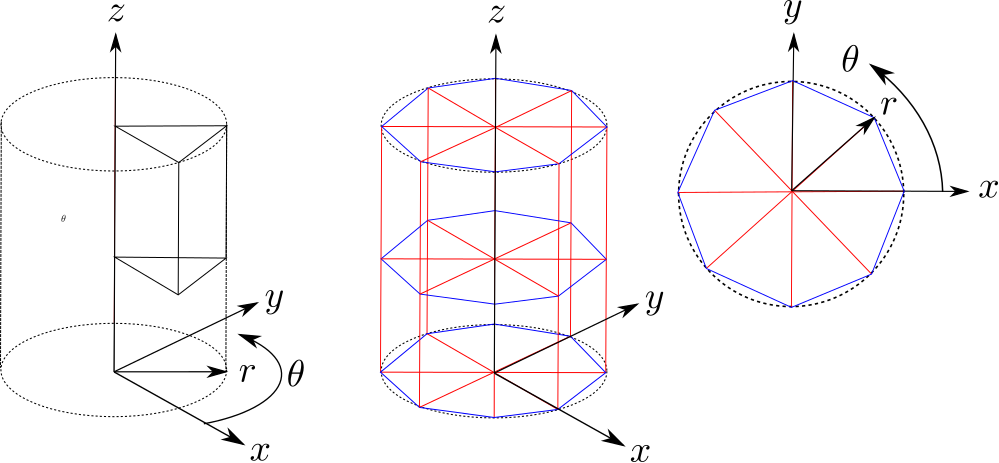
\includegraphics[scale=0.45]{Images//Coords//cyl.png}
\caption[width=\columnwidth]{A diagram showing the meshing method for a cylindrical polar co-ordinate system, where the red lines indicate the slices (8) and the blue indicate the stacks (2). The diagram was drawn using the CAD software Inkscape.}
\label{cylmeshin}
\end{figure}
The trigonometry that converts the points from cylindrical polar co-ordinates to Cartesian, are:
\begin{equation}
\begin{aligned}
\label{cyctrig}
& x = r \cos{\theta} \\
& y = r \sin{\theta} \\
& z = z
\end{aligned}
\end{equation}

\noindent The only time a stack is needed in the cylindrical co-ordinate system is when the solid has a non-linear function in the r-z plane. For example a paraboloid (Figure \ref{paraco}) would need a stack, but a linear cone (Figure \ref{consco}) would not. This is due to the fact that a singular plane can not represent a curved surface with a one face. 

\begin{figure}[h!]
\centering
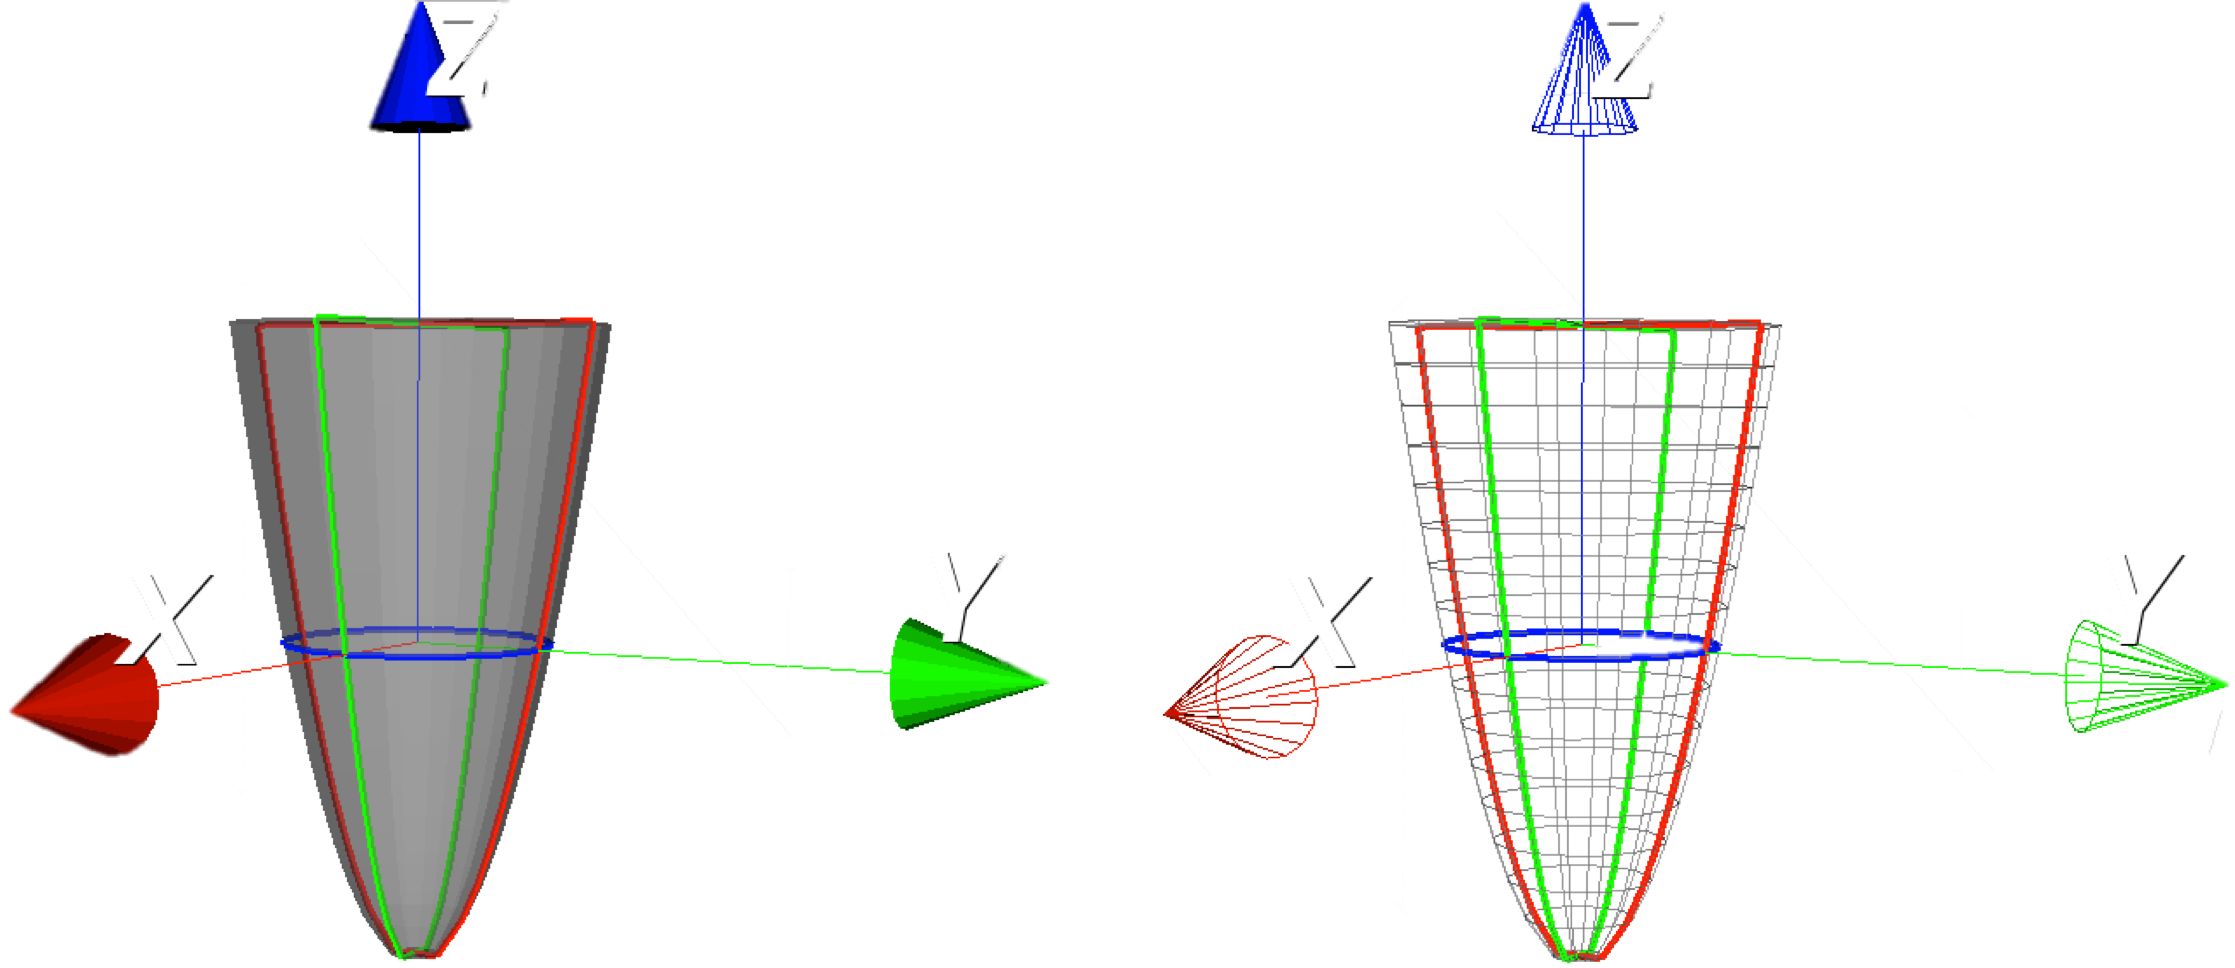
\includegraphics[scale=0.3]{Images//Coords//para.png}
\caption[width=\columnwidth]{A VTK screenshot of a paraboloid constructed using the new meshing method in cylindrical polar co-ordinate system, where the red lines indicate the points residing on the x=0 plane, the blue lines indicate points on the z=0 plane and green lines indicate points on the y=0 plane.}
\label{paraco}
\end{figure}

\begin{figure}[h!]
\centering
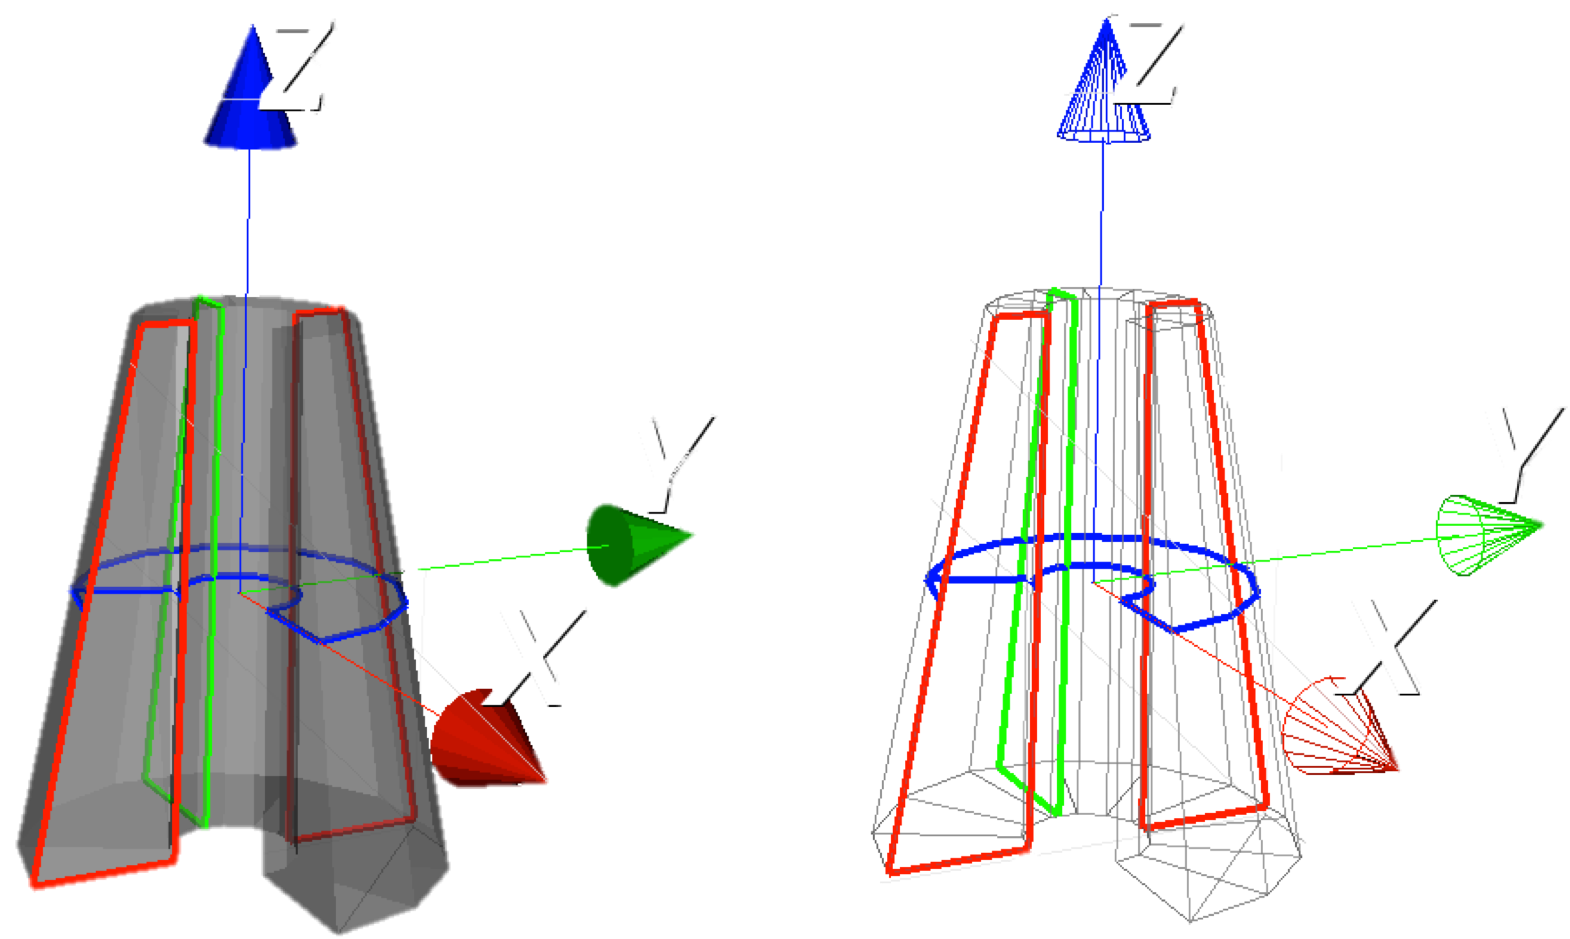
\includegraphics[scale=0.3]{Images//Coords//consco.png}
\caption[width=\columnwidth]{A VTK screenshot of Cons constructed using the new meshing method in cylindrical polar co-ordinate system, where the red lines indicate the points residing on the x=0 plane, the blue lines indicate points on the z=0 plane and green lines indicate points on the y=0 plane.}
\label{consco}
\end{figure}


\subsubsection{Spherical Co-ordinate System}

The meshing for the primitive solids in spherical co-ordinate systems are constructed by similar means the that of the cylindrical. Just with different trigonometric equations (Equations \ref{trigsph}) as a result of two angle parameters $\phi$ and $\theta$. The stack (blue) and slice (red) for solids in the spherical co-ordinate system works in the same way as the longitudinal and latitudinal mapping on a globe, shown in Figure \ref{sphmeshin}. 
\\\\
The trigonometry that converts the points from spherical co-ordinates to Cartesian, are:

\begin{equation}
\begin{aligned}
& x = r \cos{\theta}\sin{\phi}\\
& y = r \sin{\theta}\sin{\phi} \\
& z = z
\end{aligned}
\label{trigsph}
\end{equation}
\begin{figure}[h!]
\centering
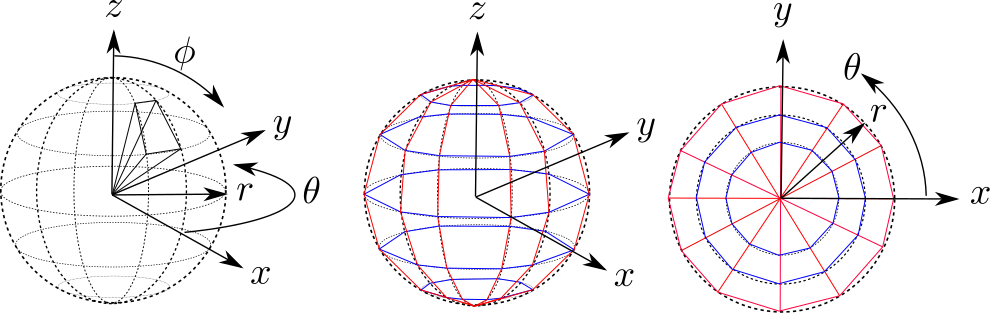
\includegraphics[scale=0.5]{Images//Coords//sph.png}
\caption[width=\columnwidth]{A diagram showing the meshing method for a spherical co-ordinate system, where the red lines indicate the slices (12) and the blue indicate the stacks (6). The diagram was drawn using the CAD software Inkscape.}
\label{sphmeshin}
\end{figure}

\noindent The structure of the code for a spherical system is the same as used in Listing \ref{code1}. The only time triangles are constructed in the spherical co-ordinate system is if a complete pole exists at the top or bottom of the solid. The solids constructed in the spherical co-ordinate system always have both a stack and a slice.

%\begin{lstlisting}[language=Python, caption=Python example]
%for j0 in range(nslice):
%    j1 = j0
%    j2 = j0 + 1
%
%    for i0 in range(nstack):
%          i1 = i0
%          i2 = i0 + 1
%\end{lstlisting}

\newpage
\subsubsection{Toroidal Co-ordinate System}

The toroidal co-ordinate system is a special case and is only needed, for toroidal based solids. The stack and slice for a toroidal shape is much harder to visualise, due to the fact it is a rotating co-ordinate system. A toroidal slice is an $R_{Torus}$ radial cut taken out of the angle $\phi$ and a toroidal stack is a $R$ radial cut out of the angle $\theta$, where the angles and radii are displayed in Figure \ref{tormeshin}. 
\\\\
The trigonometry that converts the points from toroidal co-ordinates to Cartesian, are:

\begin{equation}
\begin{aligned}
& x = R_{Torus} + R\cos{\theta}\cos{\phi} \\
& y = R_{Torus} + R\cos{\theta}\sin{\phi} \\
& z =  R\sin{\theta} 
\end{aligned}
\end{equation}

\begin{figure}[h!]
\centering
\includegraphics[scale=0.35]{Images//Coords/torus_coords.png}
\caption[width=\columnwidth]{Diagram showing the meshing method for a toroidal co-ordinate system. Diagram drawn using the CAD software Inkscape.}
\label{tormeshin}
\end{figure}

\subsection{Plane Direction}
\label{order}
A key thing to be taken into account when writing Pyg4ometry meshing scripts is the order convention being used for appending points/vertexes to a list, to define a plane, i.e to define a face on a solid. This is important as the direction the normal of the plane points in, dictates whether a face is considered an inside or outside face on the given solid. Getting this order incorrect, will lead to missing faces, when the meshing is made.

\begin{figure}[h!]
\centering
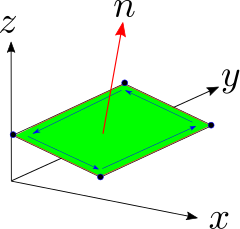
\includegraphics[scale=0.7]{Images//append_points//Point_Appending_Order.png}
\caption[width=\columnwidth]{A diagram showing the order convention of appending points to define the normal to a plane. The diagram was drawn using the CAD software Inkscape.}
\label{pointsorder}
\end{figure}
\noindent The convention is that the normal to a plane points away from the solids surface, making it an exterior face. The normal is in the z direction to a plane residing on z=0, if the points are appended anticlockwise in the x-y plane. For points appending in the other direction (clockwise in the x-y plane), the normal would be in the -z direction, making an interior face. The concept is shown in Figure \ref{pointsorder}.
\\\\
The simplest way to test this is by performing boolean operations with a solid box, as the boolean operation will only work correctly if all the planes are correct on both shapes, mentioned in more detail in Section \ref{bool}. This test only works for the visualiser in BDSIM as it uses GEANT4, which displays face directions. VTK inside Pyg4ometry is a much more lenient visualiser and will display solids even if their normals are incorrect, giving you a false perspective of what is being displayed.

\subsection{New Meshing of Curved Primitive Solids}
In total there are 12 curved primitive solids, of which many of the examples and concepts are very similar. Therefore only a few select solids will be discussed in this section, but the remaining solids and their development can all be viewed in Appendix \ref{app1}. The naming convention of the solids being used in this project and within this report are the ones used by GEANT4.
\\\\
One of the curved solids for which the meshing was rewritten is the hyperboloid, the old and new meshing structures of the hyperboloid is shown in Figure \ref{polypic1}. It can be seen that in this example the meshing at the top and bottom faces becomes more radially uniform. This is due to the replacement of boolean subtractions with simple trigonometry within the new meshing algorithm for the polycone.
\\\\

\begin{figure}[h!]
\centering
\begin{minipage}{.4\textwidth}
  \centering
  \includegraphics[height=1\linewidth]{Images//Meshes//Hyperboloid.png}
  \captionof{figure}{VTK screenshots of\\ hyperboloid meshing Development\\ (Solid \& Mesh View)}
  \label{polypic1}
\end{minipage}%
\hspace{1mm}
\begin{minipage}{.4\textwidth}
  \centering
  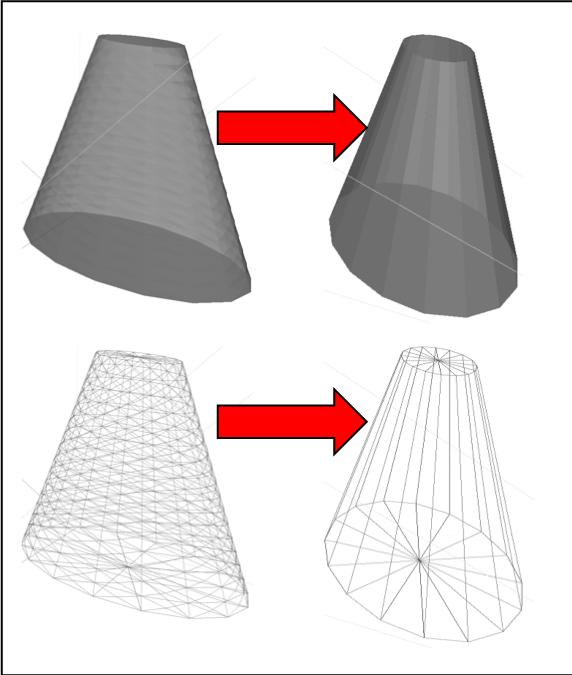
\includegraphics[height=1\linewidth]{Images//Meshes//ellipticalcone.png}
  \captionof{figure}{VTK screenshots of\\ ellipticalcone meshing Development\\ (Solid \& Mesh View)}
  \label{elco1}
\end{minipage}%
\end{figure}

\noindent Another curved solid that was remeshed is the ellipticalcone, as seen in Figure \ref{elco1}. Despite having no boolean operations to generate this solid, the meshing is still improved by replacing all the unnecessary triangular faces with quadrilateral ones. For the ellipticalcone it was also possible for the stack to be removed, as for a cone the faces in the r-z plane (in cylindrical co-ordinates) are a linear function.
\\\\
\noindent A feature that is also removed by the transition to the new meshing algorithms is the "grenade like" texture seen on the surfaces of the curved solids. The clearest example being the ellipsoid, shown in Figure \ref{ellipme}, where it can be seen that the surface of the solid has not only become triangulated, but also has a contour. This is due to the fact that the old mesh would tend to use quadrilateral based pyramids instead of quadrilateral faces in attempt to better estimate a true curved solid. This was done by rotating every other stack to be out of phase when appending vertexes. Despite this improving the mesh accuracy, it was removed as when you increase the orders of stack and slice to high enough orders the difference is negligible and is not worth the extra computation.  

\begin{figure}[h!]
\centering
\includegraphics[scale=0.6]{Images//Meshes//Ellipsoid.png}
\caption[width=\columnwidth]{VTK screenshots of ellipsoid meshing Development (Solid \& Mesh View)}
\label{ellipme}
\end{figure}

\subsubsection{Degenerate Points}
Degenerate points are another common mistake which can cause missing faces to occur, due to creating a face with null area. Multiple meshing points occupying the same point in space can spring a few errors, sometimes without entirely crashing the meshing script, making it a potentially hard error to identify. It is typically given away when a $DivisionByZero$ error occurs, within the pycsg meshing of a solid. You can identify whether this is the error by debugging each polygon and triangle in a mesh, looking out for a face that has two or more vertices with the same $(x,y,z)$ coordinates. This typically happens when you intend to mesh a triangle, but are still using the format for meshing a quadrilateral face. Or it can be due to the incorrect choice of an incorrect stack and slice iteration when constructing a face, as mentioned before in Section \ref{cosy}.

\subsubsection{Boolean Operations}
\label{bool}
\begin{figure}[h!]
\centering
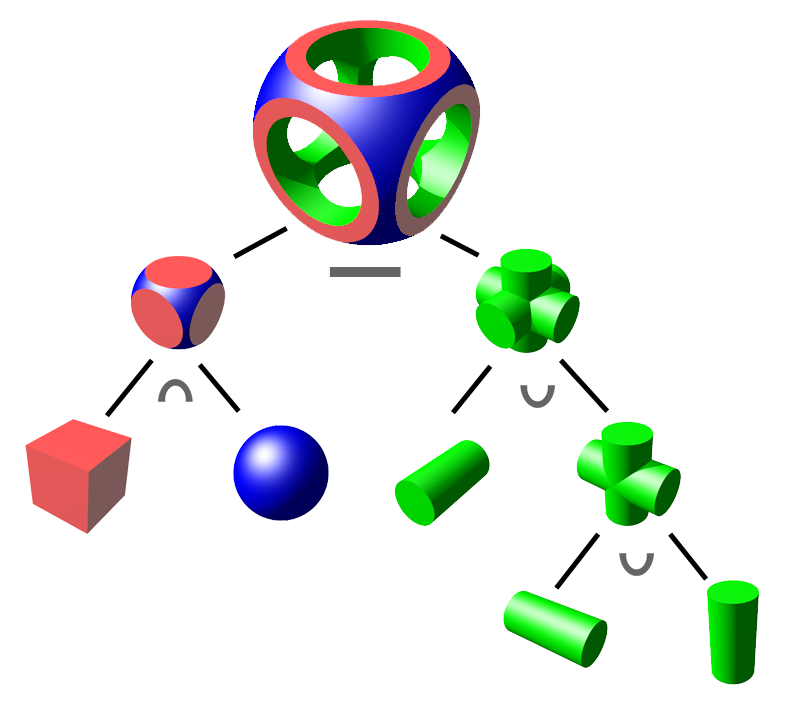
\includegraphics[scale=0.25]{Images//Booleans//Boolean.png}
\caption[width=\columnwidth]{An example CSG showing the basic method of constructing a more complicated 3D solid out of boolean operations with simpler primitive solids.\\
Where - = Boolean Subtraction, n = Boolean Intersection, u = Boolean Unions.}
\label{booly}
\end{figure}

One of the largest improvements to the performance of the new meshing methods compared with the previous methods, is the discarding of boolean operations in order to create hollow or cut-up primitive solids. The idea can be clearly seen in Figure \ref{booly}, where you conduct basic operations on simple solids, resulting in a more complex solid being made.
\\\\
\noindent Figures \ref{uni} \& \ref{sub} are of the meshed boolean union and subtraction of a solid box with a hollow sphere (in solid view). The coloured lines are representing the perpendicular planes to the axes in which the final object is placed in. These were made in the process of checking the normals before passing them into BDSIM to undergo particle interactions.
\\
\begin{figure}[h!]
\centering
\begin{minipage}{.4\textwidth}
  \centering
  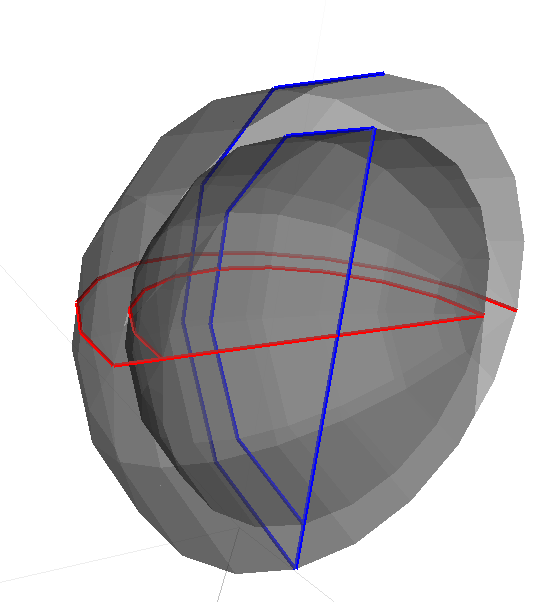
\includegraphics[height=0.5\linewidth]{Images//Booleans/SphereUnion.png}
  \captionof{figure}{Example screenshot of\\ a Boolean Union produced in\\ Pyg4ometry \& viewed in VTK.}
  \label{uni}
\end{minipage}%
\begin{minipage}{.4\textwidth}
  \centering
  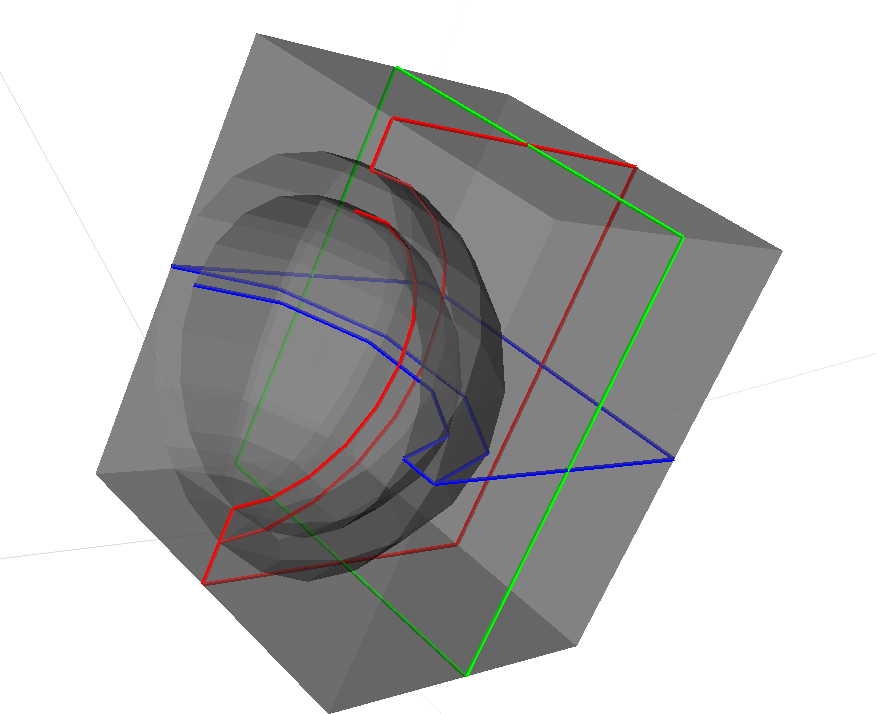
\includegraphics[height=0.5\linewidth]{Images//Booleans//SphereSubtraction.png}
  \captionof{figure}{Example screenshot of \\ a Boolean Subtraction produced\\ in Pyg4ometry \& viewed in VTK.}
  \label{sub}
\end{minipage}%
\end{figure}

\noindent The old meshing algorithms heavily relied on these operations, using intersections to slice solids and subtractions to make solids hollow or cut-up. For example CutTubs, as seen in Figure \ref{ct}, is made from two cylinders and a rotated Box, first the two cylinders were subtracted from one another, creating regular Tubs (as seen in Appendix Figure \ref{ctub}). The hollowed out cylinder was then intersected with the the tilted box to create angled tips. This has now all been replaced with clean trigonometry.
\\\\\\
The appearance of the mesh structure itself is also affected by the use of boolean operations, the boolean operations worked by trying to identify common mesh points then remesh. This created a lot of non-radially uniform mesh sections as seen in solids such as the hyperboloid, mentioned before in Figure \ref{polypic1}, in which the new meshing algorithm outputs clean radial faces at for the top and bottom sides of the solid.
\\\\
In summary As proven by the above examples the boolean operations worked, however are very computationally heavy compared with that of the adapted trigonometry that is implemented in the new method. This is the case especially when one or more of the orginal solids is curved in structure.

\begin{figure}[h!]
\centering
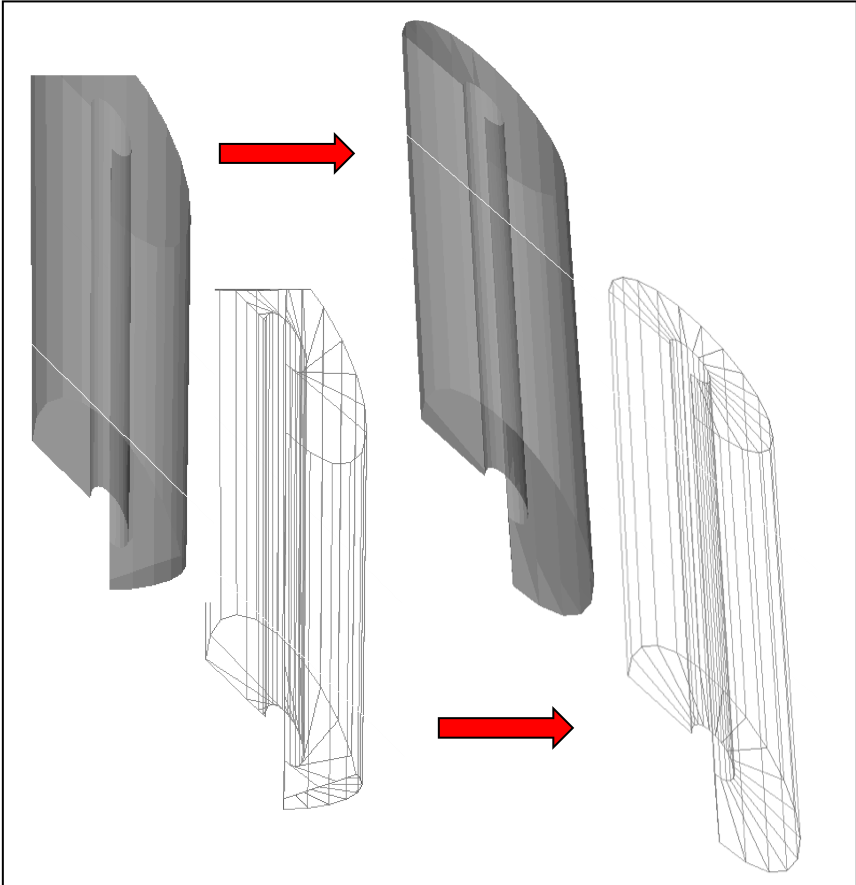
\includegraphics[scale=0.5]{Images//Meshes//CutTubs.png}
\caption[width=\columnwidth]{VTK screenshots of CutTubs meshing Development (Solid \& Mesh View)}
\label{ct}
\end{figure}

\newpage
\subsection{Meshing Performance Testing}
\subsubsection{Polygon Count}
One way in which the meshing performance of the Pyg4ometry primitive solids was tested, was by counting the number of polygons produced by both the old and new meshing algorithms. I.e counting the number of triangular and quadrangular faces on a solid, in order to make a comparison. A plot for each primitive solid counting its number of generated polygons was produced.
\\\\
They were generated by varying the user input for the number of slices across a range. Most were put through the range of (10-100) slices, whilst keeping the number of stacks at a constant 10. However a few of old meshing scripts took too long to execute at higher mesh densities. Leading to a few solids only being measured across a shorter range of slices e.g the old Hyperboloid pycsgmesh() function was left to run for a duration of over 2 hours and only collected data up to a slice of 50, shown in Figure \ref{hypeup}.  \\

\begin{figure}[h!]
\centering
\begin{minipage}{.5\textwidth}
  \centering
  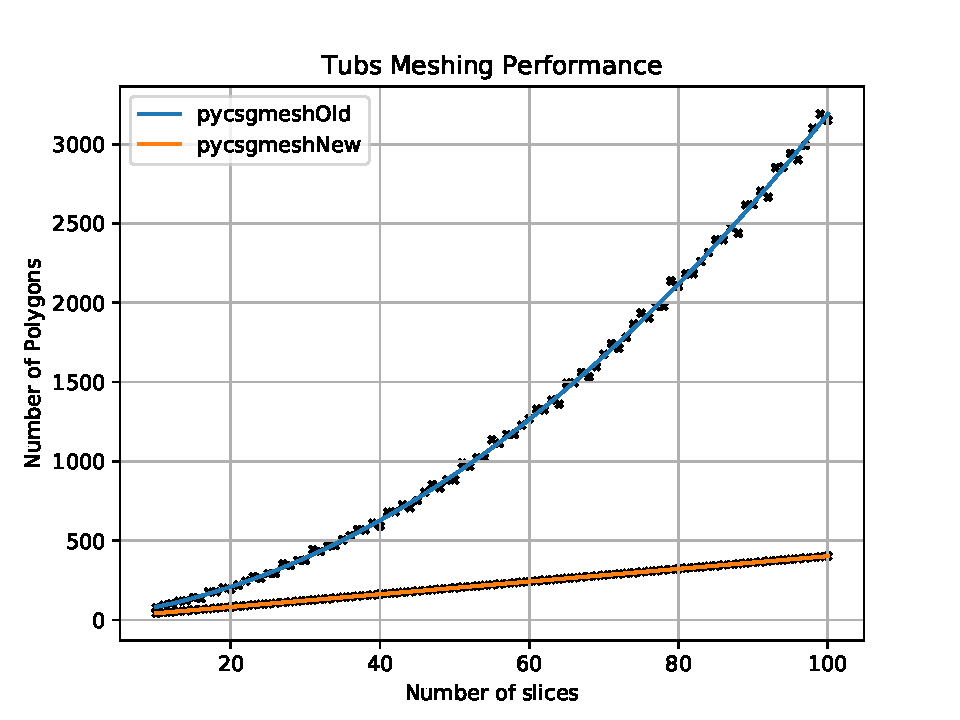
\includegraphics[scale=0.5]{Images//Quad_fits//Tubs_quad.pdf}
  \captionof{figure}{A plot showing the comparison of\\ the number of polygons (and triangles) generated\\ by the new and old meshing methods, across a\\ range of slices 10-100.}
  \label{conts}
\end{minipage}%
\begin{minipage}{.5\textwidth}
  \centering
  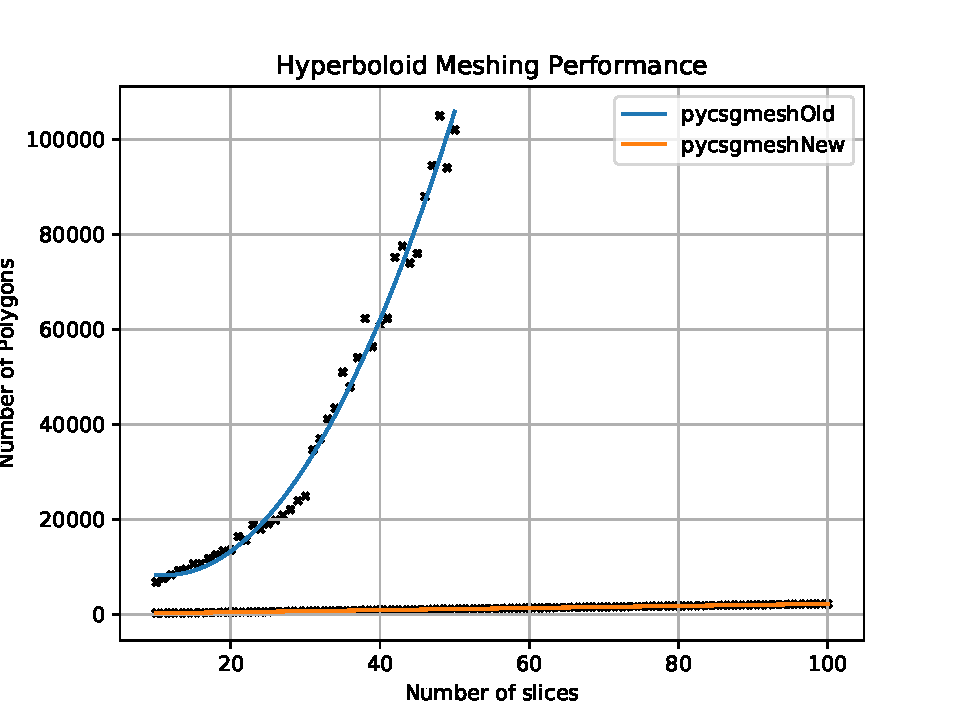
\includegraphics[scale=0.5]{Images//Quad_fits//Hyperboloid_quad.pdf}
  \captionof{figure}{A plot showing the comparison of\\ the number of polygons (and triangles) generated\\ by the new and old meshing methods, across a\\ range of slices 10-100.}
  \label{hypeup}
\end{minipage}%
\end{figure}

\newpage
\noindent Figures \ref{conts} \& \ref{hypeup} are two of many plots, which are all displayed in the Appendix \ref{app1}. As you can see in  both Figures, the new meshing function is much more computationally reduced compared with the old meshing functions, generating far less faces per slice and stack. The number of polygons increases more uniformly and linearly for the new pycsgmesh() function. On the hand the old pycsgmesh() function exhibits a more scattered and quadratic relationship, due to the boolean operations. This is also confirmed by the values tabled in the Appendix \ref{tab1}, which contains the quadratic fitting parameters to all the polygon count plots. If you extrapolated both graphs it is clear than the new mesh is not only improving the structural appearance of the meshed solids, but also saving large amounts of computational power and time.
\\\\
\label{recur}
\noindent The next section goes on the test spheres of varying slice and stack within BDSIM. Figure \ref{tritri} shows the total number of triangles on the interior and exterior surfaces for a given slice and stack equal to the same value on a G4\_Ti sphere. The old meshing would only meshed up to a maximum resolution of slice and stack equaling 48, before it would max out Pythons recursion limit. Where as the new meshing could go to 100 stack, 100 slice with out any issues at all. The recursion limit can be extended to allow for a larger range, however it would not be worth the time it would tke to code and run. As all it would prove is that the new code is still much faster. 

\begin{figure}[h!]
\centering
\begin{minipage}{.5\textwidth}
  \centering
  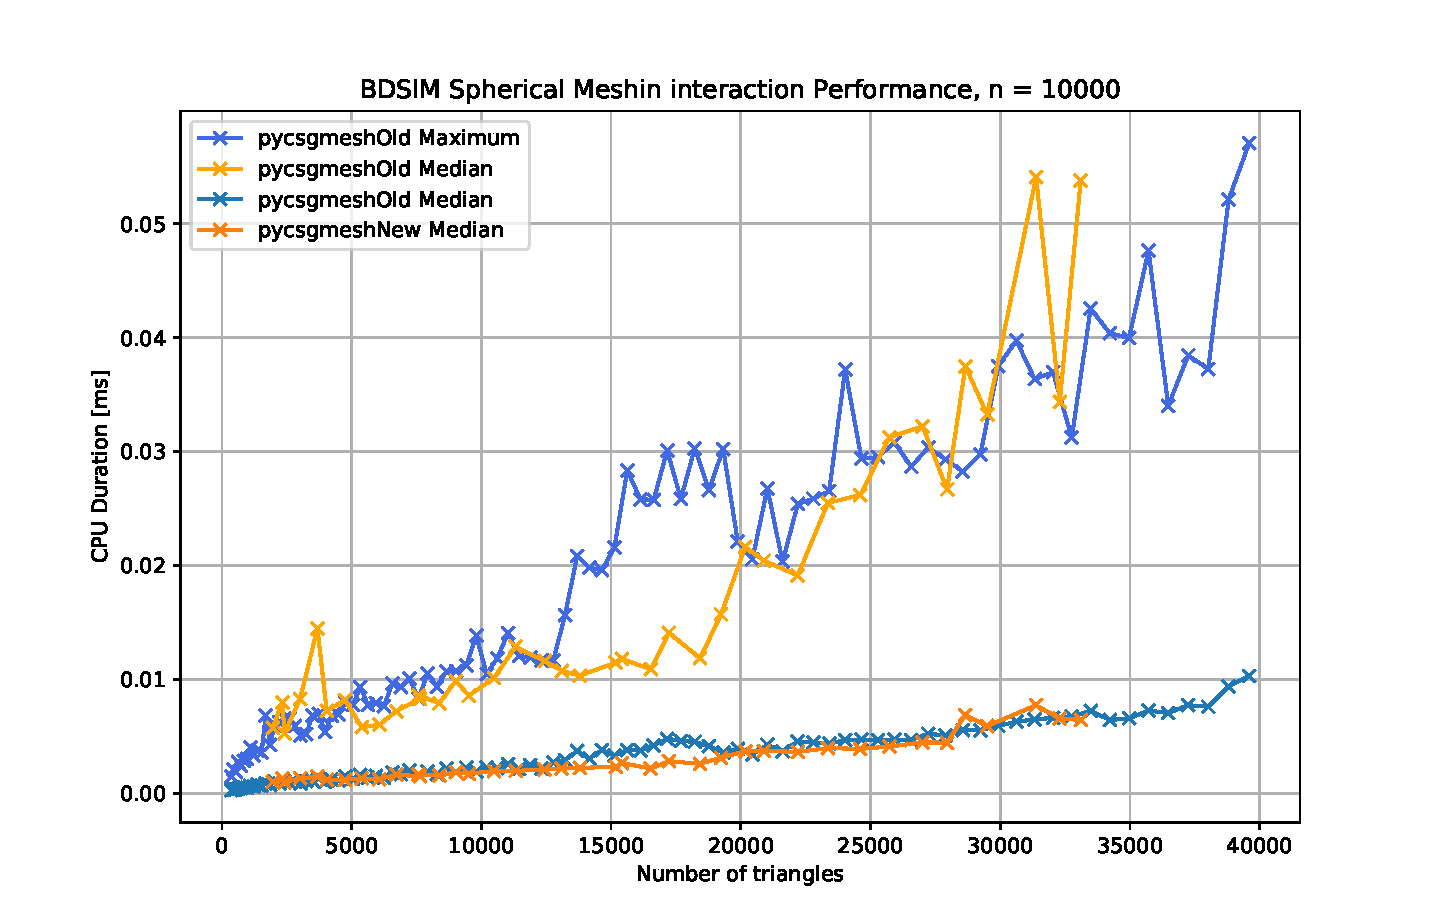
\includegraphics[height=0.7\linewidth]{Images//CPU//mednmax.pdf}
  \captionof{figure}{TODO}
  \label{mednmax}
\end{minipage}%
\begin{minipage}{.5\textwidth}
  \centering
  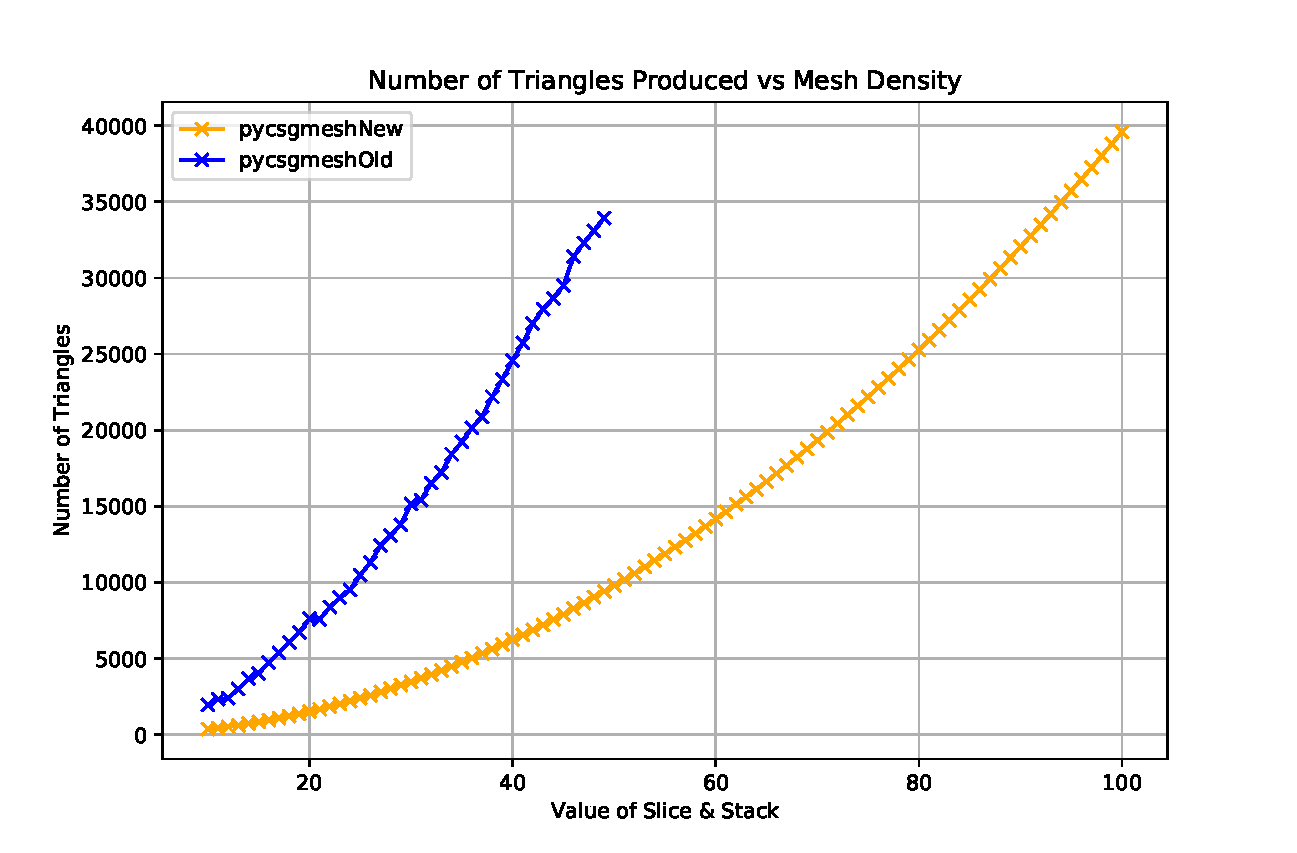
\includegraphics[height=0.7\linewidth]{Images//Triangles//MeshvTRi1.pdf}
  \captionof{figure}{TODO}
  \label{tritri}
\end{minipage}%
\end{figure}

\noindent It can be seen that in Figure \ref{tritri} the new pycsgmesh() function has a much smooth gradient and that the old function has small peaks occurring at certain intervals of stack and slice. This is most likely to do with the boolean subtractions of the spheres favouring the old mesh at particular densities

%---------------------------------------------------------------------------------------------------
%---------------------------------------------------------------------------------------------------
%---------------------------------------------------------------------------------------------------

\section{BDSIM Interactions}
\label{int}
The second aim of this project was to measure how the physics is altered, between the new and old meshings as the mesh density is varied. As mentioned before GEANT4 already has its own set of primitive solids, which can be used as a guideline for comparison, due to no slice and stack dependence. The physics being measured will be features such as the trajectories and energy deposition, through solids.

\begin{figure}[h!]
\centering
\includegraphics[scale=0.33]{Images//BDSIM//titanium.pdf}
\caption[width=\columnwidth]{A BDSIM screenshot of a G4\_W GEANT4 Sphere generated with new meshing interacting with 1.3 GeV electrons.}
\label{black}
\end{figure}

\noindent BDSIM uses the colour convention for representing a particles charge from GEANT4, green is neutral, blue is positive and red is negative. Figure \ref{black} shows a spherical distribution of 100 1.3 GeV electrons radiating outwards from the centre of a G4\_Ti sphere, where it can be seen that red electrons and many green neutron secondaries are produced. A secondary particle is anything that is produced as a result of the initial particles interacting with the solid, therefore a secondary itself can produce anther particle which is considered to also be  a secondary particle. The Monte Carlo simulation in BDSIM uses a numbering system for storing particles, assigning each particle a unique number for ease of identifying what happens in a set interaction. The numbering system adopted in BDSIM is the one created by PDG (or the Particle Data Group) \cite{pdg}, which is an international collaboration dedicated to analysing and publishing the properties of particles. 

\subsection{Monte Carlo Simulation}
\label{monte}
\noindent The probability of certain particle interactions occurring in a given BDSIM event, such as the decays or scattering of a particles trajectories is generated by a Monte Carlo simulation.The basic principle behind the Monte Carlo algorithms is the use of large random sampling to find numerical results. This is perfect for simulating the probabilities of particular particle interactions happening, as two initially identical interaction setups can have two non identical interactions, with a given probability. Each event in BDSIM is associated with a specific seed number produced via this Monte Carlo method. The uniqueness of each seed allows a particular event to be repeatedly simulated under the same physics conditions, which is key to this project when it comes to comparing the interactions of different objects fairly. The other properties of the particle and physics processes that may occur can also be user defined to tweak the experiment. Properties such as the particles initial energy, whether secondaries get produced and much more. The seeds used in this project could not be logically chosen due to the fact they are generated via the Monte Carlo simulation. Therefore they were selected by running a lot of test runs in BDSIM to see which seeds generate a decent amount of secondaries.

\subsection{Simulation Execution}
BDSIM works by running a GMAD file and then outputs  a ROOT (Section \ref{root}) file with the option of using the GUI, allows the user to visualise the interactions in an interactive 3D environment. A GMAD file contains the basic information needed to produce an interaction in BDSIM, i.e a particle and path to file of the target object (Typically of the format GDML). The option ``physicsList'' defines the physics which is used for the interaction, for the project the option was set to``g4FTFP\_BERT'', which contains all the standard electromagnetism and particle physics required for this project. The ROOT file contains a detailed analysis of the interaction. One of the elements analysed within this project is the CPU duration time distribution of an interaction in BDSIM.

\newpage
\subsection{Sampling}
The meshed solid chosen to be tested within BDSIM for this project was the sphere, which is made of a minimum and maximum radius, making it a hollow solid. The reason a sphere was chosen because it is the ideal shape testing radiation in all directions, as its thickness can be controlled radially. As seen in Figure \ref{sphbd} the sphere was orginally chosen to be oriented such that the particle beam is fired from the centre of the sphere outwards. The conversion from a Pyg4ometry mesh into a GEANT4 tessellated solid, results in only triangular faces. This is why all the quadrilateral faces are cut into two in Figure \ref{sphbd}.

\begin{figure}[h!]
\centering
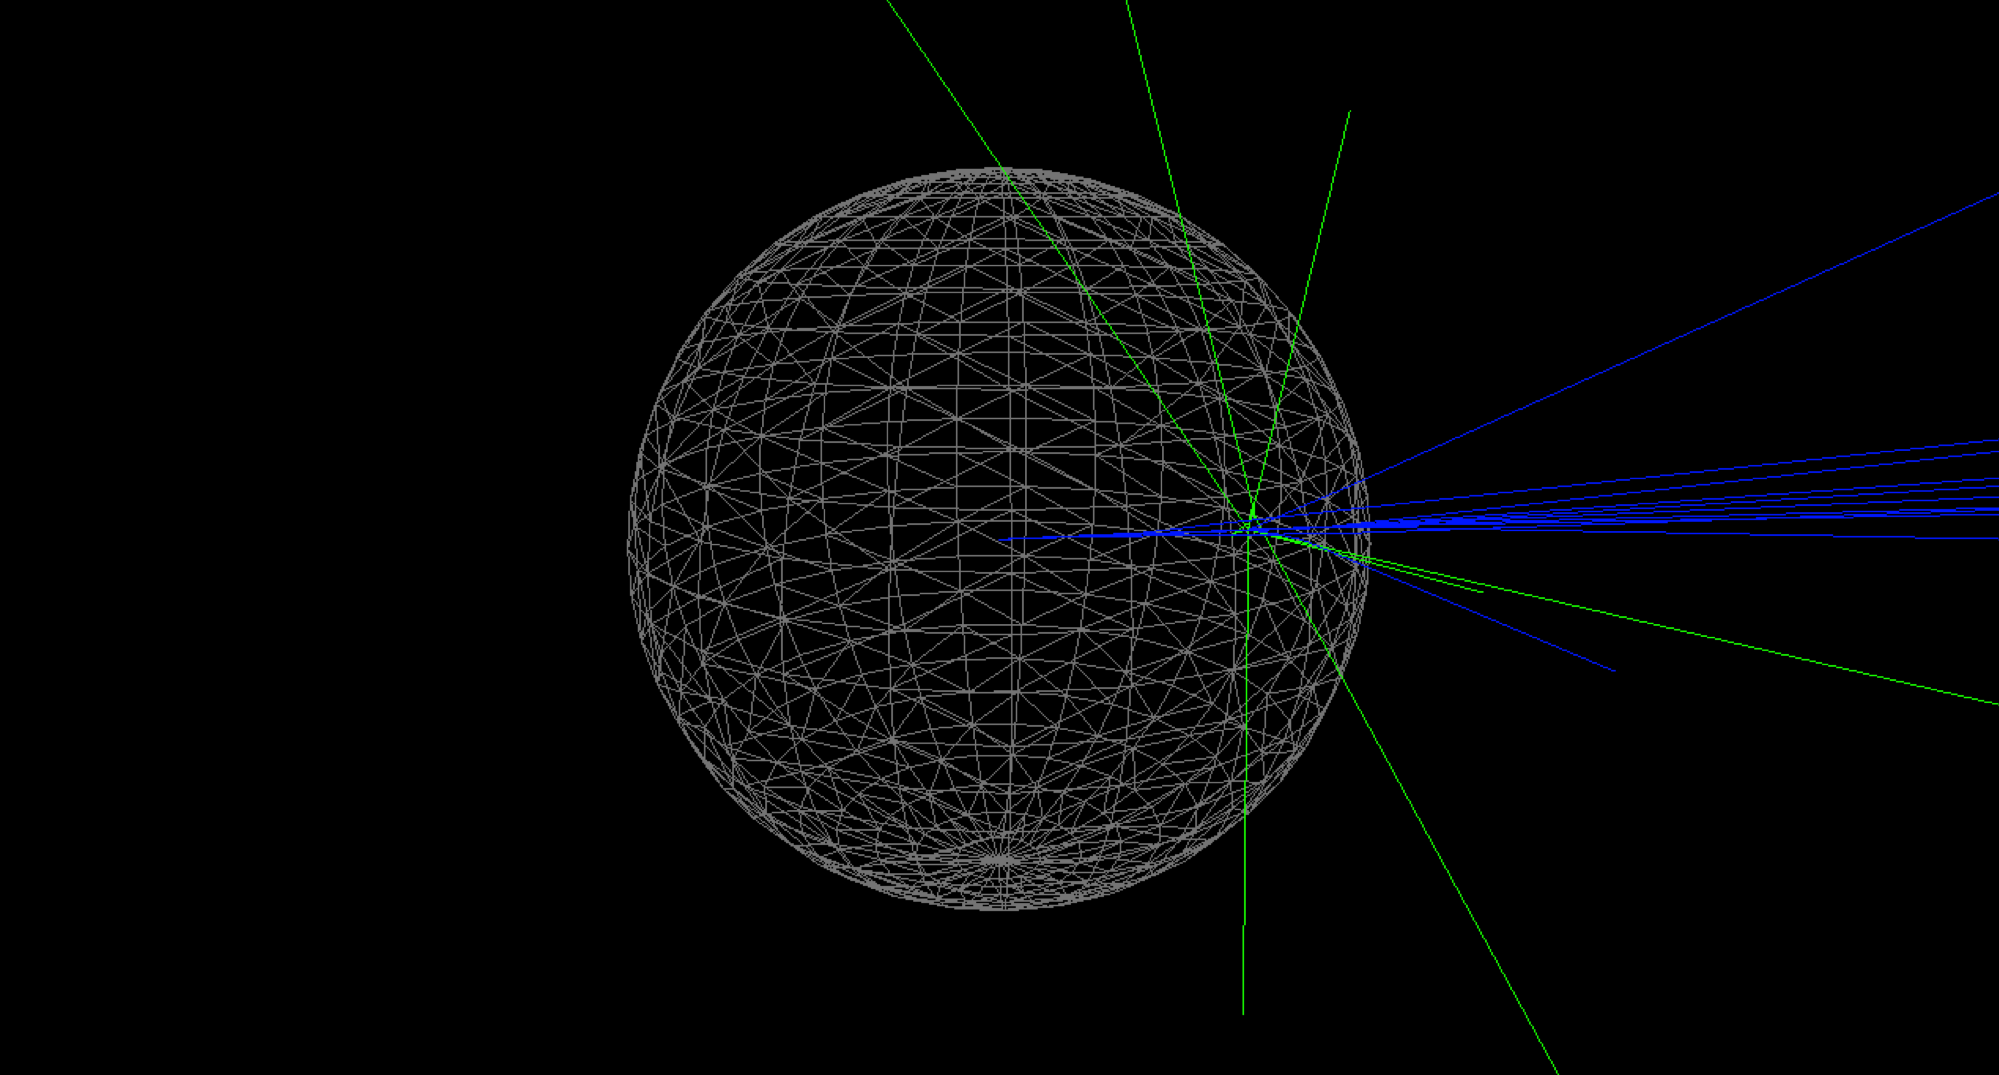
\includegraphics[scale=0.35]{Images//BDSIM//ProtonSphere2.png}
\caption[width=\columnwidth]{BDSIM screenshot of 10 1.3 GeV protons interacting with a Iron sphere, which has been constructed using the new meshing scripts. Mesh resolution is a stack \& slice of 25 \& 25. (Shown in mesh view)}
\label{sphbd}
\end{figure}


\noindent One way that was though to analyse the energy deposition of the interactions, was to look at the CPU duration times as the mesh densities are increased. In this scenario the GEANT4 solid was used as a guideline as it does not depend on a user defined stack \& slice. 


\subsection{Titanium Sphere Interactions}

In this section the CPU duration time of interaction in BDSIM with spheres of different mesh densities by different meshing algorithms. Table \ref{tab1} shows the properties of the spheres being meshed.
 
\begin{table}[h!]
\centering
\begin{tabular}{|l|l|}
\hline
Property & value \\ \hline
$R_{Min}$ &  8.00 [mm]\\ \hline
$R_{Max}$ &  10.00 [mm]\\ \hline
Particle &  $e^-$\\ \hline
Energy & 1.3 GeV [MeV]\\ \hline
ngenerate & 10,000\\ \hline
\end{tabular}
\caption{Table of sphere properties for the simulations in this section}
\label{tab1}
\end{table}

\noindent Figure \ref{withs} shows the mean CPU duration times for an interaction in BDSIM with a given sphere. The x-axis was orginally the number of stack and slice, but it was thought that the number of triangular created for a given sphere would give a fairer weighting. The reason there is nearly twice as many points plotted for the new meshing over the old is because of the recursion limit, which is discussed in Section \ref{recur}. The error bars in Figure \ref{withs} is the std deviation of each run, the material of the sphere was orginally chosen to be G4\_Fe which is much less dense and causes many more secondaries that G4\_Ti, making the error bars to big to clearly read the data trend. The second plot on the left Figure \ref{withs} is the same simulation as in figure \ref{withs}, but has secondary particles disabled. The reason for Figure \ref{withouts} is to show that the number of secondaries produced has an effect on the duration of the interaction.
\\\\
\begin{figure}[h!]
\centering
\begin{minipage}{.5\textwidth}
  \centering
  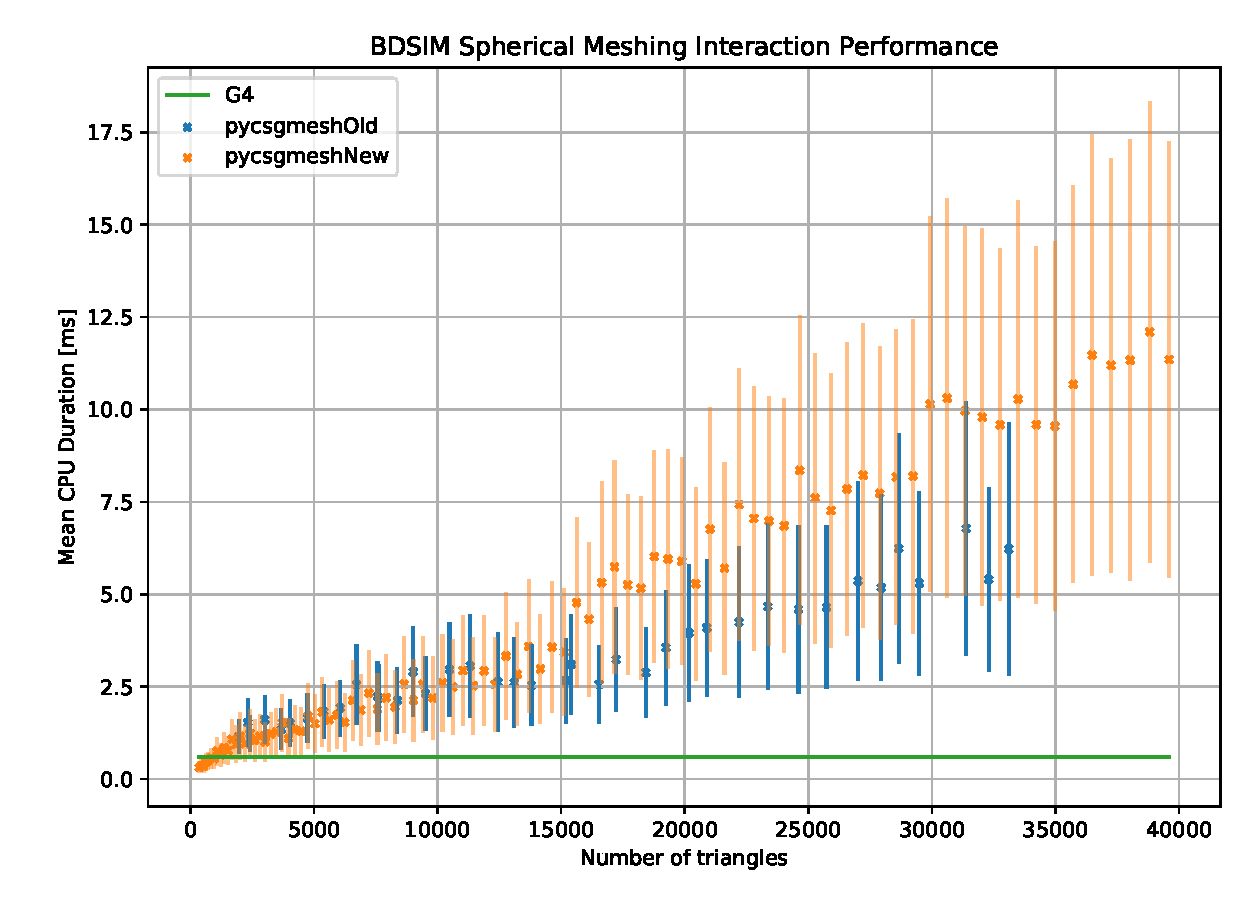
\includegraphics[height=0.7\linewidth]{Images//CPU//Total_Plot_with_secondaries.pdf}
  \captionof{figure}{A plot showing mean CPU\\ duration of 10,000 protons interacting with a\\ Iron sphere of various meshed forms.\\}
  \label{withs}
\end{minipage}%
\begin{minipage}{.5\textwidth}
  \centering
  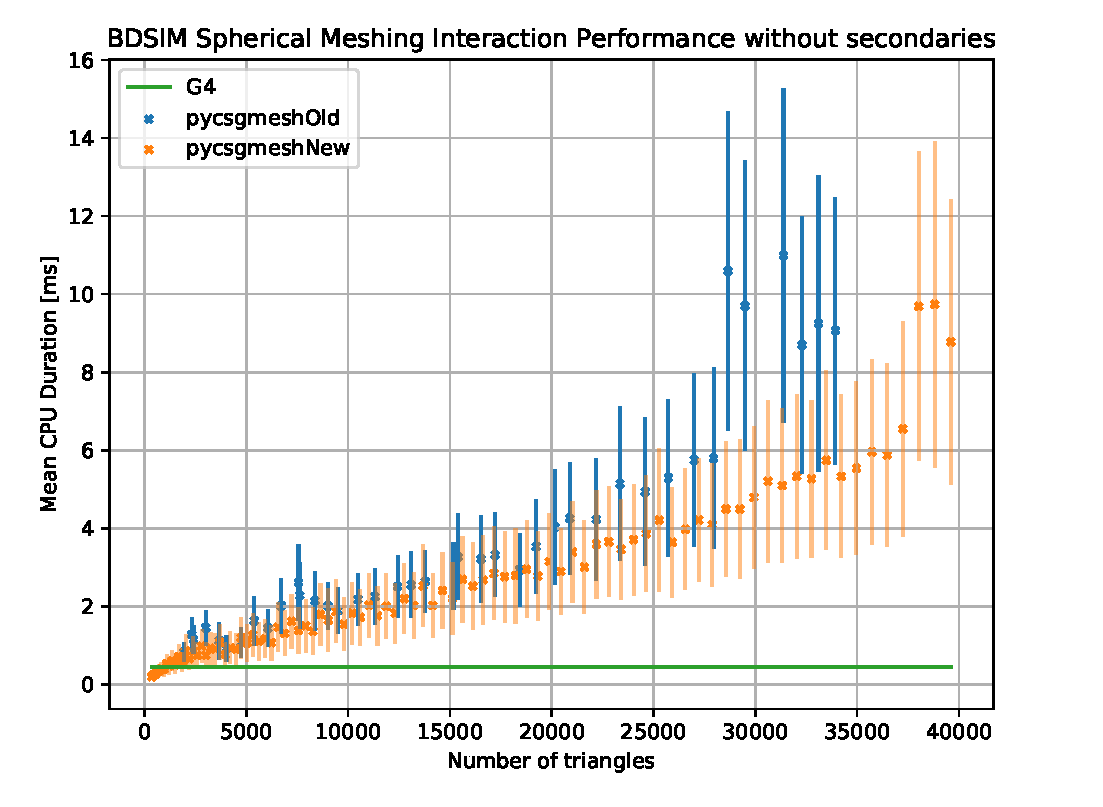
\includegraphics[height=0.7\linewidth]{{Images//CPU//Total_Plot_no_secondaries1.pdf}}
  \captionof{figure}{A plot showing mean CPU\\ duration of 10,000 protons interacting with\\ a sphere of various meshed forms, with secondary\\ particles disabled.}
  \label{withouts}
\end{minipage}%
\end{figure}

%\begin{figure}[h!]
%\centering
%\begin{minipage}{.5\textwidth}
%  \centering
%  \includegraphics[height=0.75\linewidth]{Images//CPU//Total_plot_with_offset.pdf}
%  \captionof{figure}{A plot showing mean\\ CPU duration of 10,000 protons\\ interacting with a Iron sphere of\\ various meshed forms, with\\ an 20 mm of set in the Z-axis.}
%  \label{cons}
%\end{minipage}%
%\begin{minipage}{.5\textwidth}
%  \centering
%  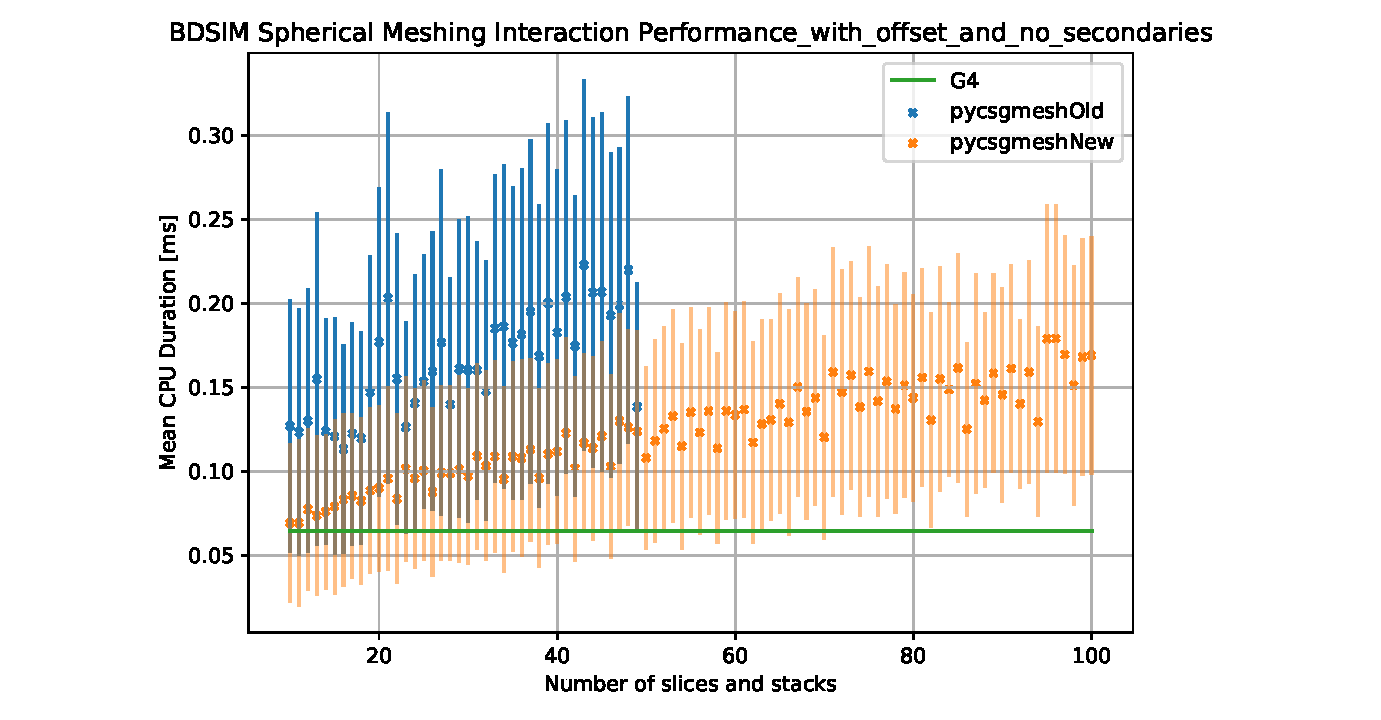
\includegraphics[height=0.75\linewidth]{Images//CPU//Total_Plot_with_offset_and_no_secondaries.pdf}
%  \captionof{figure}{ A plot showing mean\\ CPU duration of 10,000 protons\\ interacting with a Iron sphere of\\ various meshed forms, with\\ secondary particles disabled, with\\ an 20 mm of set in the Z-axis and secondaries disabled.}
%  \label{fig:test2}
%\end{minipage}%
%\end{figure}

\begin{figure}[h!]
\centering
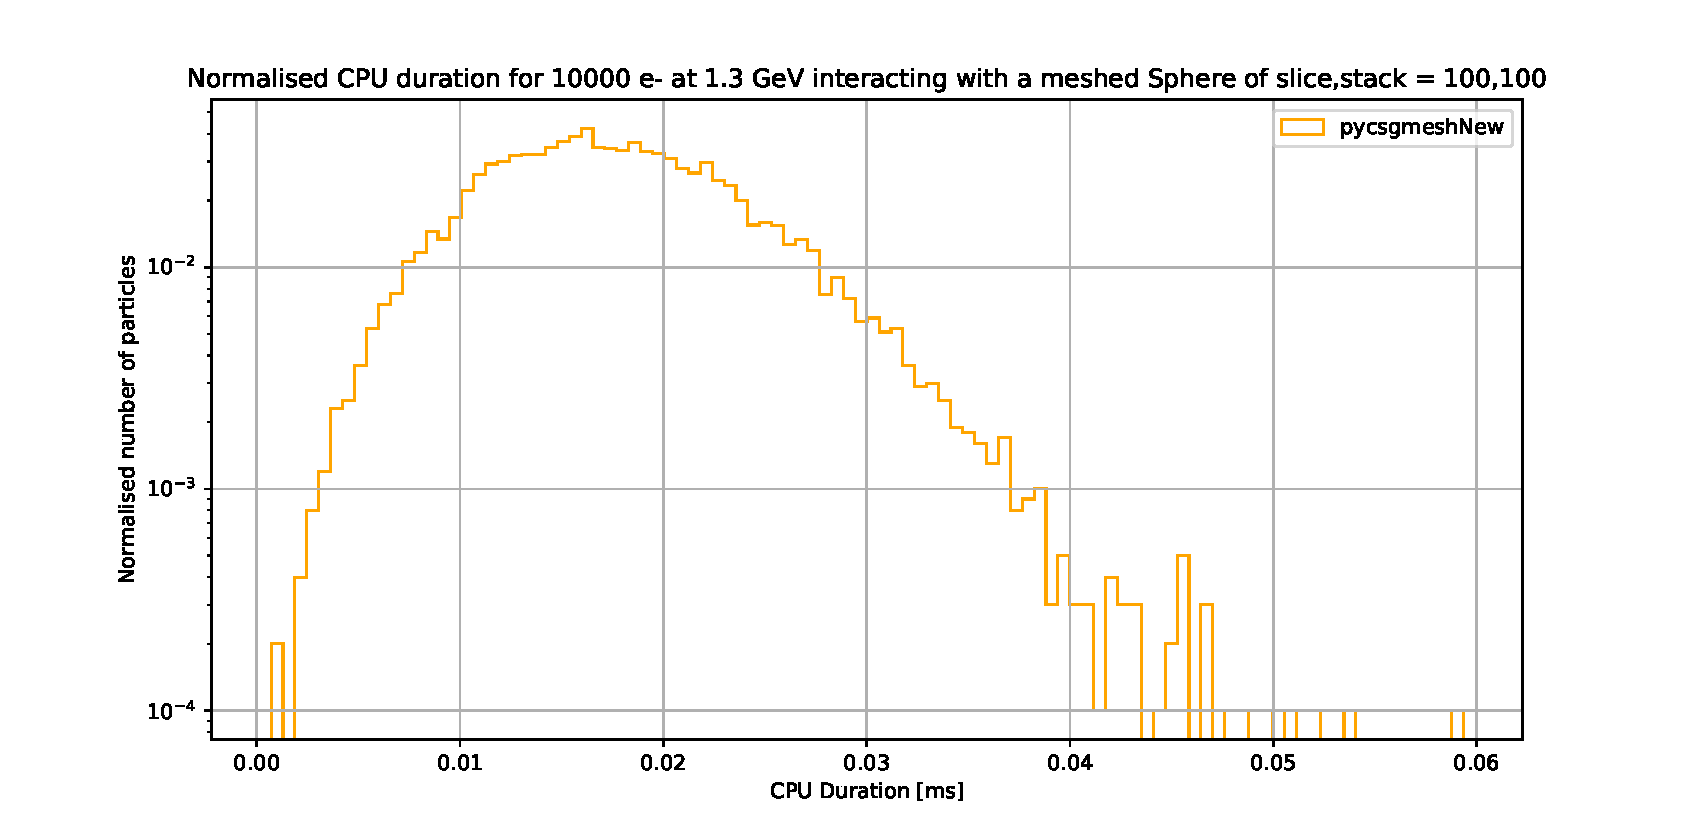
\includegraphics[scale=0.5]{Images//CPU//pythonhist1.pdf}
\caption[width=\columnwidth]{TODO}
\label{disty}
\end{figure}

\noindent The reason for the standard deviations being so large is to do with a small number of particles in each event having a longer lifetime, thus skewing the standard deviation of the whole event. An example of this is shown in Figure \ref{disty}, where the plot shows the CPU distribution for 10,000 10 MeV electrons interacting with a G4\_Au sphere. The sphere in this example is constructed using the new pycsgmesh() function with a stack and slice both set at 100.

\noindent From Figures \ref{} and \ref{}, you can see that as the number of stack and slice is increased the mean CPU duration for the protons increases at a slower rate for the new meshing. 
\\\
\noindent It was orginally thought that the standard deviations of the CPU durations was related to the number of secondaries being produced. However this was disproved by Figure \ref{}, where the same test was conducted with the BDSIM option that disables secondary particles from being produced implemented.

\subsubsection{Error Reduction}
To reduce the standard deviation of a data set the number of events needs to be increased, this proved by the relation ship shown in Equations \ref{std}. The relationship between the standard deviation and number of events is inversely square root proportional. Therefore the standard deviation should decrease with a increasing N.

\begin{equation}
\begin{aligned}
& \bar{x} = \frac{1}{N}\sum{x_i}\\
& \sigma = \sqrt{\bar{x}^2} = \sqrt{\frac{1}{N}\sum{(x_i - \bar{x}})^2}\\
& \sigma \propto \frac{1}{\sqrt{N}} 
\end{aligned}
\label{std}
\end{equation}

However Figure \ref{} shows...\\
\begin{figure}[h!]
\centering
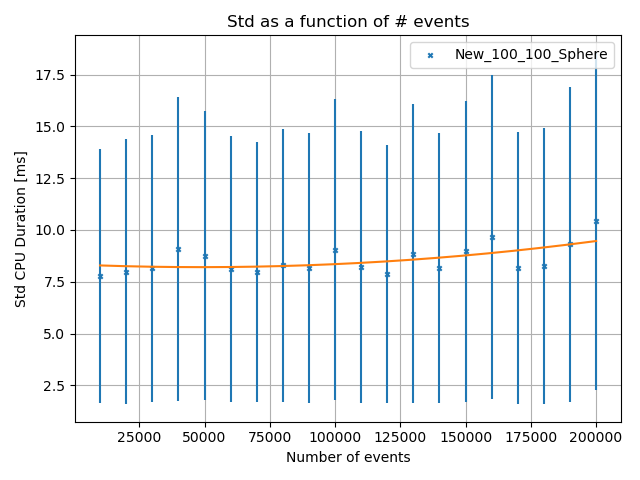
\includegraphics[scale=0.5]{Images//Error//std_N.png}
\caption[width=\columnwidth]{TODO}
\label{sphbd}
\end{figure}

The error bars are still very big so it was proposed to use the standard error of the main as an alternative. As well as as investigation for varying energy and the material of the target.

\subsection{Selection of Material}
When creating meshed solids, you have the choice of material. Figure \ref{novar} shows the CPU duration time distributions for electrons interactions with GEANT4 spheres constructed of different GEANT4 materials across a range of energies in BDSIM. The energy range is relatively low (25 MeV $\rightarrow$ 100 MeV), this is due to the run time of the interactions increasing with energy. The run time is heavily linked to the number of secondary particles which is a function of energy. This is proven by the fact that it can be seen that as the energy is increased the width of the distribution increases. This widening is due to the number of secondary particles being produced, the more energetic an interaction the further the particle will penetrate a solid and ionise along the way generating more secondaries.

\begin{figure}[h!]
\centering
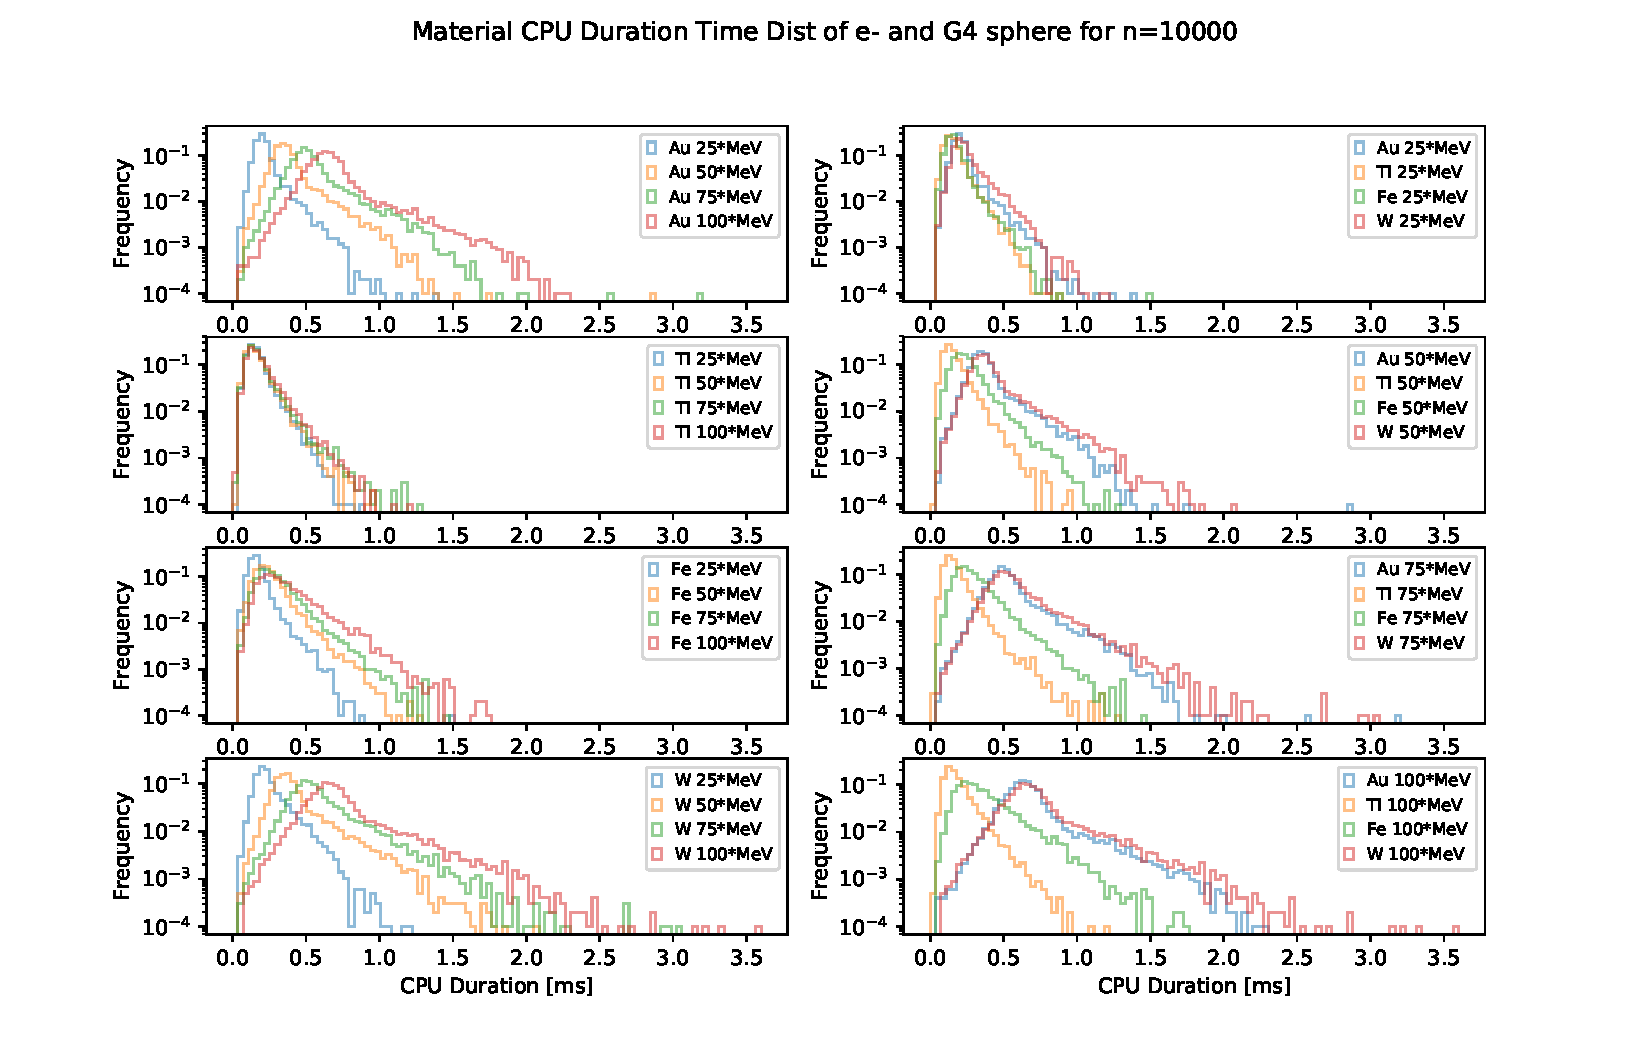
\includegraphics[scale=0.6]{Images//Materials//not_Varied_by_radius_and_secondaries.pdf}
\caption[width=\columnwidth]{Histograms showing the CPU duration distributions of varying GEANT4 materials and particle energies in BDSIM on a GEANT4 sphere. The left 4 histograms show the distributions show the varying of energy upon each material. The right 4 histograms show the varying of material at each set energy. Each plot is normalised by the initial 10,000 electrons in each event.}
\label{novar}
\end{figure}

\noindent The dimensions of the spheres used in Figure \ref{novar} were set to a minimum radius of 1 micron and a maximum radius of 20 mm. It was then proposed that the radius of thickness could be scaled with respect to the stopping distance of the material it is travelling through, in order to eliminate material as a variable. The radius of thickness $\Delta R$ can be seen depicted in Figure \ref{deltar}, where $\Delta R = R_{Max} - R_{Min}$. The next Section discusses the stopping power of materials in more detail.

\begin{figure}[h!]
\centering
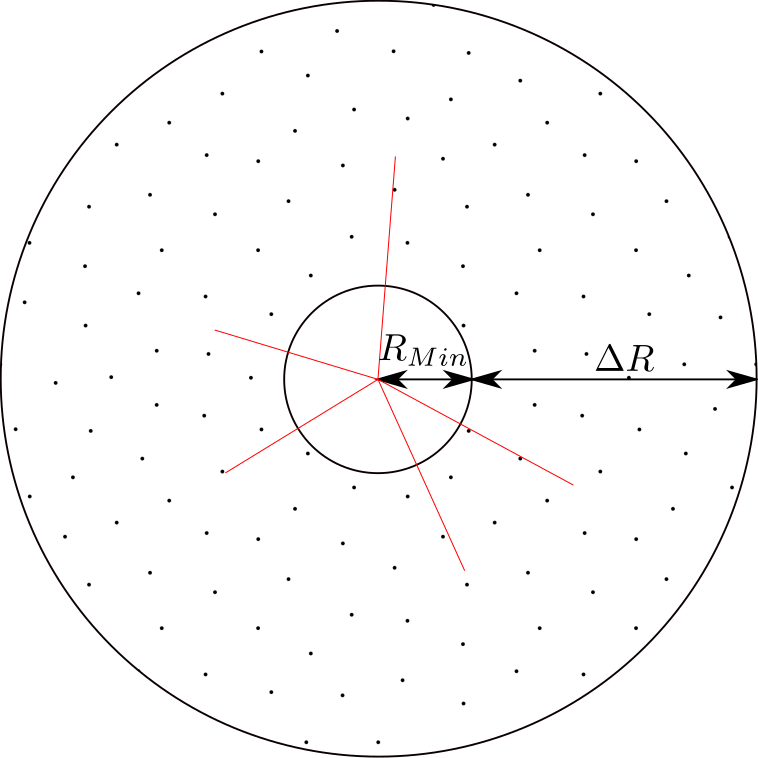
\includegraphics[scale=0.2]{Images//Materials//RMAX.png}
\caption[width=\columnwidth]{A diagram depicting a cross section of a sphere, which has a minimum and maximum radius. The diagram was drawn using the CAD software Inkscape.}
\label{deltar}
\end{figure}

\newpage
\subsubsection{Stopping Power}
\label{stop}
Stopping power is the force that acts against the motion of a particle within in a material, causing it to lose energy. A charged particle is mainly slowed down by electronic stopping as it moves along a linear trajectory. Electronic stopping is the inelastic energy loss to the electrons of the target as a result of thermal vibrations at an atomic level. The electronic stopping contributes most in the intermediate energy range of a travelling particle, as seen in Figure \ref{stprg}. Once the particle has lost a sufficient amount of its energy, slowing its velocity through the target, the probability of an elastic collision with a nuclei increases (Nuclear Stopping). The nuclear stopping is the process which causes damage to the target, as the target atom recoils way after the interaction causing a disorder in the lattice structure of the target. The recoiled atom can also go on to cause further collisions causing yet more damage. AS seen in Figure \ref{stprg} the electronic stopping power dominates and the nuclear stopping only needs to be accounted for at low energies.
\\\\
\begin{figure}[h!]
\centering
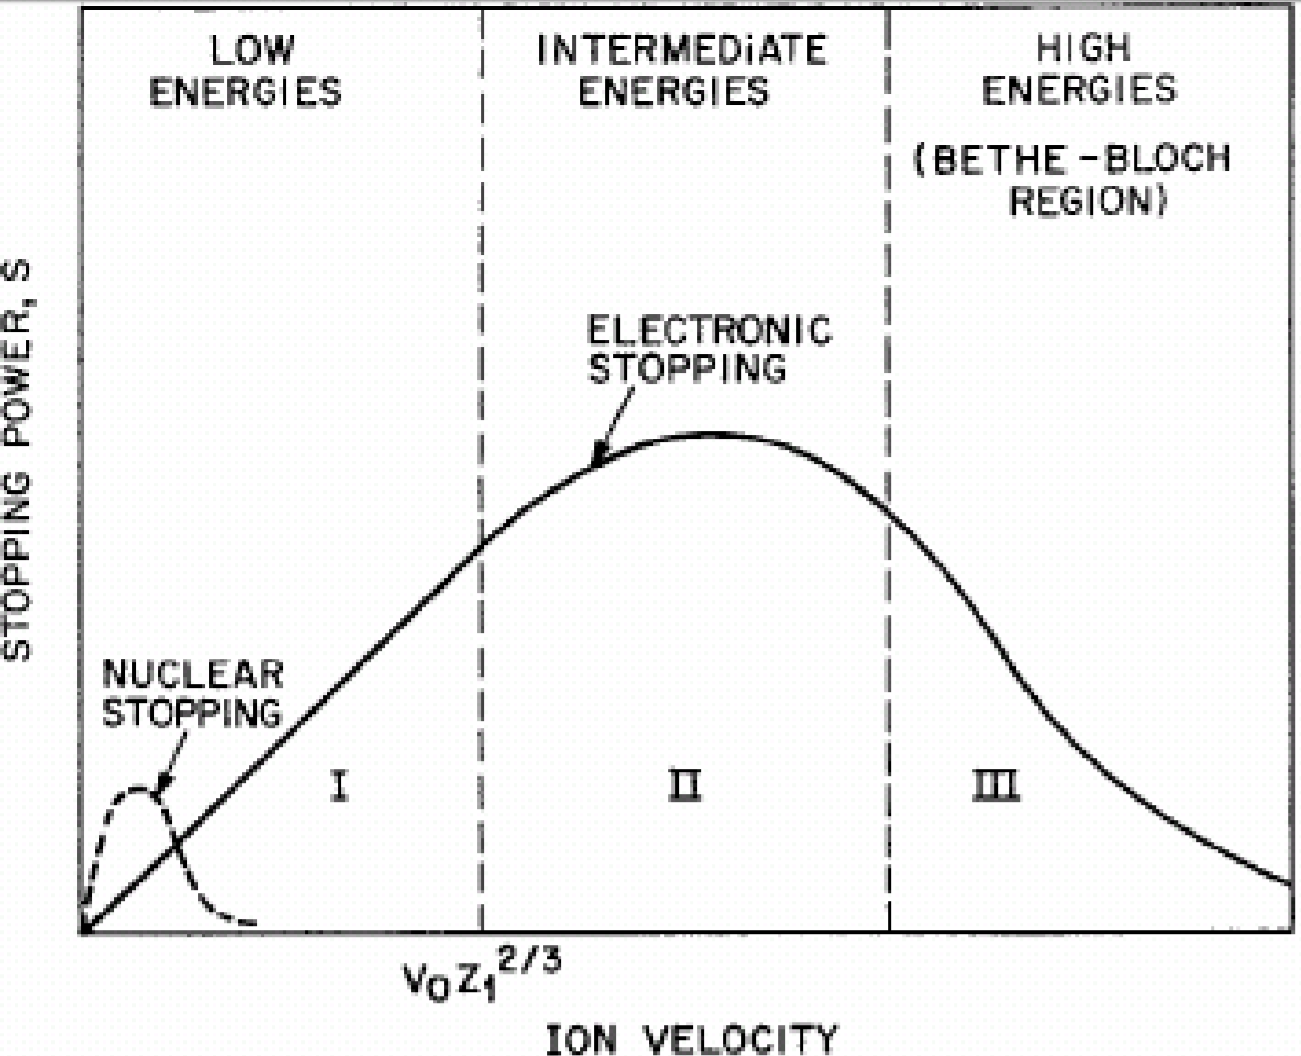
\includegraphics[scale=0.4]{Images//Stopping//stoppingrange.png}
\caption[width=\columnwidth]{A plot showing the relationship between ion velocity and components of stopping power. Figure 2.1 from Source \cite{stprg}}
\label{stprg}
\end{figure}
\\\\
\noindent The GEANT4 example ``TestEm0'' \cite{emo} outputs the stopping power and distances for a given material and particle energy. If the energy of the incident particle and the stopping power of the material is known, a stopping distance can be calculated. The values for stopping power in this project are calculated by the TestEm0 example, which extracting values from a GEANT4 data lists and then interpolates or extrapolates between them, as the stopping power is a function of. The extracted stopping powers match with values found in other studies, such as \cite{stpdat}.
\\\\
Figure \ref{tung} shows a sphere made of G4\_W, undergoing interactions with batches of 100 electrons at 3 different energies. The spheres radius of thickness is set to the be the stopping distance for G4\_W interacting with a 1 TeV electron. It can be seen that when the energy of the electrons is 1 GeV, which is below the 1 TeV (the stopping distance energy for this situation), the tracks of the interactions are al contained within the sphere. The opposite happens when the electrons energies are more than 1 TeV, where most if not all of the particle tracks leave the sphere. 

\begin{figure}[h!]
\hspace*{1.4cm}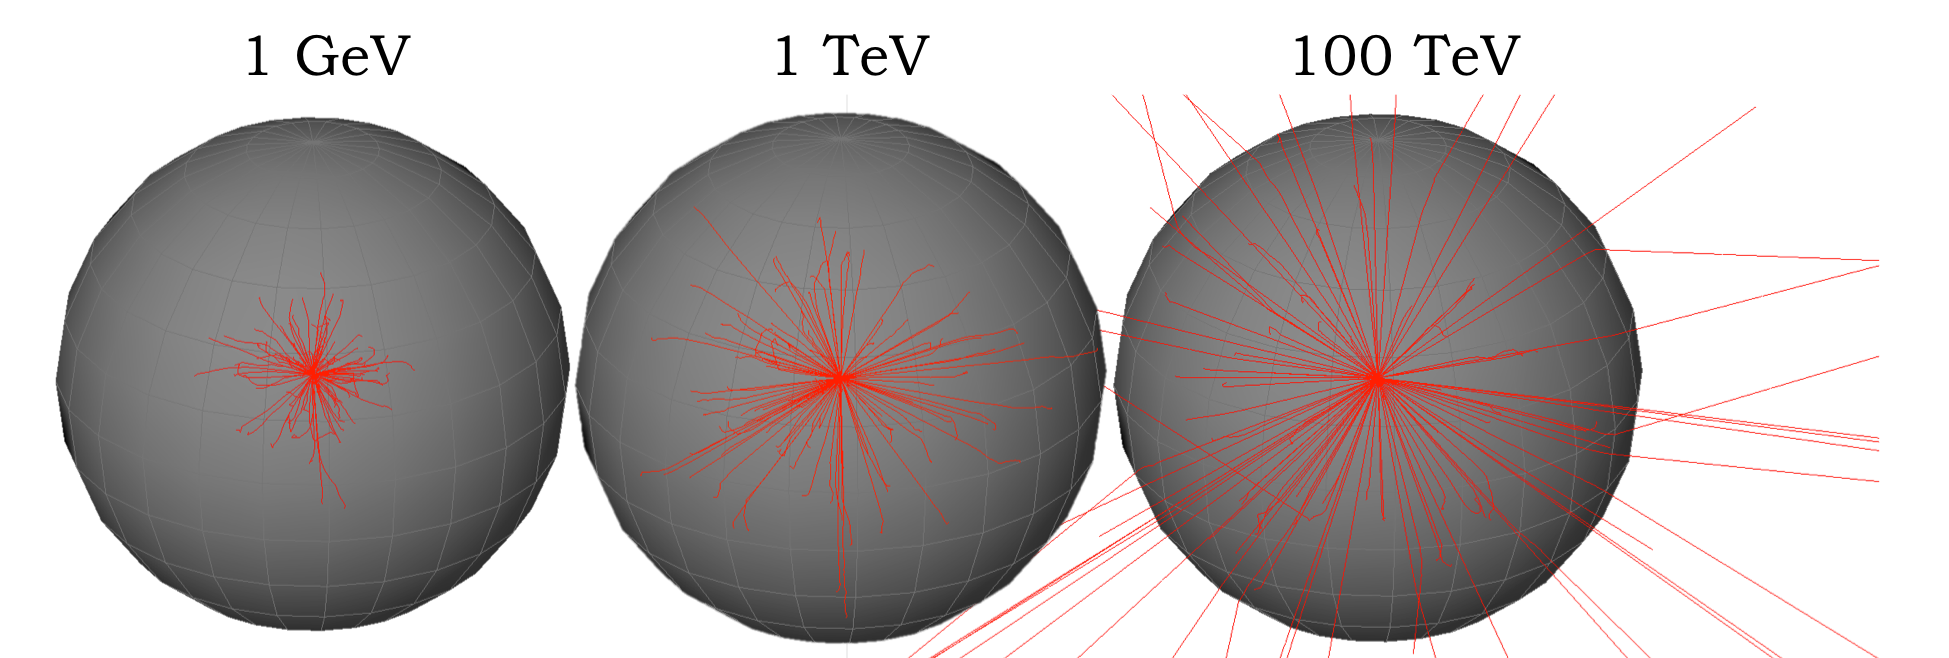
\includegraphics[scale=0.5]{Images//BDSIM//Tungsten_Sphere.png}
\caption[width=\columnwidth]{Screenshots of 1 GeV, 1 TeV \& 100 TeV electrons interacting with a tungsten sphere. Where the radius of thickness is set to the extracted GEANT4 stopping distance of a 1 TeV electron in tungsten.}
\label{tung}
\end{figure}

\noindent With the stopping power in mind Figure \ref{novar} was reproduced, but instead of using the same dimensions for each sphere, $\Delta R$ was scaled by the stopping distance. The radius of thickness is set to be the extracted stopping distance for a 100 MeV electron interacting with the material in question. The values of $\Delta R$ are shown in Table \ref{rs}.

\begin{table}[h!]
\centering
\begin{tabular}{|l|l|}
\hline
Material & $\Delta R$ [mm] \\ \hline
G4\_Au &  9.89382\\ \hline
G4\_Ti &  33.6854\\ \hline
G4\_Fe &  62.3434\\ \hline
G4\_W &  10.1631\\ \hline
\end{tabular}
\caption{A table showing the values of $\Delta R$ used in Figure \ref{var}.}
\label{rs}
\end{table}

\begin{figure}[h!]
\centering
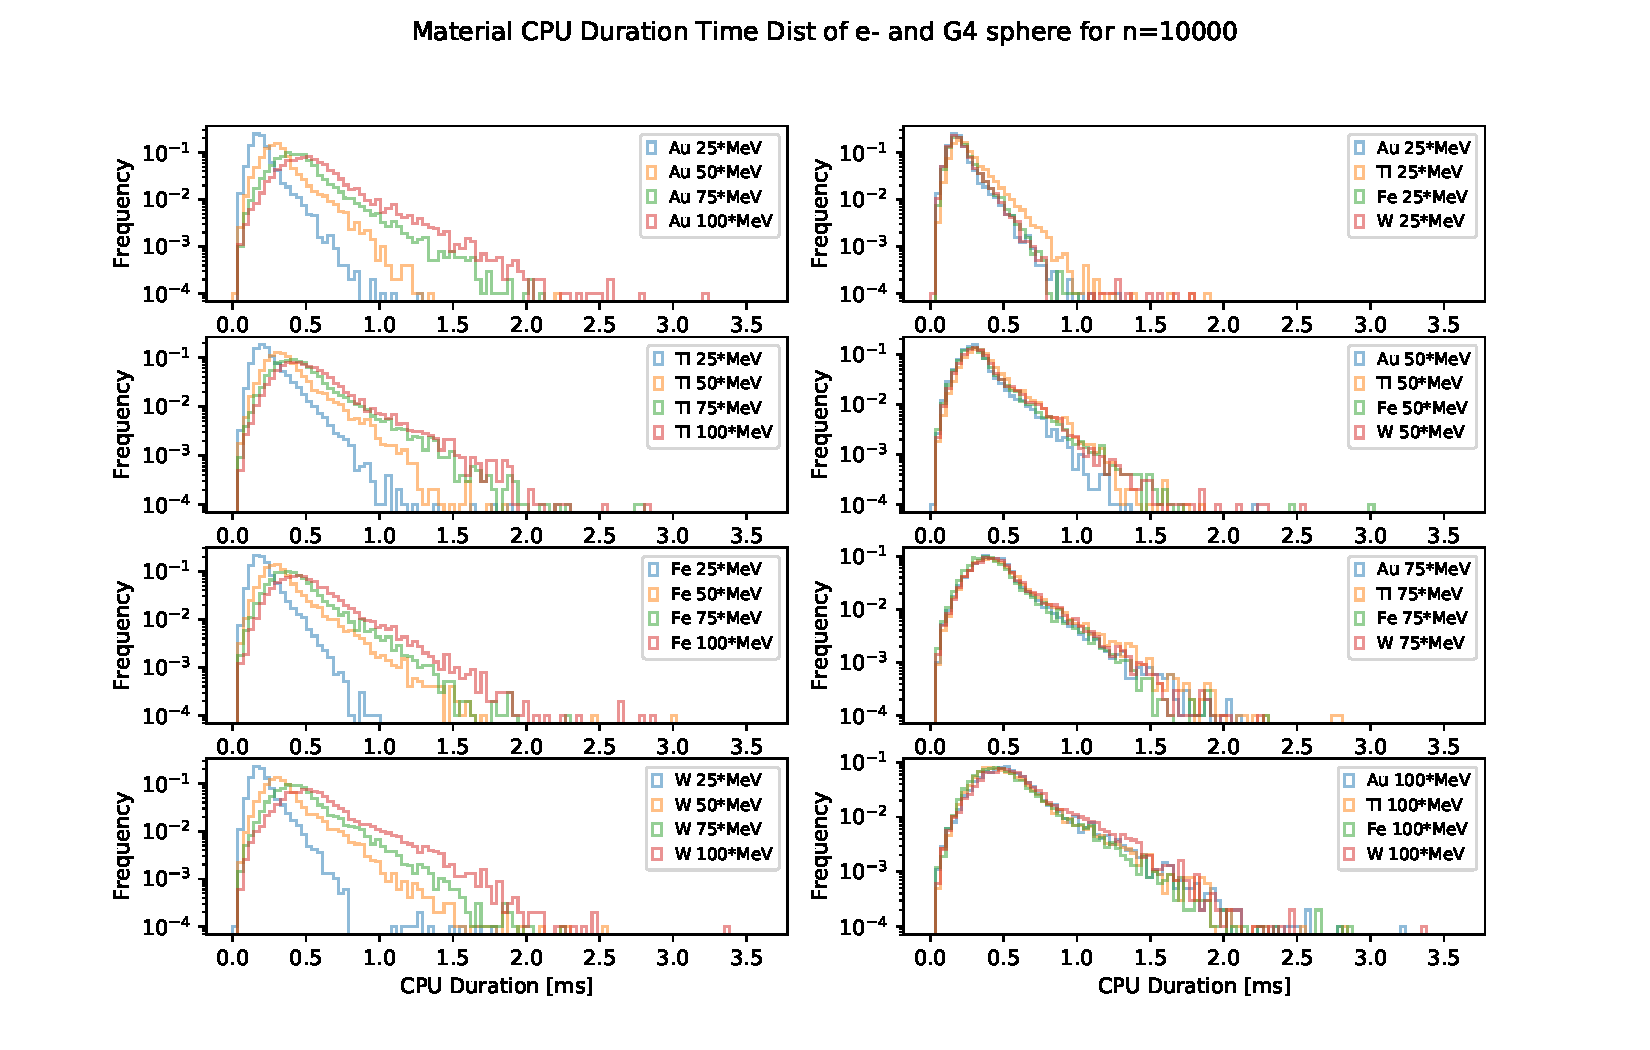
\includegraphics[scale=0.6]{Images//Materials//Varied_by_radius_and_secondaries.pdf}
\caption[width=\columnwidth]{Histograms showing the CPU duration distributions of varying materials and particle energies in BDSIM on a GEANT4 sphere. The left 4 histograms show the distributions show the varying of energy on each material. The right 4 histograms show the varying of material at a set energy. Each plot is normalised by the initial 10,000 electrons in each event.}
\label{var}
\end{figure}

\noindent It can be seen that in Figure \ref{var}, the scaling of radius relative to stopping distances, generates histograms which act extremely similar at the same particle energies irrespective of the material it propagates through. This is very interesting as it means that for any further analysis, material can be ruled out as a variable and only energy needs to be varied.

\begin{figure}[h!]
\centering
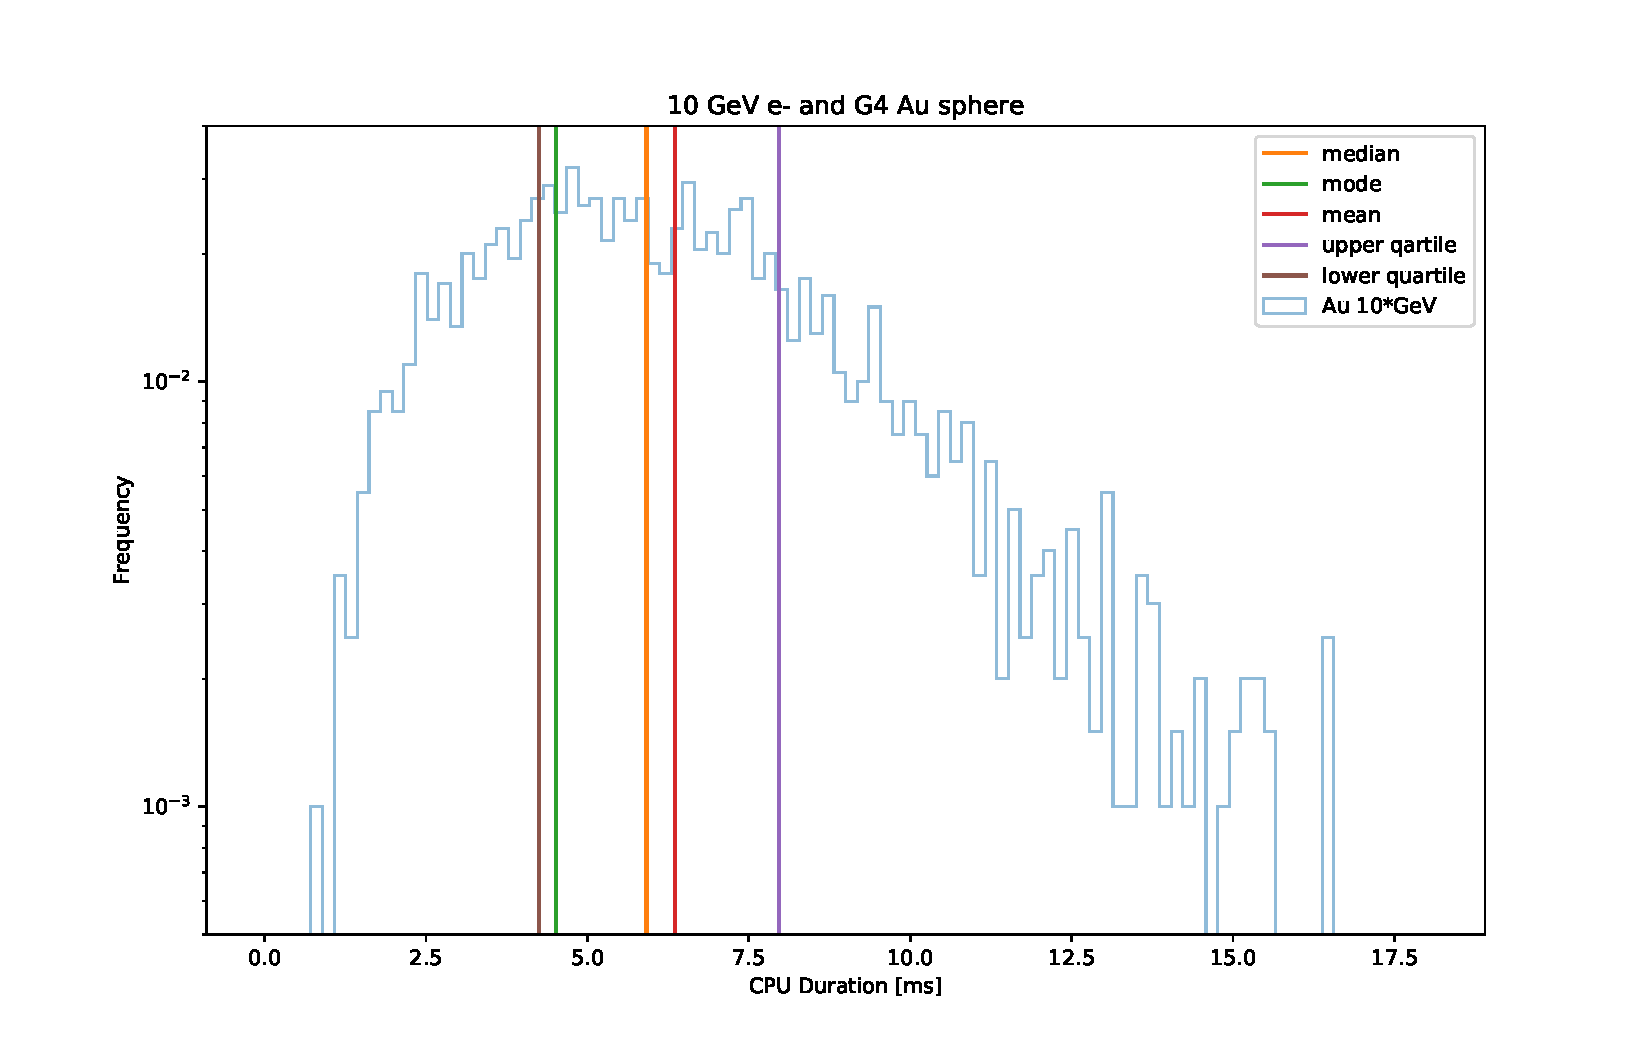
\includegraphics[scale=0.4]{Images//Materials//Time_ex_dists.pdf}
\caption[width=\columnwidth]{Meshing Development for Tubs (Solid \& Mesh View)}
\label{tubspic}
\end{figure}

%\newpage
%\subsection{Titanium Sphere Interactions \& Spherical Beam Distribution}
%
%\begin{table}[h!]
%\centering
%\begin{tabular}{|l|l|}
%\hline
%Property & value \\ \hline
%$R_{Min}$ &  0.01 [mm]\\ \hline
%$R_{Max}$ &  10.00 [mm]\\ \hline
%Particle &  $e^-$\\ \hline
%Energy & 10 [GeV]\\ \hline
%ngenerate & ?\\ \hline
%\end{tabular}
%\caption{TODO}
%\label{rs}
%\end{table}
%
%\begin{figure}[h!]
%\centering
%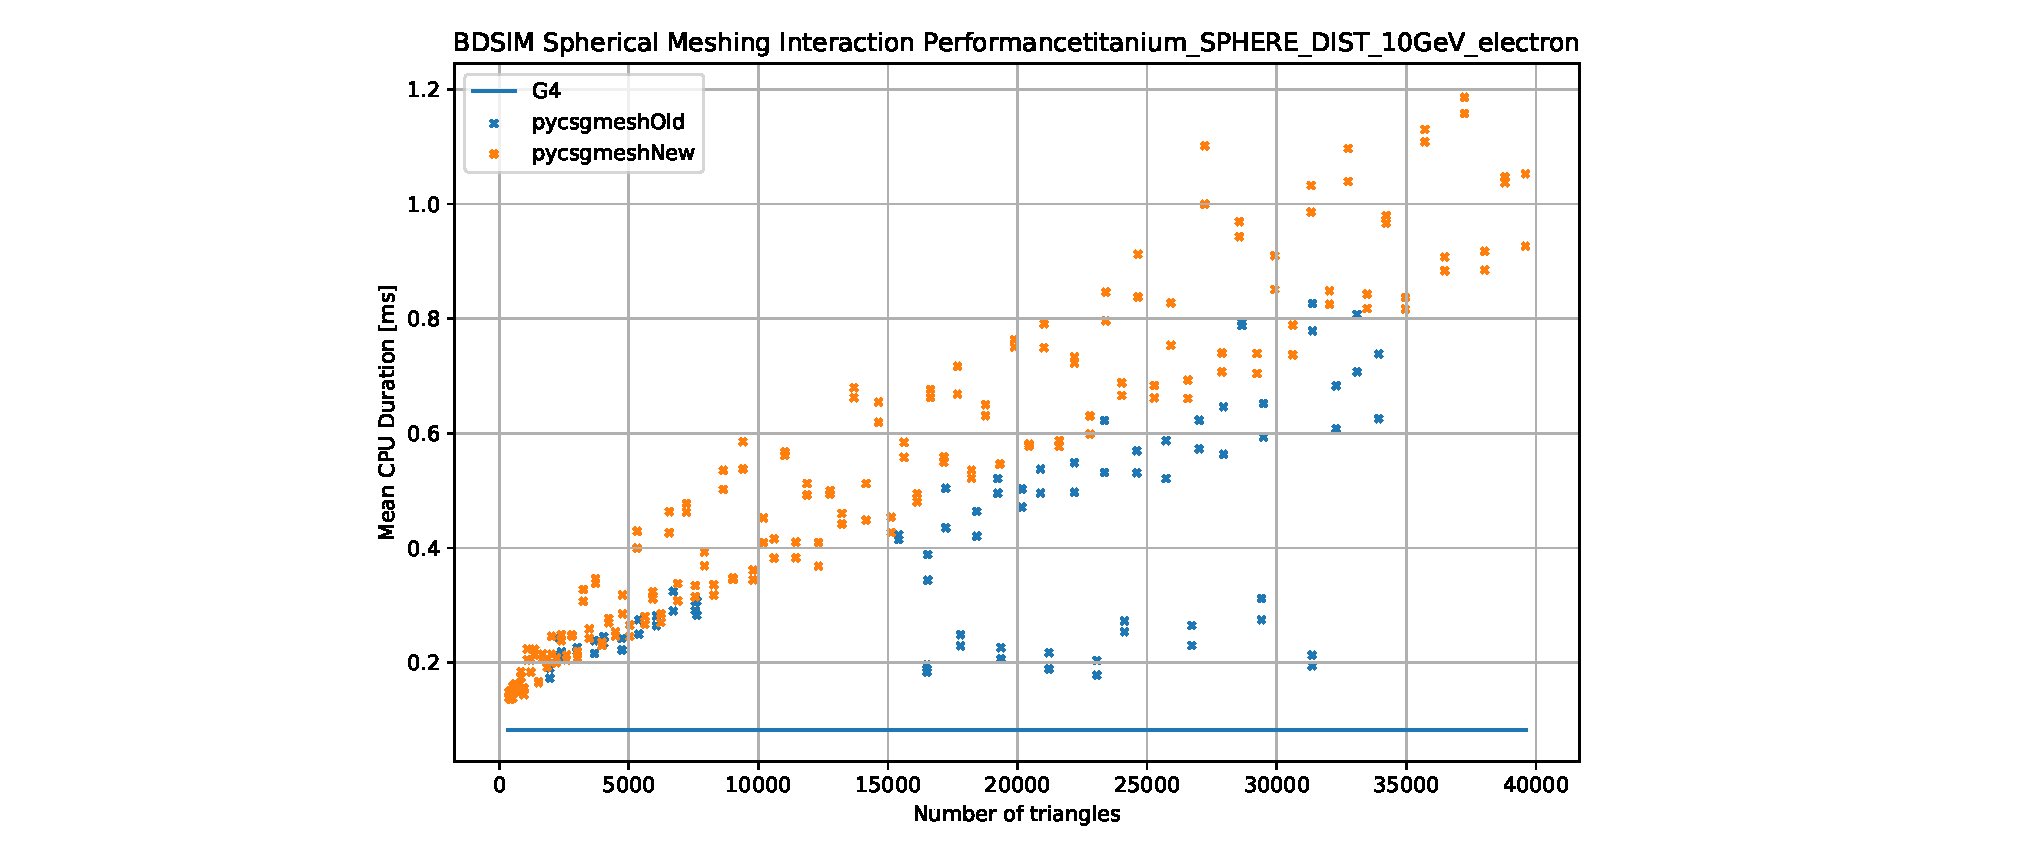
\includegraphics[scale=0.5]{Images//BDSIM//numoftris_tit_10G_e_nostd.pdf}
%\caption[width=\columnwidth]{TODO}
%\label{tubspic}
%\end{figure}

\subsection{Interactions with CAD}
As a final goal to round off the project, an imported CAD model was compared with a compound boolean meshed solid of a generic bolt, shown in Figure \ref{notmybolt}. The CAD bolt was downloaded as a STEP format from a free online database GradCAD \cite{cadmag}. The downloaded model was converted to GDML format with the material G4\_STAINLESS-STEEL using Python. The dimensions of the CAD model were gained by using the measuring tool within the Freecad GUI as shown Figure \ref{boltinfreecad}. The CAD model was then approximately recreated by the constructed of basic primitive solids with boolean operations in Pyg4ometry and can be seen in Figure \ref{boltinvtk}.

\begin{figure}[h!]
\centering
\begin{minipage}{.7\textwidth}
  \centering
  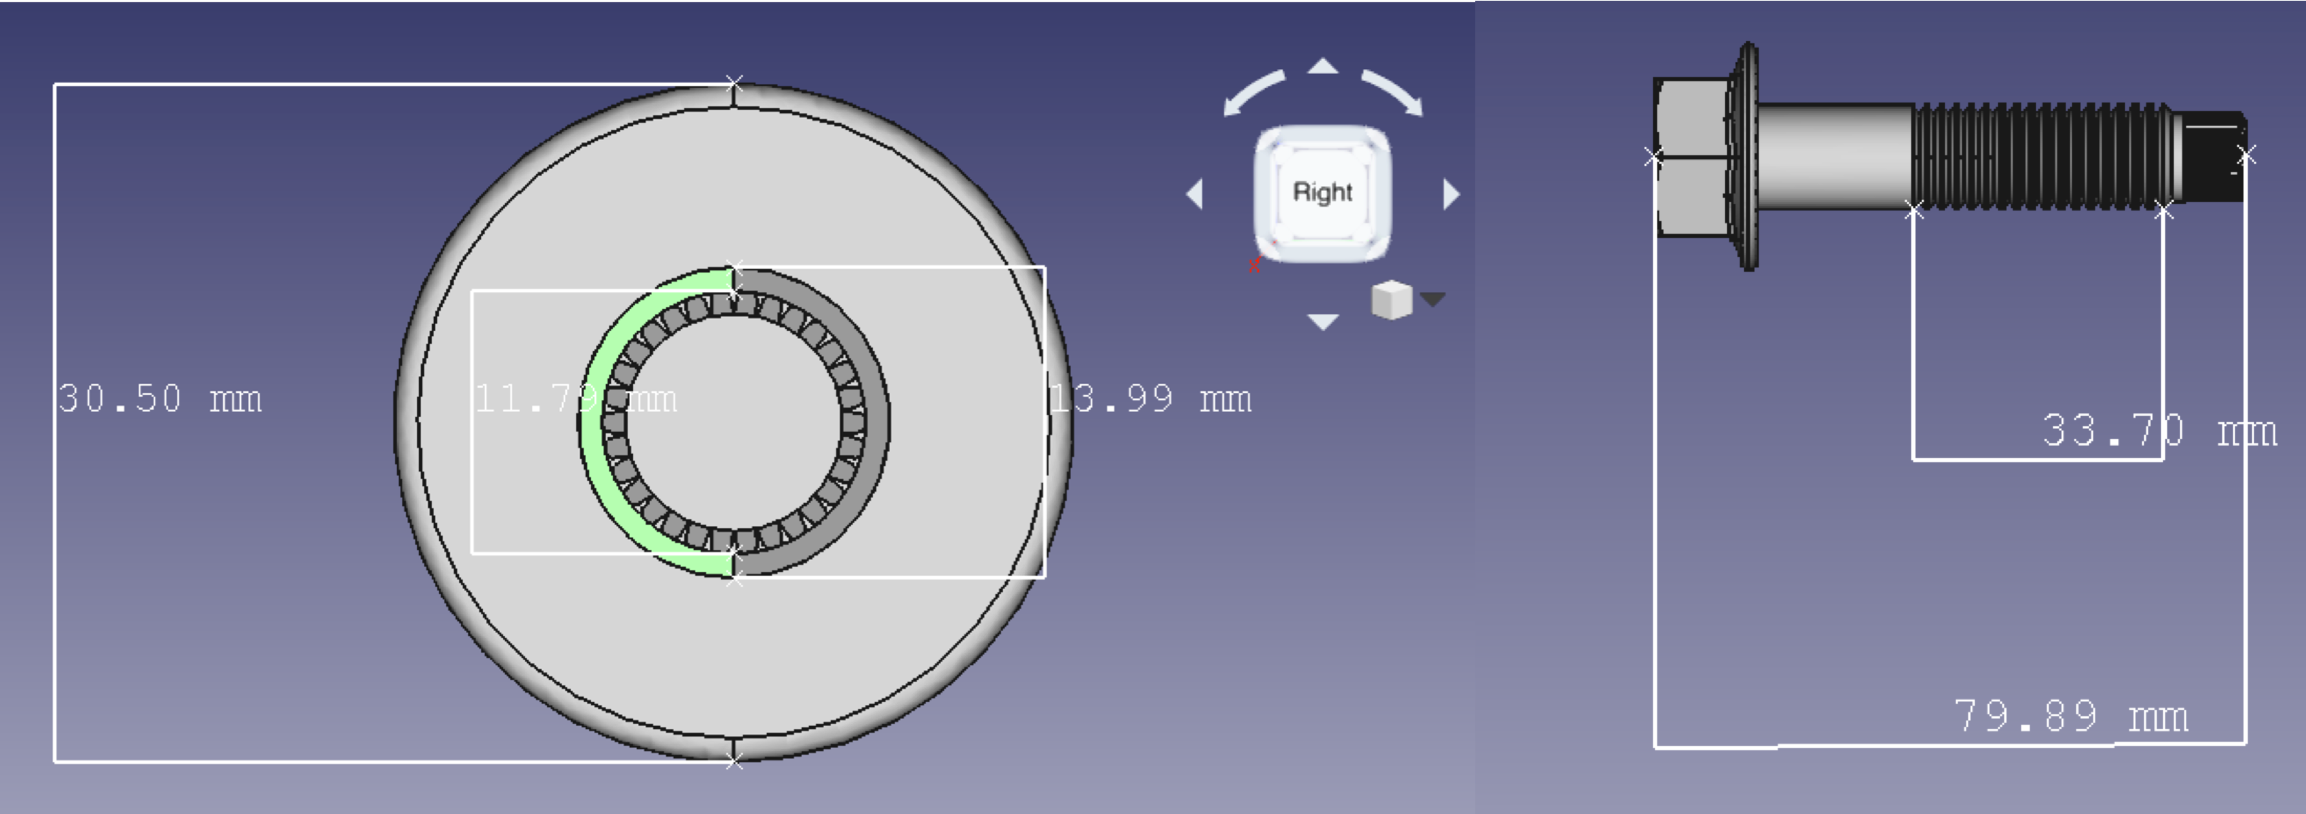
\includegraphics[width=1\textwidth]{Images//CAD_Screw//freecadbolt.png}
  \captionof{figure}{Diagram of imported CAD model in Freecad, with\\ dimensions indicated via Freecad's measuring tool.}
  \label{boltinfreecad}
\end{minipage}%
\begin{minipage}{.3\textwidth}
  \centering
  \vspace{5mm}
  \hspace{2cm}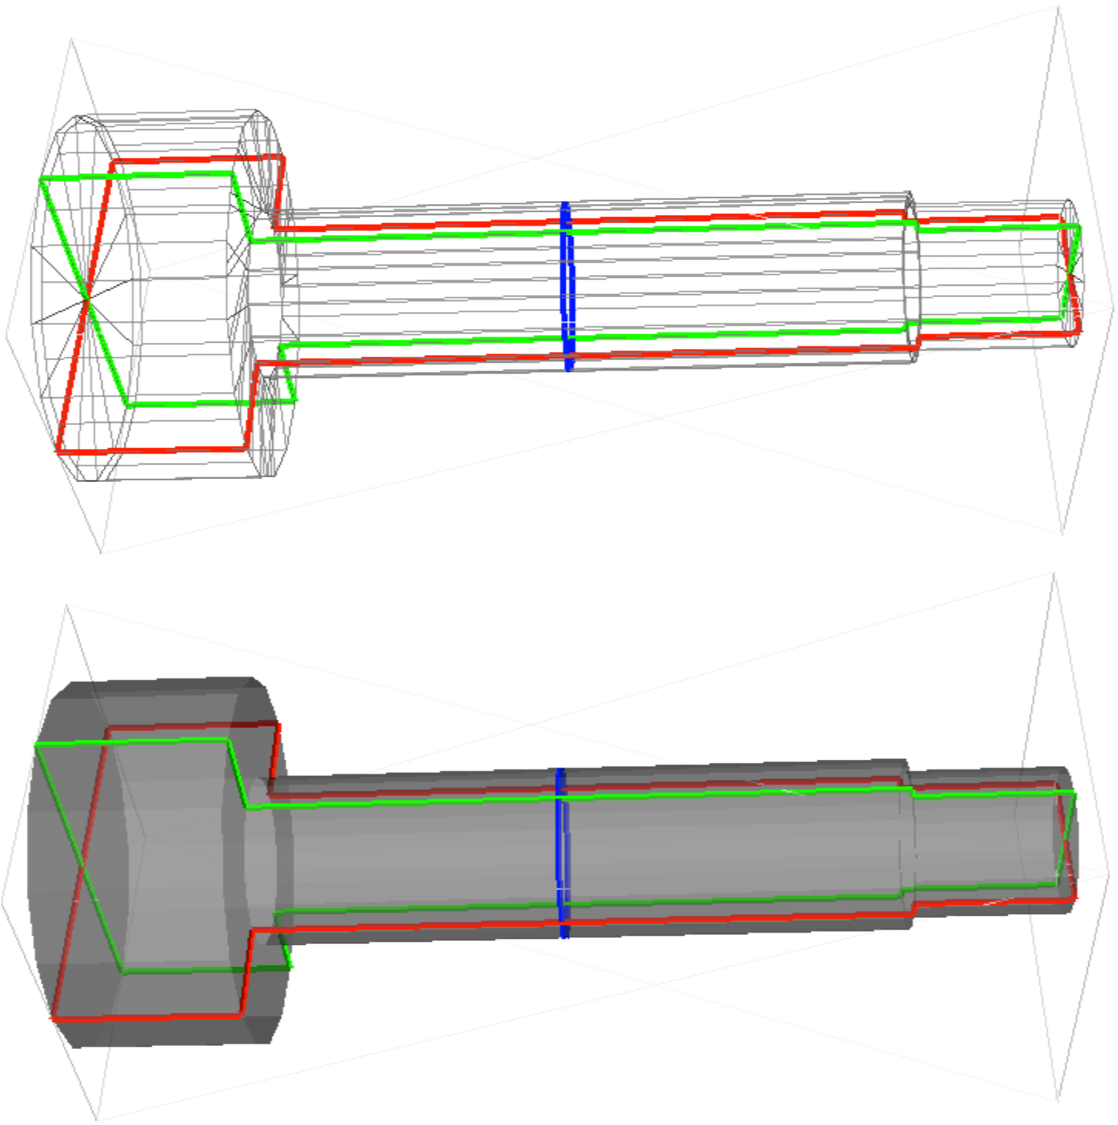
\includegraphics[width=0.9\textwidth]{{Images//CAD_Screw//boltVTK.png}}
  \hspace{5cm}\captionof{figure}{Compund boolean\\ soild recreation of imported\\ CAD model, shown in VTK.}
  \label{boltinvtk}
\end{minipage}%
\end{figure}

\newpage

\begin{figure}[h!]
\centering
\begin{minipage}{.5\textwidth}
  \centering
  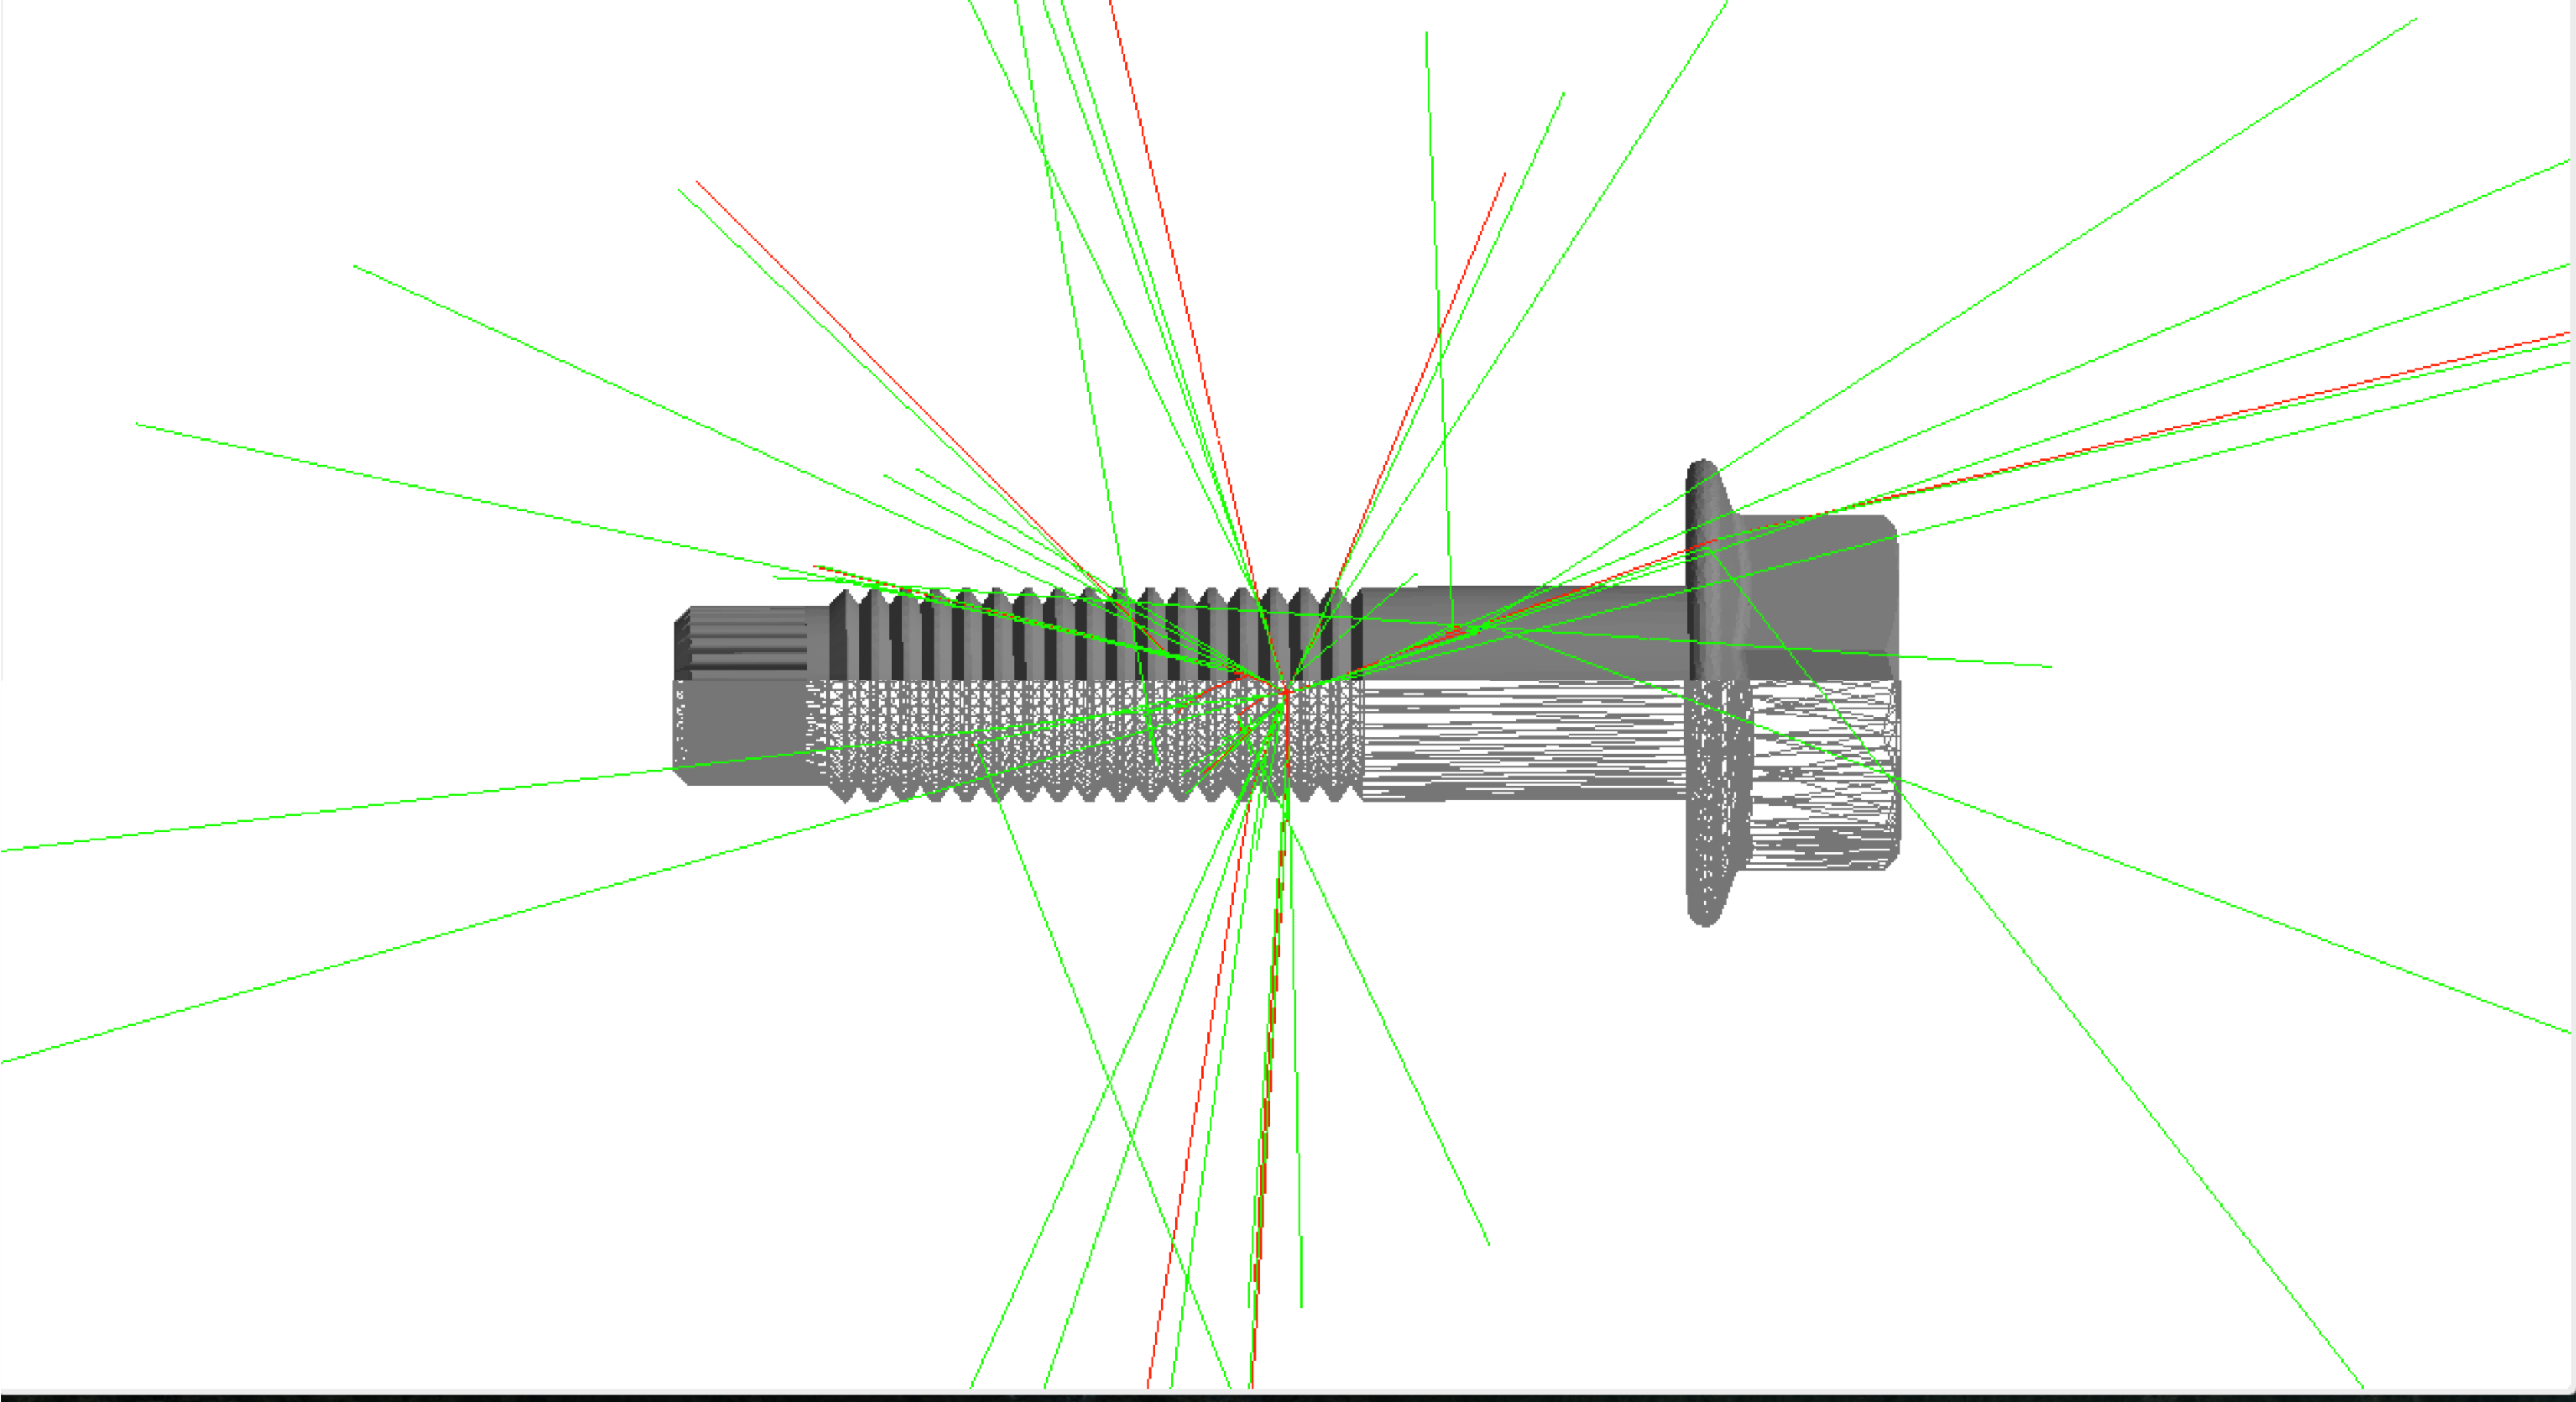
\includegraphics[height=.5\linewidth]{Images//CAD_Screw//Screw_hnh_10MeVe.png}
  \captionof{figure}{A Screenshot of the imported CAD\\ bolt in BDSIM interacting with 10,000 10 MeV\\ electrons}
  \label{notmybolt}
\end{minipage}%
\begin{minipage}{.5\textwidth}
  \centering
  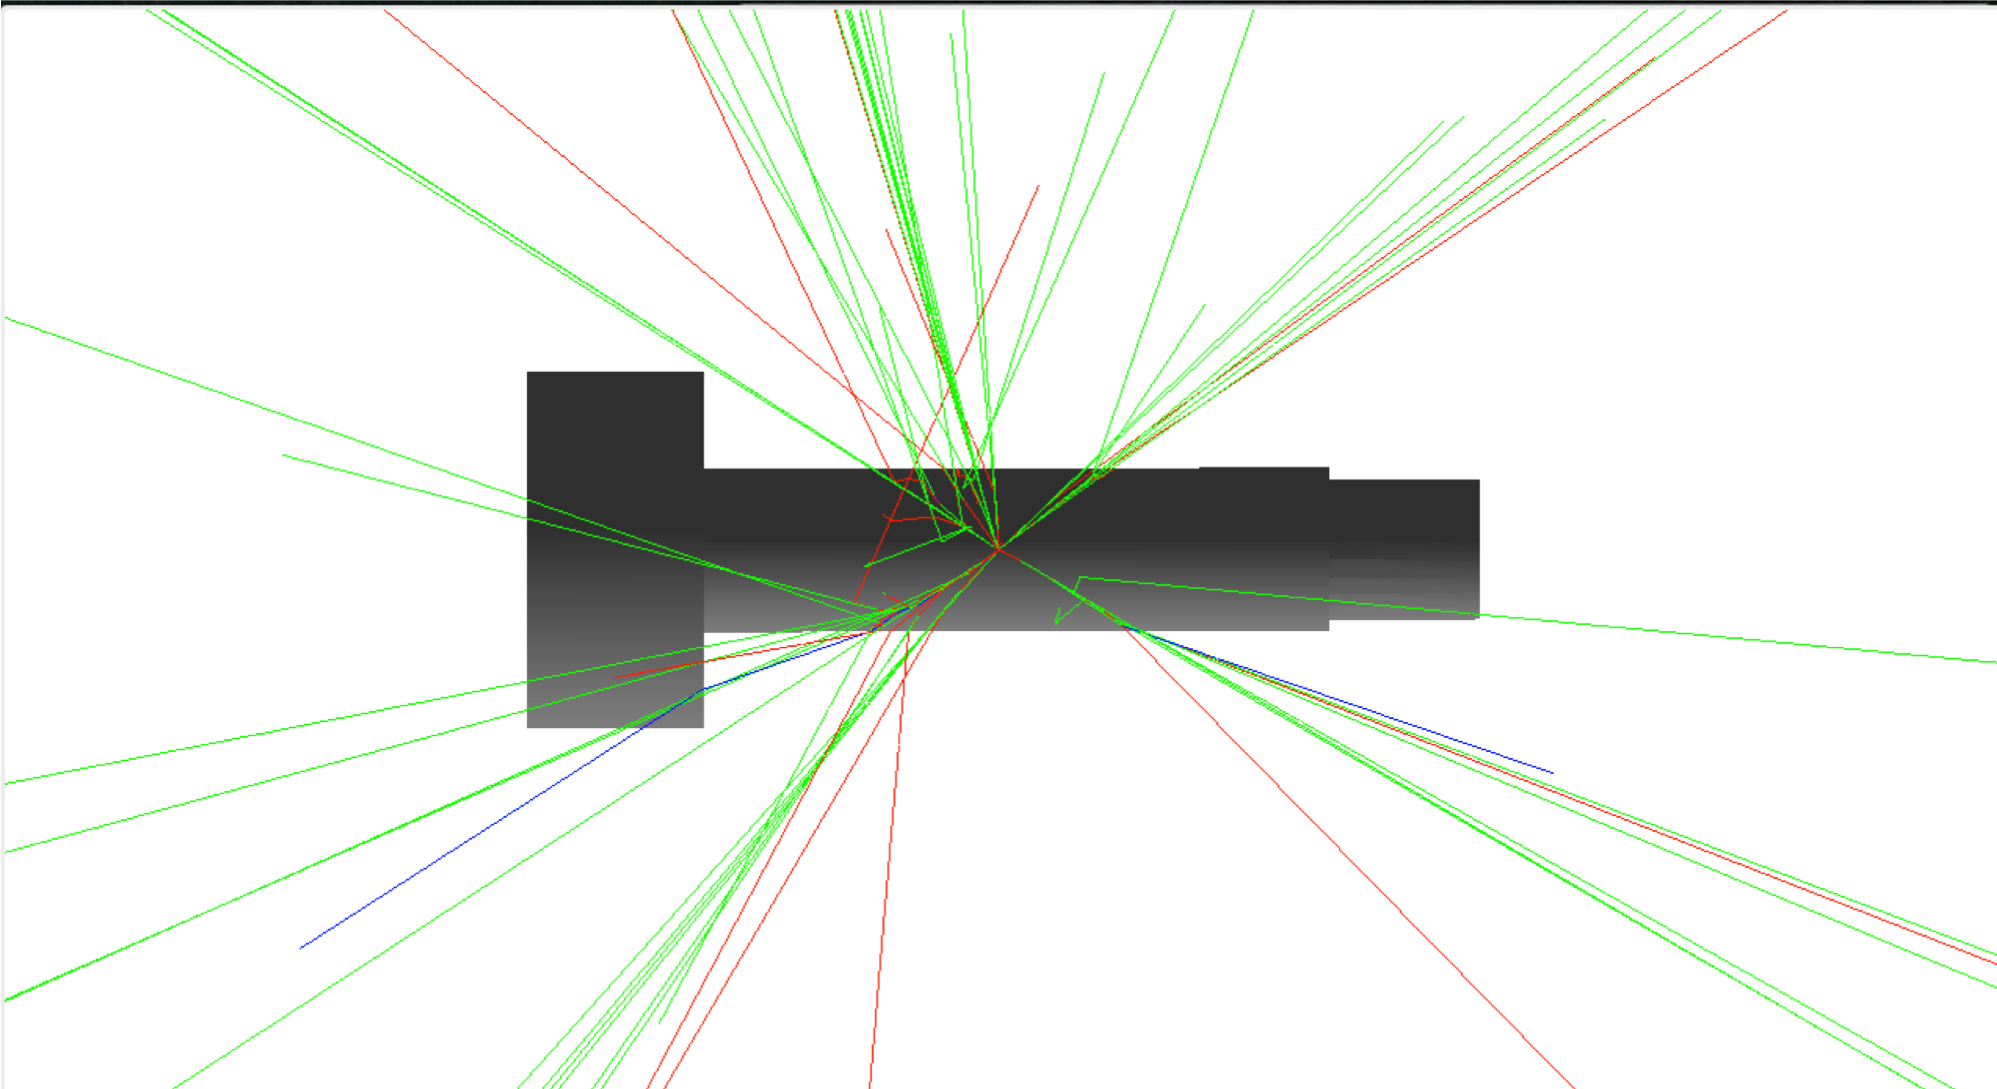
\includegraphics[height=.5\linewidth]{Images//CAD_Screw//bensboltinbdsim.png}
  \captionof{figure}{A Screenshot of the boolean CAD\\ bolt in BDSIM interacting with 10,000 10 MeV\\ electrons}
  \label{mybolt}
\end{minipage}%
\end{figure}

\noindent Both bolts were then ran in BDSIM interacting with a batch of 10,000 electrons through a range of energies 1 MeV to 0.75 TeV. The interactions were simulated using the spherical beam distribution origined at the centre of each bolt, as shown in Figures \ref{notmybolt} \& \ref{mybolt} (same method that was used for spheres in previous Section \ref{}). Figure \ref{boltcount} show the average number of tracks produced from 3 different runs, using a set seed for each run, for both the boolean and CAD bolts. The number of tracks is calculated by subtracting the 10,000 tracks made by the initial electrons from the total number of particle tracks per event extracted using PyBDSIM (Section\ref{pyb}).

\begin{figure}[h!]
\centering
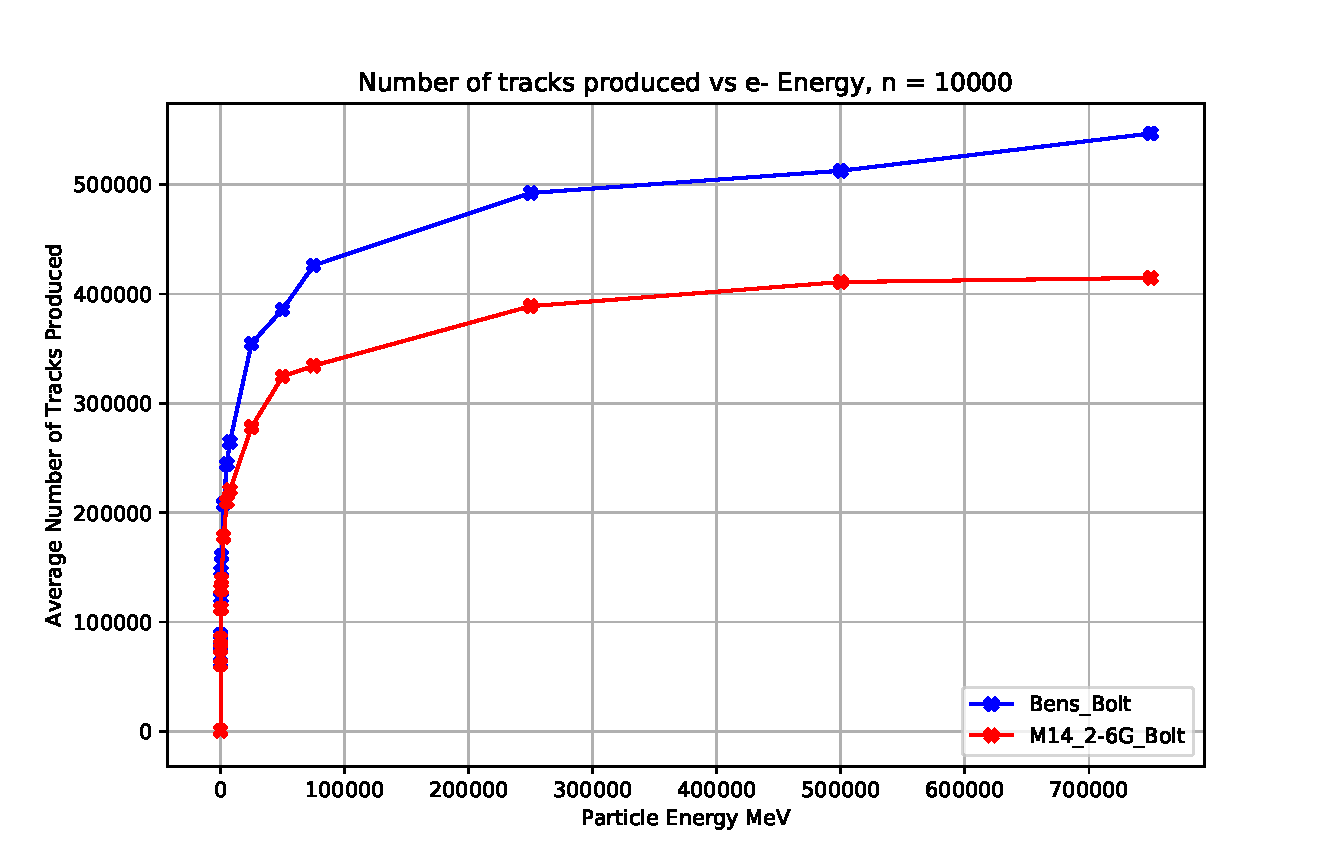
\includegraphics[width=1\textwidth]{Images//CAD_Screw//boltcount.pdf}
\caption[width=\columnwidth]{A plot showing the average number of particle tracks produced in BDSIM when interacting 10,000 electrons of 10 Mev with different targets.}
\label{boltcount}
\end{figure}

\noindent It can be seen that as the energy is increased the electrons generate more secondary particles causing the increase in tracks being stored in BDSIM. The gradient of the data begins to flatten out in the range of 100,000 MeV (100 GeV). This flattening is due to the interactions leading to shower of secondary particles occuring earlier and earlier as the particle energy is increased. Theoretically the graph will then begin to have small drop back down due to ...\\
However due to time constraints and the purpose of the plot being to find the energy range where the number of secondary particles is at large amount for better sampling.
\\\\
\noindent The reason for the number of secondaries being consistently larger for the boolean constructed bolt (Bens\_Bolt) compared with the imported CAD bolt (M14\_2-6G\_Bolt), is most likely due to the boolean construction being an overestimation of the imported bolt. The over estimation would be as a result of  time constraints and ease. The most naive  the threads on the bolt were ignored as well as the the hexagonal and cone features on the head of the bolt.

\begin{figure}[h!]
\centering
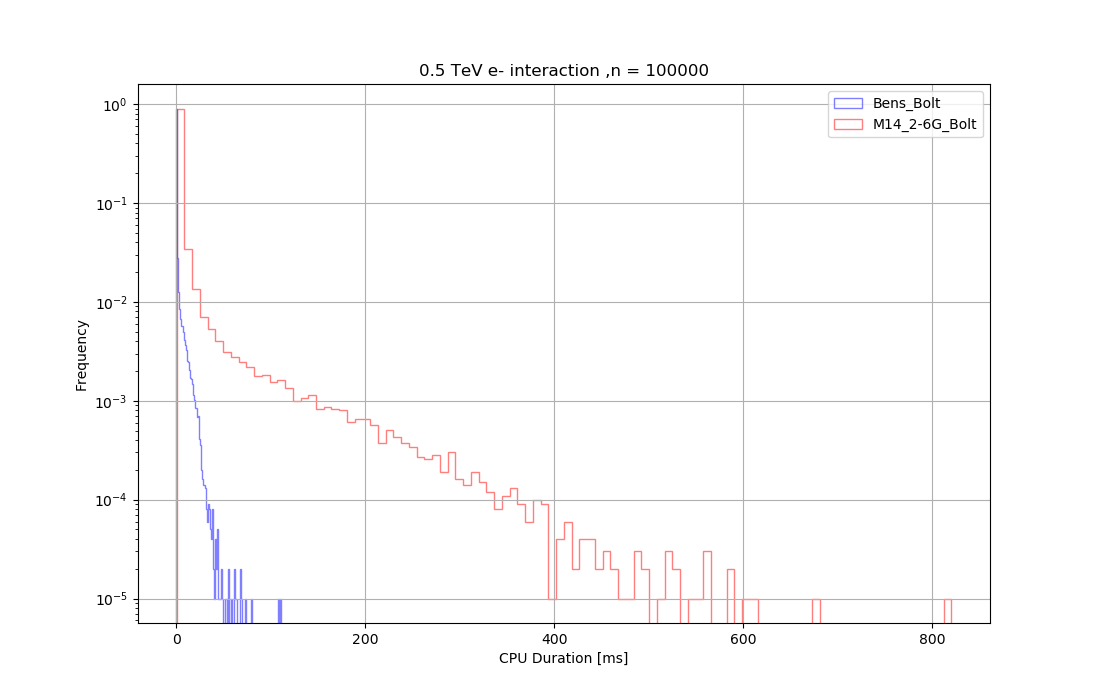
\includegraphics[scale=0.5]{Images//CAD_Screw//cpudist1.png}
\caption[width=\columnwidth]{TODO}
\label{brgqebafd}
\end{figure}


\newpage
\section{Conclusion \& Summary}
\label{conc}

\subsection{Improvements}
meshing is quicker\\
BDSIM interactions are quicker but still slower than G4 solid (as expected)
improved coverage unit test speeds\\
meshing is neater and more uniform in structure\\
higher meshing density = closer to true solid as expected with BDISM interactions\\
quote graphs and sections\\

\subsection{Applications}
As discussed in the introduction (Section \ref{intro} there are many invaluable uses for softwares such as BDSIM and Pyg4ometry that can be used to to aid not only the scientific research community of particle physicist, but also help everyday people by improving medical treatment. Thanks to the software being open source and its wide range of compatible files it can be used to simulate a growing number of projects. This report demonstrates this by CAD magnet modelling.

\subsection{Extension}
If given more time there is several things that I  would have wished to pursue in addition to the project. One being that the analysis done on a sphere in Section \ref{} to also be performed on every one of the remeshed curved primitive solids, all of which are listed in the Appendix \ref{}. This way you could have gain an even more complete picture of the improvement to the meshing of compound solids. Despite a lot of the plots being normalised over a few seed values and being ran with 10,00 of more initial particles, the simulations could be re reran with a more particles and for a larger number of seeds. Also a range of particles other than the electrons such as proton\\
Another area that could have been explored in more detail is a prototype magnet in which I began to make , can be seen in the Appendix \ref{}.

% ------------------------------------------------------------------------------------------------------------------------------
\newpage
\newpage
\footnotesize
\begin{thebibliography}{1}

	\bibitem{vtk}
	vtk homepage\\
	Taken on 10/03/2020\\
	\url{https://vtk.org/}

	\bibitem{spacesh}
	Veli Capali etal.\\
	GEANT4 calculations for space radiation shielding material $Al_2O_3$\\
	DOI: 10.1051/epjconf/201510002002\\

	\bibitem{sat}
	gradcad satellite\\
	Taken on 10/11/2019\\	
	\url{https://grabcad.com/library/gps-satellite-1}

	\bibitem{cern}
	CERN Homepage\\
	Taken on 08/03/2020\\
	\url{https://home.cern/}
	
	\bibitem{magf}
	Geoffrey A. Landis\\
	NASA Lewis Research Center\\
	Magnetic radiation shielding: An idea whose time has returned?\\
	May 15-19, 1991, Princeton, N.J.\\
	Cleveland, OH 44135\\
	U.S.A.
	\url{https://doi.org/10.1063/1.42056}
	
	\bibitem{jai}
	JAI Homepage\\
	Taken on 07/03/2020\\
	\url{https://www.adams-institute.ac.uk/}

	\bibitem{pyg4om}
	Stewart Boogert et al.\\
	Pyg4ometry : A tool to create geometries for GEANT4, BDSIM, G4BEAMLINE and FLUKA for particle loss energy deposition studies\\
	\url{http://accelconf.web.cern.ch/AccelConf/ipac2019/papers/wepts054.pdf}

	\bibitem{bitb}
	Pyg4ometry BitBucket\\
	Taken on 01/03/2020\\
	\url{https://bitbucket.org/jairhul/Pyg4ometry/src/}
	
	\bibitem{}
		BDSIM Manual\\
		Taken on 01/03/2020\\
		\url{http://www.pp.rhul.ac.uk/bdsim/manual/}
		
	\bibitem{bdsimpap}
		L.J Nevay et al.\\
		BDSIM: An accelerator tracking code with particle–matter interactions\\
		\url{https://doi.org/10.1016/j.cpc.2020.107200}
		
	\bibitem{st}
		Sourcetree\\
		Taken on 01/03/2020\\
		\url{https://www.sourcetreeapp.com/}
		
	\bibitem{g4beam}
	\url{https://accelconf.web.cern.ch/accelconf/PAC2011/papers/mop152.pdf}
		
	\bibitem{solids}
	GEANT4 Solids\\
	Taken on 01/03/2020\\
	\url{http://GEANT4-userdoc.web.cern.ch/GEANT4-userdoc/UsersGuides/ForApplicationDeveloper/html/Detector/Geometry/geomSolids.html}
	
	\bibitem{mater}
	GEANT4 Materials\\
	Taken on 01/03/2020\\
	\url{http://GEANT4-userdoc.web.cern.ch/GEANT4-userdoc/UsersGuides/ForApplicationDeveloper/html/Appendix/materialNames.html}
	
	\bibitem{meh}
	M. Pinto, P. Gon\c{c}alves\\
	GUIMesh: A tool to import STEP geometries into GEANT4 via GDML\\
	\url{https://doi.org/10.1016/j.cpc.2019.01.024}
		
	\bibitem{pdg}
	M. Tanabashi et al\\
	43. Monte Carlo Particle Numbering Scheme\\
	\url{http://pdg.lbl.gov/2019/reviews/rpp2019-rev-monte-carlo-numbering.pdf}
	
	\bibitem{stpdat}
	U.S. department of Commerce\\
	Stopping Powers and Ranges of
	Electrons and Positrons\\
	\url{https://www.govinfo.gov/content/pkg/GOVPUB-C13-139be796c7e56cb34375ad52db8ec5e7/pdf/GOVPUB-C13-139be796c7e56cb34375ad52db8ec5e7.pdf}
	
\bibitem{cadmag}
	GrabCad\\
	Source of CAD M14 2-6G Bolt\\
	Taken on 07/03/2020\\
	\url{https://grabcad.com/library/m14-2-1}

\bibitem{cancer}
	Elaine M.Zeman et al.\\
	Abeloff's Clinical Oncology (Sixth Edition)\\
	27 - Basics of Radiation Therapy\\
	\url{https://www.sciencedirect.com/science/article/pii/B978032347674400027X}
	
\bibitem{stprg}
	Machaka, Ronald\\
	Ion Beam Modifications of Boron Nitride By Ion Implantation\\
	2007\\
	\url{https://www.researchgate.net/publication/265496484_Ion_Beam_Modifications_of_Boron_Nitride_By_Ion_Implantation}
	
\bibitem{emo}
	Geant Em0\\
	\url{http://GEANT4-data.web.cern.ch/GEANT4-data/releases/GEANT4/examples/extended/electromagnetic/TestEm0/README}

\bibitem{dose}
	Tsukasa Aso et al.\\
	Optimization of Patient Geometry Based on CT Data in GEANT4 for Medical Application\\
	\url{https://doi.org/10.1016/j.meddos.2017.08.007}

\bibitem{blue}
	Yi Hu et al.\\
	Cherenkov Radiation Control via Self-accelerating Wave-packets\\
	\url{https://www.nature.com/articles/s41598-017-08705-4.pdf}

\bibitem{18}
	freecad 0.18 release notes\\
	\url{https://wiki.freecadweb.org/Release_notes_0.18}

\end{thebibliography}

% ------------------------------------------------------------------------------------------------------------------------------
\normalsize
\newpage
\appendix
\section{Appendix (Python scripts)}
\subsection{Sphere BDSIM Vary Mesh Test}
\label{ap1}
\lstinputlisting[language=Python]{Scripts//Run_New_Meshes.py}

%\newpage
%\subsection{Discovery method contribution pie chart (Figure \ref{pie})}\label{ap2}
%\lstinputlisting[language=Python]{Python//pi.py}

\newpage
\small
\twocolumn[\section{All Meshed Solids and Polygon Count Plots}
\label{app1}
The following Figures are the meshing and polygon data for each primitive solid constructed in Pyg4ometry \ref{pyg}. The first Figure for each solid is a screenshot of the old meshing and new meshing visualized in VTK. They show the before and after of each primitive solid in both solid and meshed view. The second Figures Show the number of polygons and triangles produced on a solid as you increase the slice across a range of 10-100 (if there is a stack it is kept at a constant 10). All plots are made using Python and the sold naming convention is the one used by GEANT4 \ref{g4}\\.]
\begingroup
\subsubsection{Cons}
\begin{figure}[h!]
\centering
\begin{minipage}{.2\textwidth}
  \centering
  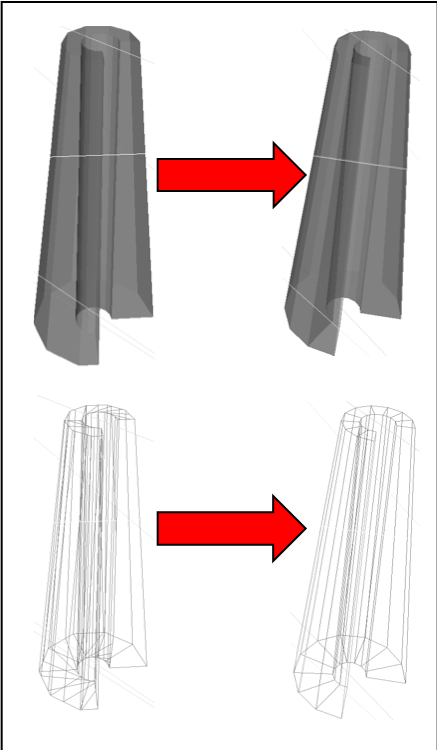
\includegraphics[height=1\linewidth]{Images//Meshes//cons.png}
  \captionof{figure}{}
  \label{cons}
\end{minipage}%
\begin{minipage}{.3\textwidth}
  \centering
  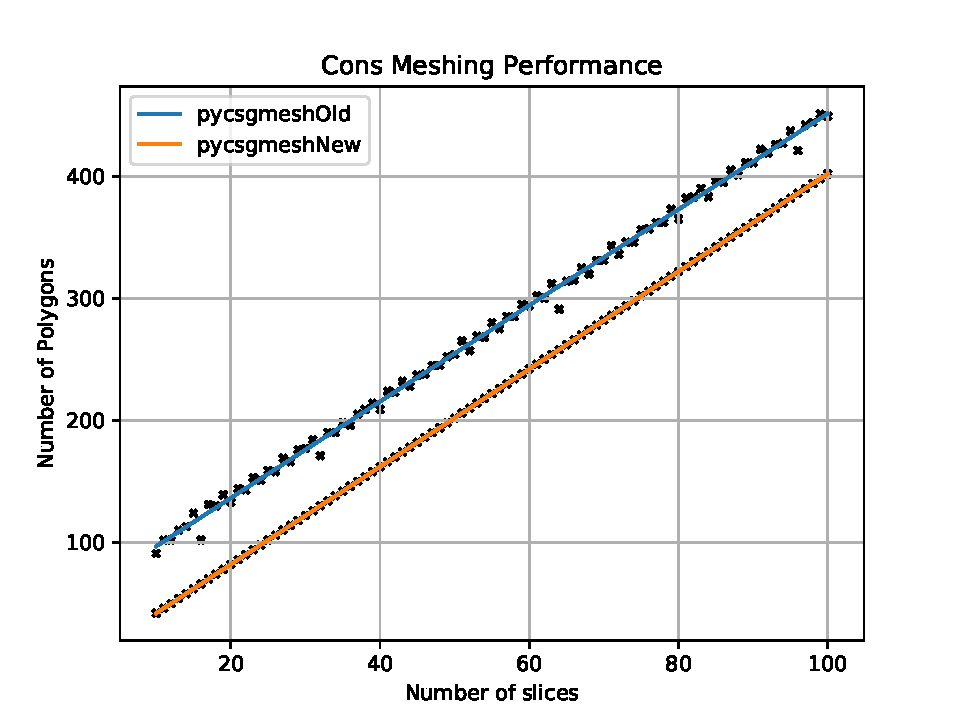
\includegraphics[scale=0.35]{Images//Quad_fits//Cons_quad.pdf}
  \captionof{figure}{ }
  \label{fig:test2}
\end{minipage}%
\end{figure}

\subsubsection{CutTubs}

\begin{figure}[h!]
\centering
\begin{minipage}{.2\textwidth}
  \centering
  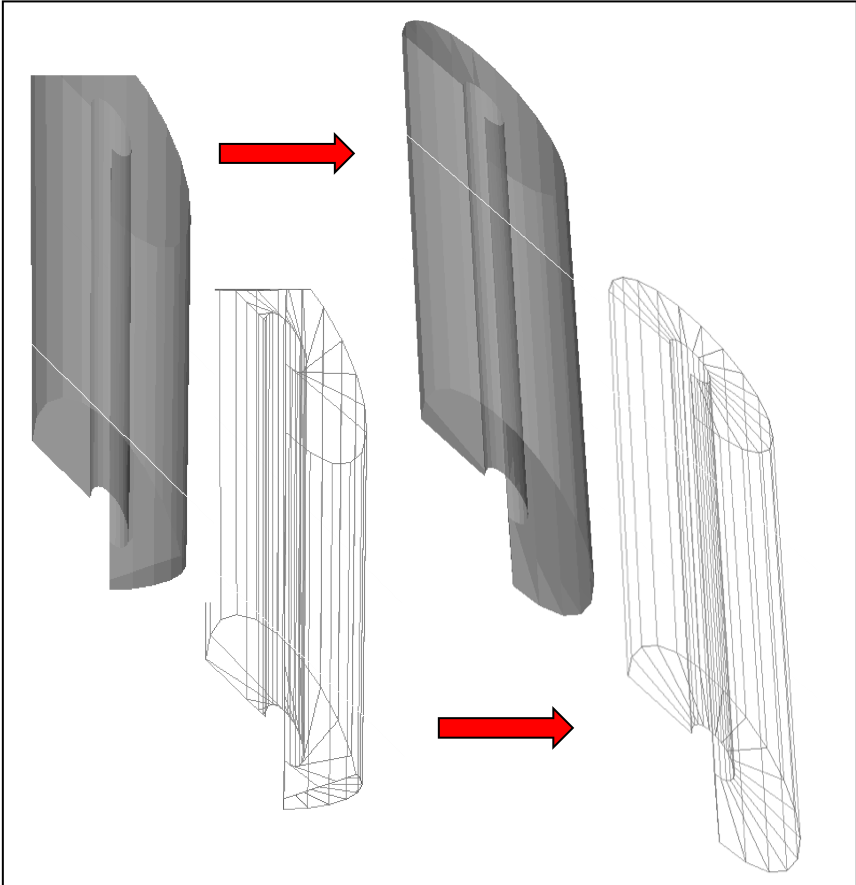
\includegraphics[height=1\linewidth]{Images//Meshes//CutTubs.png}
  \captionof{figure}{ }
  \label{ctub}
\end{minipage}%
\begin{minipage}{.3\textwidth}
  \centering
  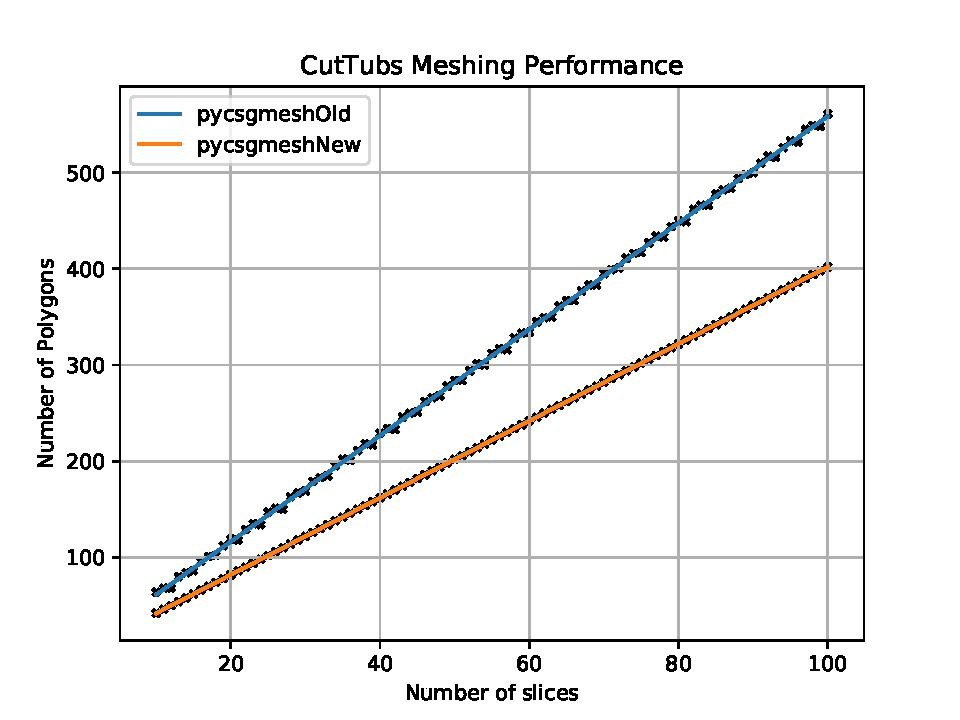
\includegraphics[scale=0.35]{Images//Quad_fits//CutTubs_quad.pdf}
  \captionof{figure}{ }
  \label{}
\end{minipage}%
\end{figure}
\subsubsection{Ellipsoid}

\begin{figure}[h!]
\centering
\begin{minipage}{.2\textwidth}
  \centering
  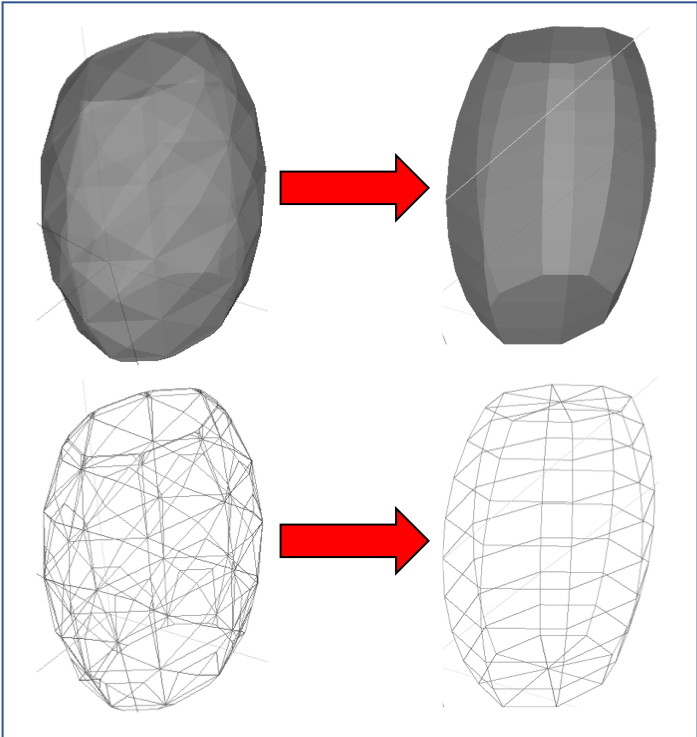
\includegraphics[height=1\linewidth]{Images//Meshes//ellipsoid.png}
  \captionof{figure}{ }
  \label{fig:test1}
\end{minipage}%
\begin{minipage}{.3\textwidth}
  \centering
  \includegraphics[scale=0.35]{Images//Quad_fits//Ellipsoid_quad.pdf}
  \captionof{figure}{ }
  \label{fig:test2}
\end{minipage}%
\end{figure}

\newpage
\subsubsection{EllipticalCone}

\begin{figure}[h!]
\centering
\begin{minipage}{.2\textwidth}
  \centering
  \includegraphics[height=1\linewidth]{Images//Meshes//ellipticalcone.png}
  \captionof{figure}{ }
  \label{fig:test1}
\end{minipage}%
\begin{minipage}{.3\textwidth}
  \centering
  \includegraphics[scale=0.35]{Images//Quad_fits//Ellipticalcone_quad.pdf}
  \captionof{figure}{ }
  \label{fig:test2}
\end{minipage}%
\end{figure}

\subsubsection{EllipticalTube}

\begin{figure}[h!]
\centering
\begin{minipage}{.2\textwidth}
  \centering
  \includegraphics[height=0.8\linewidth]{Images//Meshes//ellipticaltube.png}
  \captionof{figure}{ }
  \label{fig:test1}
\end{minipage}%
\begin{minipage}{.3\textwidth}
  \centering
  \includegraphics[scale=0.35]{Images//Quad_fits//EllipticalTube_quad.pdf}
  \captionof{figure}{ }
  \label{fig:test2}
\end{minipage}%
\end{figure}

\subsubsection{Hyperboloid}

\begin{figure}[h!]
\centering
\begin{minipage}{.2\textwidth}
  \centering
  \includegraphics[height=0.9\linewidth]{Images//Meshes//hyperboloid.png}
  \captionof{figure}{ }
  \label{fig:test1}
\end{minipage}%
\begin{minipage}{.3\textwidth}
  \centering
  \includegraphics[scale=0.35]{Images//Quad_fits//Hyperboloid_quad.pdf}
  \captionof{figure}{ }
  \label{fig:test2}
\end{minipage}%
\end{figure}

\newpage
\subsubsection{Orb}

\begin{figure}[h!]
\centering
\begin{minipage}{.2\textwidth}
  \centering
  \includegraphics[height=0.8\linewidth]{Images//Meshes//orb.png}
  \captionof{figure}{ }
  \label{Sphere}
\end{minipage}%
\begin{minipage}{.3\textwidth}
  \centering
  \includegraphics[scale=0.35]{Images//Quad_fits//orb_quad.pdf}
  \captionof{figure}{ }
  \label{fig:test2}
\end{minipage}%
\end{figure}

\subsubsection{Paraboloid}

\begin{figure}[h!]
\centering
\begin{minipage}{.2\textwidth}
  \centering
  \includegraphics[height=1\linewidth]{Images//Meshes//paraboloid.png}
  \captionof{figure}{ }
  \label{para}
\end{minipage}%
\begin{minipage}{.3\textwidth}
  \centering
  \includegraphics[scale=0.35]{Images//Quad_fits//Paraboloid_quad.pdf}
  \captionof{figure}{ }
  \label{fig:test2}
\end{minipage}%
\end{figure}

\subsubsection{Polycone}
\begin{figure}[h!]
\centering
\begin{minipage}{.2\textwidth}
  \centering
  \includegraphics[height=1\linewidth]{Images//Meshes//polycone.png}
  \captionof{figure}{ }
  \label{fig:test1}
\end{minipage}%
\begin{minipage}{.3\textwidth}
  \centering
  \includegraphics[scale=0.35]{Images//Quad_fits//Polycone_quad.pdf}
  \captionof{figure}{ }
  \label{fig:test2}
\end{minipage}%
\end{figure}

\newpage
\subsubsection{Sphere}

\begin{figure}[h!]
\centering
\begin{minipage}{.2\textwidth}
  \centering
  \includegraphics[height=0.75\linewidth]{Images//Meshes//sphere.png}
  \captionof{figure}{ }
  \label{fig:test1}
\end{minipage}%
\begin{minipage}{.3\textwidth}
  \centering
  \includegraphics[scale=0.35]{Images//Quad_fits//Sphere_quad.pdf}
  \captionof{figure}{ }
  \label{fig:test2}
\end{minipage}%
\end{figure}

\subsubsection{Torus}

\begin{figure}[h!]
\centering
\begin{minipage}{.2\textwidth}
  \centering
  \includegraphics[height=0.5\linewidth]{Images//Meshes//torus.png}
  \captionof{figure}{ }
  \label{fig:test1}
\end{minipage}%
\begin{minipage}{.3\textwidth}
  \centering
  \includegraphics[scale=0.35]{Images//Quad_fits//Torus_quad.pdf}
  \captionof{figure}{ }
  \label{fig:test2}
\end{minipage}%
\end{figure}

\subsubsection{Tubs}

\begin{figure}[h!]
\centering
\begin{minipage}{.2\textwidth}
  \centering
  \includegraphics[height=0.7\linewidth]{Images//Meshes//tubs.png}
  \captionof{figure}{ }
  \label{fig:test1}
\end{minipage}%
\begin{minipage}{.3\textwidth}
  \centering
  \includegraphics[scale=0.35]{Images//Quad_fits//Tubs_quad.pdf}
  \captionof{figure}{ }
  \label{fig:test2}
\end{minipage}%
\end{figure}

\endgroup
\onecolumn
\section{Quadratic Parameters for polygon count plots}
\label{appp1}
The quadratic fit where its parameters are of the form:
\begin{equation}
ax^2 + bx + c = 0
\end{equation}

\small
% Table generated by Excel2LaTeX from sheet 'Sheet1'
\begin{table}[htbp]
  \small
  \centering
  \caption{A Table showing the parameters to the quadratic fits for the polygon count plot.}
    \begin{tabular}{lrrrrrr}
    Curved Primitive Solid & \multicolumn{1}{l}{Old a} & \multicolumn{1}{l}{Old b} & \multicolumn{1}{l}{Old c} & \multicolumn{1}{l}{New a} & \multicolumn{1}{l}{New b} & \multicolumn{1}{l}{New c} \\
    Cons  & -2.74E-04 & 3.97E+00 & 5.72E+01 & -3.83E-17 & 4.00E+00 & 2.00E+00 \\
    CutTubs & 2.19E-04 & 5.50E+00 & 6.30E+00 & -3.83E-17 & 4.00E+00 & 2.00E+00 \\
    Ellipsoid & 18.65090372 & -333.5688153 & 1919.792901 & 1.61E-17 & 1.20E+01 & 0.00E+00 \\
    EllipticalCone & 4.00E+00 & 2.00E+00 & 2.41E-12 & 4.03E-18 & 3.00E+00 & 0.00E+00 \\
    EllipticalTube & -1.94E-16 & 4.20E+01 & -5.72E-13 & 4.03E-18 & 3.00E+00 & 0.00E+00 \\
    Hyperboloid & 64.83177713 & -1452.629624 & 16378.18198 & 4.84E-17 & 2.20E+01 & -9.53E-14 \\
    Orb   & -6.45E-17 & 3.40E+01 & -1.91E-13 & -8.06E-18 & 1.00E+01 & -4.77E-14 \\
    Paraboloid & -1.94E-16 & 3.40E+01 & -1.91E-13 & 1.61E-17 & 1.20E+01 & 0.00E+00 \\
    Polycone & 0.39682347 & 7.13011557 & 7.42466252 & -4.03E-17 & 6.00E+00 & 4.00E+00 \\
    Sphere & 10.82154926 & -356.6329124 & 8557.249195 & 2.00E+01 & 2.20E+02 & 1.98E-11 \\
    Torus & 7.01776508 & 304.8746037 & 4899.196225 & -1.61E-17 & 2.00E+01 & -9.53E-14 \\
    Tubs  & 0.27241769 & 4.58191175 & 8.33675211 & -3.83E-17 & 4.00E+00 & 2.00E+00 \\
    \end{tabular}%
  \label{tab1}%
\end{table}

\section{Prototype Freecad Magnet}
\label{mag}
First attempt at a prototype magnet made using Freecad GUI (Figure \ref{freee}) and exported as a STEP file, which was then converted to a GDML format with GEANT4 material G4\_Cu using python. A magnet field was then mapped on to the shape using a preset dipole field in BDSIM, in which you can see electrons repelling in Figure \ref{repel}.

\begin{figure}[h!]
\centering
\begin{minipage}{.5\textwidth}
  \centering
  \includegraphics[height=0.5\linewidth]{Images//CAD_Mag//maginfreecad.png}
  \captionof{figure}{Freecad screenshot}
  \label{freee}
\end{minipage}%
\begin{minipage}{.5\textwidth}
  \centering
  \includegraphics[height=.5\linewidth]{Images//CAD_Mag//maginbdsim.png}
  \captionof{figure}{BDSIM screenshot}
  \label{repel}
\end{minipage}%
\end{figure}


\end{document}